\documentclass[letterpaper,twocolumn,openany]{dndbook}

% Use babel or polyglossia to automatically redefine macros for terms
% Armor Class, Level, etc...
% Default output is in English; captions are located in lib/dndstring-captions.sty.
% If no captions exist for a language, English will be used.
%1. To load a language with babel:
%	\usepackage[<lang>]{babel}
%2. To load a language with polyglossia:
%	\usepackage{polyglossia}
%	\setdefaultlanguage{<lang>}
\usepackage[english]{babel}
%\usepackage[italian]{babel}
% For further options (multilanguage documents, hypenations, language environments...)
% please refer to babel/polyglossia's documentation.

\usepackage[utf8]{inputenc}
\usepackage[singlelinecheck=false]{caption}
\usepackage{lipsum}
\usepackage{listings}
\usepackage{shortvrb}
\usepackage{stfloats}

\captionsetup[table]{labelformat=empty,font={sf,sc,bf,},skip=0pt}

\MakeShortVerb{|}

\lstset{%
  basicstyle=\ttfamily,
  language=[LaTeX]{TeX},
  breaklines=true,
}

\title{Velterra{} \\
\large Sinners Never Sleep}
\author{A Dungeons and Dragons Adventure}
\date{2019/07/18}

\begin{document}

\twocolumn

\frontmatter

\maketitle

\onecolumn
\clearpage

\begin{center}
 
\vspace*{10mm} 
 
\Huge
The Cast
\vspace{10mm}

\begin{center}

\includegraphics[width=140mm]{./content/img/teamPhoto.png}
\begin{figure}[h]
\end{figure}
\end{center}



\huge

\textbf{Michael Williams} \\
\textit{Dungeon Master}
\vspace{5mm}

\large

\textbf{Stephen Harland} \\
\textit{Pilcheur Gamont/Mark O'Synne/Vu Dong/Burnie Cinders} \\

\vspace{5mm}

\textbf{Jonathan Mann} \\
\textit{Exmerah Sliokzog}\\

\vspace{5mm}

\textbf{Richard Pugh} \\
\textit{Riphard Obsidian Hardstone}\\

\vspace{5mm}

\textbf{Stephen Reddish} \\
\textit{Kolo Kozolski Sliokzog/Toni The Tiger/Martin AndleBerger}\\

\vspace{5mm}

\textbf{Joshua Rodell} \\
\textit{Lady Otoria Hearthrust/Gary/Myron}  \\

\vspace{5mm}

\end{center}

\clearpage

\tableofcontents

\mainmatter%

\chapter{Characters}
\subsection{Kolo "Toure" Kozolski}
\begin{center}

\includegraphics[width=80mm]{./content/img/krokokolo.png}
\begin{figure}[h]
\end{figure}
\end{center}

\textbf{Details}\\
Race: Goblin\\
Class: Rogue/Ranger\\
Age: 8\\
Status: Dead\bigskip

\textbf{Background}\\
From "the north", Kolo appears to have an existing relationship with the other goblin, Exmerah. Uses a bow and possibly high explosives.\bigskip

\textbf{Personality and Traits}\\
Boisterous and outspoken, Kolo appears to be the face and frontman of the goblin duo.\smallskip
Known for his fast fingers, Kolo is not to be trusted with, or near, anyone's money or property.\smallskip
Speaks Tikki Tuck, Goblin, and Low Velterran\smallskip

\textbf{Relationships}
Twinned with Exmerah.\\
Seems to dislike racist Pilch, refering to him as "Pilchard" or "fishy fishy" or at least did before Fishy went away.\smallskip
Strangled to death by Riphard with a Cool Whip.

\clearpage
\subsection{Martin Andleberger}
\begin{center}
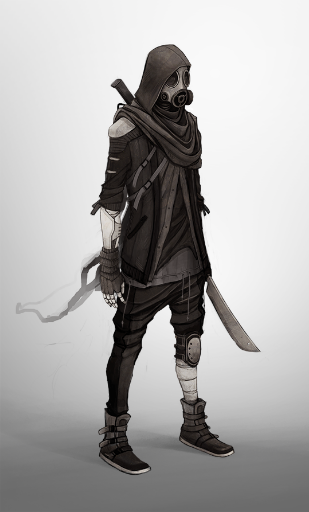
\includegraphics[width=80mm]{./content/img/martin.png}
\begin{figure}[h]
\end{figure}
\end{center}

\textbf{Details}\\
Race: Construct\\
Class: Bard/Sorcerer\\
Age: 87\\
Status: Possibly a Mouse\bigskip

\textbf{Background}\\
The AndelBergers seemed like any other old aristocratic family from Lindedorf, at least from the outside. Who was to know that the family line stretched almost a 1000 years back in history. So far back that the families histories pre-dated the sundering itself.    \medskip

Lord and Lady AndelBergers had been (in)breeding their family ever since the sundering to maintain a pure bloodline, the latest incarnation had proved very difficult indeed as the Lady had only managed to produce a single child, a solitary lady who glowed with the radiance of Hemotate. She was schooled from the families great library and a sense of destiny passed into her. Until one dark and stormy night the church arrived, or at least a part of the church that people only talked about in whispers. Dark masked figures stormed the house and decimated what was left of the family, what happened to the young Ms AndelBerger is still unknown.   \medskip

MarTin was the family butler, built to protect and serve Ms AndelBerger and keep her entertained. He had been fashioned using the knowledge of the ancient family line, his clothes and parts shaped in strange swirling patterns taken from books long useless. On the fateful night the inquisition appeared, Martin was out milking the cows in the freezing rain. He missed the entire saga, only returning to an empty house torn apart at the seems. He rescued his favourite books, and weighed up his options. He had lost everything, but he still had two purposes, to find the young Ms AndelBerger, and to avenge the family line. As possibly the last member of the family line it was now up to him to return the gods to their rightful place within the pantheon.    \medskip

All this was almost a century ago, MarTin has been wandering ever since    \medskip

Unable to die the butler wandered the streets, then the town, then the city, until finally the continent. Until he was chanced upon by a motley crew in an airship....     

\textbf{Personality and Traits}\\
Martin was very depressed, and lacked the spark of power that helps him deal with the day to day drudgery of being immortal. When he discovered the teams goals were to destroy the church he picked himself up only a little bit. It wasn't until he discovered that his ward Ms Andelberger was gone, and ascended to the heavens, that he doubled down and vowed vengeance
Speaks Tikki Tuck, Goblin, and Low Velterran    

\textbf{Relationships}
Martin is forming relationships within the team, he seems most attached to Burnie.\bigskip

\clearpage
\section{Anthony K Tigerius III}

\begin{center}

\includegraphics[width=80mm]{./content/img/toniTiger.jpg}
\begin{figure}[h]
\end{figure}
\end{center}

\subsection*{Details}

Race: DesertCat\\
Class: Barbarian\\
Age: 42\\
Status: Wandering the Expanse with an assassins contract out on him

\subsubsection{Background}

Anthony has been sent from the Guild of Coin in Hopes Rest to open negotiations with one Riphard Obsidian Hardstone.

\subsubsection{Personality and Traits}

Toni saw the possibility of a better world, he did all he could to help ensure that the lessons learned in the desert could help others around him.

\subsubsection{Relationships}

Toni always wanted to work closely with Riphard, who in his mind was an un-tempered prodigy who would take the world by storm. He had big hopes that the power and wealth that Riphard could wield, could be used for the betterment of all in Velterra.\bigskip

\clearpage

\twocolumn
\chapter{Episodes}
\section{Episode 1: Riphard Begins}

\begin{multicols}{2}

\DndDropCapLine{W}elcome to the world of Velterra, domain of the Seven, who rule over all from afar through the constant vigilance of the Church.\medskip

“In Hope’s Rest, the largest city of the Empire of the Seven, a cloaked man dashes over rooftops, a half-burnt tome tucked under one arm as a group of mercenaries chase him. Abruptly he comes to a dead end, a roof with nowhere to leap to and nowhere to hide. He turns to face his attackers and reaches for his weapons, the book slipping from his grasp as he does so. In a moment of panic he spins to grab for the book, losing his balance and toppling from the roof as the mercenaries swing their blades at his back.”\medskip

“In the north, a pair of goblin twins flee the perils of Valkar Varg’s reign, seeking the freedom and new life the south can bring. They are surrounded by brutal tribesmen and vicious axes on all sides, angered by their desertion. As the two goblins look at each other in desperation and anger they nod, the girl raising a long rifle that quivers with electricity, the boy raising a small hunting bow and quickly loosing several arrows. As their enemies close in the bow-user pulls a vial of some mysterious viscous liquid as his twin sister unclips a thrumming round device from her belt. In moments, a huge explosion rips through the area.”\medskip

“To the south, a dwarf pastor sits hunched over a tome, scribbling notes. He raises his head as he hears the slow creak of his door, aware that he is expecting no visitors. He stands and turns to see a hulking figure behind him, armoured with a long-barelled gun at his side. The dwarf rests a trembling hand on his holster as a man who should not exist stands before him. Terse words are exchanged, accusations and threats. The dwarf grits his teeth and sets his feet, drawing the pistol at his side as his opponent does the same. From outside, the sound of a single shot being fired can be heard.”\medskip

“To the East, a figure wrapped in cloth and strange garments sits quietly in a harbour tavern in Port Averdale, recently arrived on the continent from a long voyage. She sits with an untouched mug of unappealing ale in front of her as three thugs approach the table. They slam down a parchment on the table with a picture and a hefty figure. In a flash she is to her feet, blade drawn and two of the men sliced apart on the ground. She faces the remaining thug who whistles and a stream of men pour into the building from all around. Outnumbered by scores and with a demand the surrender, she chooses the only option she knows. Honour.”\medskip

A group of strangers meet up in a featureless, polished stone room, none fully understanding what has brought them there. An elephantine creature (Meredith) beckons them through a mysteriously appearing door into a plush office where a red skinned man wearing a human face mask welcomes them.\medskip

The man explains that he is called Lazarus and that the group have all recently died. They have been brought together, here, and given a second chance at life in exchange for carrying out a mission to destroy the Church Upon asking for proof Pilch is shown the full, gory reality of their situation through a window into hell Lazarus explains that the group must obtain the Stone of Anthala from the temple of XXX and our given basic directions. This ancient relic will be the source of future communications with Lazarus and his means of issuing further instructions. They are warned not to gain the attention of the Church.\medskip

The group agree to carry out the task and are transported into a cavern, where winter clothes and supplies await them. After some brief introductions Exme opens the cave door to reveal they are in a snowy wilderness The group spend two days walking South (Kolo relieves Pilch of 15 gp during the trip) until they reach the town of Vathos Boundary. During a surprise fight with some wolves the two goblins disappear. Riphard finds that his gun has become faulty but is able to restore it to proper working order with a good clean.\medskip
The remaining members enter the town, Pilch in disguise, and go about making inquiries. Riphard and Ontario make a visit to a local smith, not Gerard, who is able to sell bullets and black powder. Onatrio gets the lay of the land, and discovers that the locals are fine with the Church.\medskip

The two goblins, desperate to perform their own investigation and disguised as a single person in an overcoat, put Pilch’s money to work inebriating an entire titty bar, whilst loudly exclaiming their adventurous intentions. Otoria witnesses a man being beaten to death in the street.\medskip

Several towns folk inform the party about the dreaded masked “tikk-tukks” that lie to the South of the town, these are small bear like creatures with face masks.\medskip

The party is reunited in the titty bar. After a brief altercation between Kolo and Pilch concerning some mislocated funds, Exme and Riphard discuss the finer points of owning firearms and Esme is thrilled to get her first real look at a Church gun.\medskip

Ontario and Pilchard Meet a hunter named Gerard who gives a brief description of the location of the temple of Anthala lost in the south. Kolo discovers more about what eats people, and gives Pilchs name as a point of contact. Due to the incredible generosity of Pilch’s money, the group are offered free board at the titty bar and take the opportunity to rest up.\medskip

The next day they make their way out of town. As they leave, an explosion rips through the local stable, decimating several horses and destroying the building. Riphard is unable to identify the source of the explosion, however Kolo is quick to demonstrate the kindness and superiority of Goblin-folk by using the rest of Pilch’s money to compensate the stable owner for the damage. Along with casting wild aspersions to the gathered crowd as to who might be the culprit, ie only group who has access to black powder (Church).\medskip

The group make their way south to the temple...\medskip



\end{multicols}

\vspace*{5mm}

\begin{center}
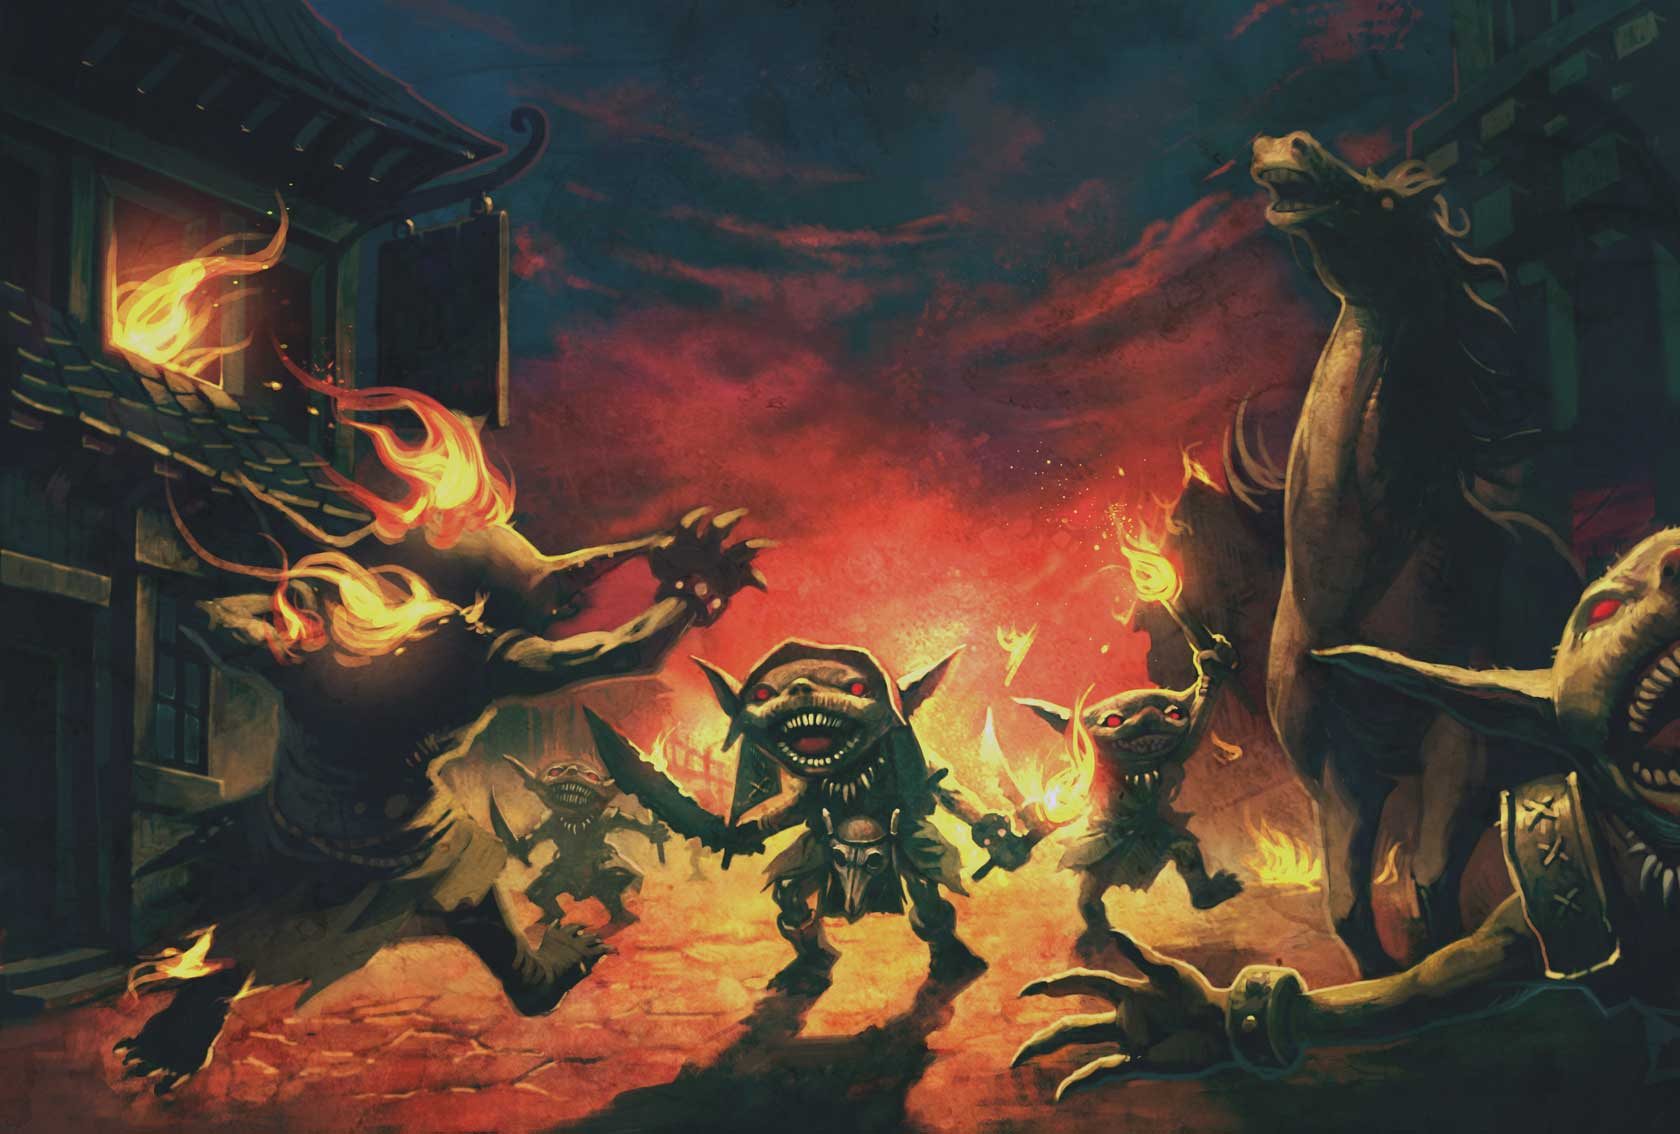
\includegraphics[width=\textwidth]{./content/img/goblin9.jpg}
\begin{figure}[h]
\end{figure}
\end{center}

\clearpage
\subsection{Episode 2: In the Tiki, Tiki, Tiki, Tiki, Tiki Room}

\DndDropCapLine{T}he year is 6653 CC (Church Calendar). In their search for the Stone of Un'thala, the group set off Southwards from Vathos Boundary following the directions given to them by the hunter, Gerard.\medskip

After a day’s travelling the group settle down for the night with Kolo and Pilch taking the first watch. The tension and hatred between the two is palpable and they stare intently at each other. Pilch is briefly distracted, which gives Kolo the chance to disappear. As Pilch desperately searches for his goblin nemesis, Kolo takes the opportunity to attempt to relieve a sleeping Otoria of some of her gold. As he reaches into her pocket Otoria awakes and deals a deadly blow to the goblin, knocking him unconscious.\medskip

Otoria throws the bundle of goblin into his tent, awaking his sister in the process, who mistakenly believes it is her turn to perform lookout duties. She sets down opposite Pilch and resumes the goblin-human stare off. Pilch inquires about Exme’s “gun”, but is not prepared for the onslaught of technical information that Exme is only too glad to discuss. The conversation ends with Pilch being none the wiser, embarrassed by his own vast ignorance. When Exme returns to her tent Kolo has vanished.\medskip

The group push on towards their goal. After some time they arrive at a large skull shaped ice temple that lies across a perilous looking bridge. Exme refuses to enter without her brother and stubbornly resists the efforts of Riphard to carry her along. Otoria takes charge and heads into the temple.\medskip

As the group enter the temple they find themselves in a large spherical chamber, and have their first meeting with the dreaded TikkiTukks™: a race of small bear like creatures with fearsome, culturally insensitive masks. Battle ensues, with the goblins arriving to witness the felling of the final enemy. An investigation of the stone plinth at the centre of the chamber shows that the stone is missing. The goblins remove some masks from the fallen enemies revealing their ghastly faces with sharp, pointed teeth.\medskip

The reassembled group head deeper into the temple in search of the stone. Otoria takes a moment to collect some herbs being cultivated by the TikkiTukks™.\medskip

Kolo unlocks a locked door, which reveals a room full of small boxes that contain some treasure which the group splits up.** Pilch** attempts to reclaim some of the money that he had "misplaced" in the previous session, shamefully accusing the goblins of thievery. Otoria throws him an azure gem to appease him. As the gold is shared out Riphard warns the goblins: “Next time you want your fair share, join the battle at the right time”.\medskip

The goblins attempt to trick another room of TikkiTukks™ by donning masks. Kolo is able to speak in the TikkiTukk™ language. Exme, not knowing of her brothers ability, attempts a bold deception which ultimately backfires when the two are brought to their knees by the devastating attacks from a room full of TikkiTukks™. The group defeat the TikkiTukks™ and enjoy a short rest to recuperate.\medskip

As they continue to explore,** Kolo** pulls Exme back, warning her of a strange tangle of silk threads that hang in a corridor. The group is set upon by a giant spider.** Pilch** is able to set fire to the webbing that covers the walls and ceiling, which keeps the spider at bay, but also traps Otoria on the wrong side of the flames as she delivers her swordy brand of justice. After a short struggle the spider explodes in a mass of ichor.\medskip

Riphard is having gun troubles.\medskip

Continuing on, Riphard activates an ancient trap that fires darts at the group. However, the goblins are not affected since they are of a similar height to the TikkiTukks™; the darts passing harmlessly over them.\medskip

The group manage to fight a large room full of TikkiTukks™, slaughtering their leader (who begins the battle with the glorious war cry ‘tikki tukk doumo arigatou tikki tukk’ ) and claiming his glorious mask as their own. Even with their Tikkitactics and Packtics they are no match for the group.\medskip

Riphard is still having gun troubles.\medskip

The impotent Riphard falls in battle. Kolo kindly revives him whilst pocketing 5 gp, going easy on the man he has no real qualms with yet.\medskip

Further battles ensue. Otaria falls. In a desperate attempt to revive her Exme accidentally punches her in the face, pushing her one step closer to death. Kolo looks on in dismay. Riphard is able to revive her, and the two share a tender moment as he lays his hands on her for “a little too long”.\medskip

Freshly rested the group find a corridor of doors. In full synchronisation, the crew knock down 4 doors only to find, to Kolo’s dismay, more doors inside: “More DOORS. TRICKSY, TRICKSY!!”\medskip

Riphard takes a moment to explore and comes across a fresh water well. He drinks from it and feels the benefits of its cool water, but already feeling 100\% despite the recent battles, does not fully appreciate the benefits the refreshing beverage provides, and so does not share this wisdom with the group.\medskip

The noise of the group knocking/cutting in half doors causes the TikkiTukks™ to bear down upon them.\medskip

Riphard is still still having gun troubles. Exasperated, he makes one last effort and is finally rewarded for his patience and persistence, destroying what once was a young TikkiTukk's™ face in one well placed and devastating shot.\medskip

The group leave one TikkiTukk™ alive to interrogate and help them locate the stone. Whilst passed out, the TikkiTukk™ is tied up and hung upside down. The two goblins don their masks and get ready to intimidate him. Kolo leads the interrogation. The TikkiTukk™ is keen not to die and quickly reveals that the stone is held in the chief’s room. In exchange for the location of the stone of Un'thala, Kolo promises the TikkiTukk™ that he can be the new TikkiTukk™ chief.** Pilch** is also offered as a “sweetener”.\medskip

Kolo is keen to take the prisoner along, but Otoria cryptically states that she is to “have her way with him”. Pilch, greedy for the prisoner’s vitality through his curse attempts to end its life. Otoria is able to block the first blow, but misses the second, which slices open the TikkiTukk’s™ throat. In a cool rage Otoria pins Pilch up against the wall with her large sword and warns him: “I have to work with you, we have shared goals. But you will not do that again”. Pilch is filled with an intense terror at these words.\medskip

The group collect themselves and prepare to head to the chief’s lair to collect their prize

\begin{center}

\includegraphics[width=80mm]{./content/img/kolo2.png}
\begin{figure}[h]
\end{figure}
\end{center}
\subsection{Episode 3: The Horse Whisperer}

The group begin in the bedroooms of the Tiki Tuks after the brutal, and controversial, murder of the "friendly" Tiki Tuk by Philo.\medskip

The goblins, unimpressed with this behaviour and sympathetic to the Tiki Tuks, head towards the treasure room.\medskip

A brief encounter in the water well room see Riphard unsuccessfully attempt to hold Pilch’s head underwater for more details on his violent nature, but Pilch is able to bat him away, swinging his head up in a glorious little mermaid inspired fashion. When asked why he killed the Tiki Tuk, Pilch looks genuinely conflicted.\medskip

Riphard wanders down an unknown corridor, much to Kolo's chagrin. Riphard explains that while Kolo just wants to find the treasure they know about, Riphard wants to find "the treasure that we don't know about”. Riphard is rewarded for his inquisitiveness by finding a stable full of boar and two more Tiki Tuks. Kolo is able to deescalate any possible fight using his language/diplomatic skills, thinking quickly on his feet about an alibi where he is actually visiting his uncle. The goblins laugh at the success of their favourite trick.\medskip

Riphard discovers another large corridor, this one lined with spiked walls and a mossy floor. Exme is able to discern that this used to be a booby-trapped room, however, it has long since fallen into disrepair. However, she does notice the strange fungus growing on the floor and harvests as much as she can along with her brother. Riphard is asked to help, but stubbornly refuses, not being one to do groundwork for such lowly creatures as goblins. Pilch is asked and curiously finds himself accepting the instructions.\medskip

The goblins head to the chief’s rooms. Exme discovers "nothing at all" in a room that she inspects, whilst Kolo recovers a strange, smooth, and intricately engraved stone under a pile of furs in the chief’s bedroom.\medskip

For some reason Pilch decides to argue that this might not be the fancy stone we have been sent here to find. Riphard queries just how many fancy looking stones Pilch thinks Tiki Tuks will have. Exme fumbles through her bag for a while, eventually pulling out a strange device which she passes over the stone. It delivers a small printed out piece of tape in Goblinese which she eyes before confirming that it is indeed the stone of Un’thala. Otoria is not surprised as she feels that most normal stones would not have received such careful treatment and preparation. The goblins inform the group that it is time to sleep, but the rest of the group resist the idea.\medskip

The group take some food from the stores, but are urged by Kolo to leave some for the Tiki Tuks. Kolo also leaves a message saying “nice to see you uncle”.\medskip

Pilch is racist.\medskip

The group travel for half a day, back towards Vathos Boundary, Exme noticeably struggling with her large and heavy bag. The group set up camp. Exme disappears for a short while and returns with herbs that she starts combining with the fungus in a small pestle and mortar. The entire group finds themselves falling asleep.\medskip

During their sleep they share a common dream in which Lazarus speaks to them and congratulates them on their progress so far. He lays out the next challenge, which is to head north to Hope’s Rest. He reveals Pilch perhaps has the closest connection to his kind. He instructs the group that they are to set up base in this liberal township, and will require money and transport to further their interests. The dream fades around the chuckles of Meredith.\medskip

The non-goblins in the group feel weary and drained.** Pilch** deduces that they may be suffering from Zukor’s Rot as a result of being shot with ancient darts in the Temple of Un'thala.\medskip

Exme hands Pilch a single packet of grey paste. She thanks him for his help in gathering the fungus, but berates him for his treatment of the murdered Tiki Tuk.\medskip

The group travel back to town and Otoria begins making inquiries concerning the exploding stable. Kolo and Exme mysteriously disappear. It is revealed that on top of this disaster, the town is now suffering from a spate of horse robberies, including those that led a caravan which is rumoured to be travelling to the north.\medskip

The group visit Black Smith the blacksmith where Kolo, mysteriously reappearing, requests new daggers. Exme, also mysteriously reappearing, attempts to hire the workshop to complete a project. Smith is initially dismissive, however his mind is changed rapidly when offered an ornate, solid gold necklace in return. The goblins begin their work, Exme concentrating hard on her work, and Kolo jumping maniacally on the bellows and hitting things with a hammer. The remaining members head to the titty bar.\medskip

Pilch tries some new, innovative ways of begging - he attempts hawks the Tiki masks as blood money, and gets a free drink from other alt-right extremists, but is told to sell the masks to the captain of the guard.\medskip

Riphard follows the blacksmith home and, once he has gone to bed, breaks into the man’s home and steals the necklace back. The rest of the group is unaware of this.\medskip

The group meet up in the morning and Riphard inquires where to fence sell "totally legitimate jewelry" in the town. He is directed to a jewelry shop where he is given a reduced price for the necklace. Shops have to make a profit, so that is completely normal practice and not a reflection on Riphard's bargaining skills.\medskip

The group head to the city guards offices to inquire about potential jobs and the stable mystery, that isn’t really that much of a mystery when you think about it because it was probably certainly a black powder gang or church related jobby.\medskip

They meet the half orc captain of the guard Urnok and his troll “friend?” Gumshoe. The group discusses local issues and learns more about how they may secure passage to the North.Kolo is a good detective gabrin. Riphard assures people he is a real pastor. Pilch sells 6 Tikki Tuk masks.\medskip

The following jobs are highlighted:\medskip

    Giant boar - Farmsteads in the North offering 50 gp to kill it.\\
    “Jennie’s girls” - Ex-whores who turned to crime after their profession was officially outlawed. Spread like herpes through the empire and can most likely be found to the north. Their leader is a woman called May or “some bitch called May”. The group is told t'arrest her, May.\\
    The SRA - Small Rights Activists. A collection of, mainly, gnomes and halflings who perform terrorists acts in their most-likely justified quest for improving the rights of smaller folk. Leader is Razzle Backshine, a gnome with a penchant for exploding things in people’s faces. Also spread out through empire.\\
    Diego Escabar and his Merry Men - A charming half elf who claims to steal from the rich and give to the poor, but doesn’t actually do the key last bit. Likely located in woodlands nearby. This is a local group.\medskip

Jobs are paid at a going rate of 5gp per severed left ear. Riphard wants to provide scalps, but is informed by Urnok that scalps are too easy to forge. Riphard accepts this explanation, explaining to the group that ears have a unique print, like fingers, which can be compared to the ear-print database the chief almost certainly keeps for this very purpose.\medskip

The gabrins try to turn Pilch in to the guards as Diego, but are unsuccessful. Riphard wonders whether Diego's men would live in a sort-of ghetto, a "robbing hood" if you will.\medskip

Pilch points out that it may be useful to try and recruit these groups, or at least align their interests with our own, and work together against the church.\medskip

Kolo asks Pilch if he has had sex. He replies that he totally has.\medskip

Riphard does not want to arouse suspicion and tries to persuade the group to let him visit the local pastor by himself. After some initial reservations the group allow him several minutes alone before they also insists on seeing the pastor themselves for no discernible reason or purpose.\medskip

Riphard's meeting with the pastor gets off to a tense start. “Are you here to help me?”. “Quite the opposite”. “You’re here to hinder me?”. Riphard questions the pastor on "the inquisition", but the pastor bats away his inquiries as mere tall tales. Riphard attempts to show the pastor proof of the inquisition by showing him the fatal wound he received that sent him to hell, but upon lifting his shirt finds his body shows no signs of trauma at all. The pastor tells Riphard he should ignore these scare stories. Riphard replies that in fact it is the pastor who should not ignore the warning signs. The rest of the group is unaware of this.\medskip

Riphard storms out and walks past the group without a word, looking very pissed off. The group take this as a sign to enter themselves.\medskip

Otoria and Pilch question the pastor, who has suddenly developed a tremendous stutter for some reason, and learn some things about how the Church operates, predominantly linked to their communication channels.\medskip

Riphard looks at boobs, too cheap pious to pay for a touch.\medskip

The group end up in the titty bar where Kolo is able to charm/seduce the busty barkeeper into revealing that she used to know May, back in the day. She reveals that May can be expected to be found to the east of the First River. The lady, flushed with lust towards the sweet-talking Kolo, retires to a back room to cool down. Kolo mysteriously disappears again.\medskip

The group spend a final night in the titty bar before setting off on their next adventure. As they sleep Lazarus visits them again to tell them that now they are in possession of the stone, some members may find themselves more attuned to any pre-existing magical conditions, but that this shouldn't affect their premiums.\medskip

\begin{center}
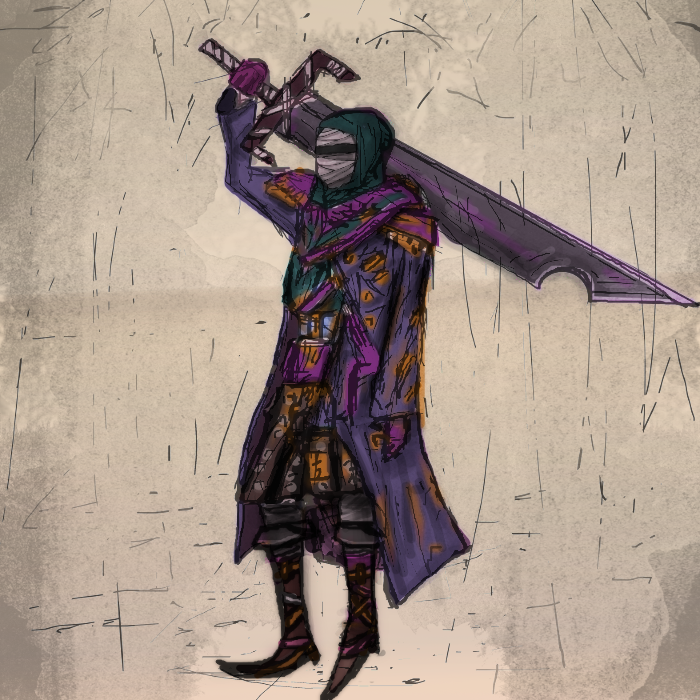
\includegraphics[width=80mm]{./content/img/otoria1.png}
\begin{figure}[h]
\end{figure}
\end{center}

\clearpage
\subsection{Episode 4: Whores or Boars?}

\DndDropCapLine{R}eturning to Vathos Boundary, Otoria and her assorted friends are seeking passage North, and have been given a list of gangs that may have stolen all the horses.\medskip

They wake up in Marcey’s and try to decide how to proceed.\medskip

Otoria wants to infiltrate the Heights Rights lot. Gabrins wants to hassle the Fancy Men.\medskip

Riphard sits in the pub, the Gabrins run off.\medskip

Riphard wants to walk 6 months instead of finding any horses. He sits in the pub by himself to try and achieve this.\medskip

Gabrins and Otoria else goes to see the Blacksmith who’s real sad. Apparently his necklace has got stolen. Otoria wants to find it. They go off to the Blacksmith’s house and look for clues.\medskip

Pilch and Riphard bond.\medskip

CSI:Vathos ensues at Black Smith’s house. Apparently the necklace was stolen by one non-small person. The fidelity of the blacksmith remains in question.\medskip

Kolo looks for criminals to ask questions.\medskip

Riphard is pissed. It’s, like, 12:30. Pilch leaves him to his own demons and goes to wander the streets aimlessly.Then, all of a sudden he discovers something important.\medskip

Meanwhile, or earlier or something, Otoria talks to the police man and he suggests she checks the local jewelers, so see if whoever stole it tried to sell it. She says she’ll have a look.\medskip

Gabrins go into the Mos Eisley Cantena, and talk to a big orc man. Kolo tries to be tough, but is absolutely not that and gets thrown around and nearly thrown out. Then Esme gets involved and is intimidating as fuck. She tries to get the orc man to play cards to win information about the Fancy Man, but that doesn’t work. There’s all sorts of back and forth.\medskip

Then, a “Fancy” Woman appears (not a “Fancy Woman”). She offers to help the Gabrins if they come to their hideout. They say they’re going to gather everyone up and head out with her.\medskip

Pilchard found an old man. He talks to him about how things aren’t as good as they used to be. There’s also not as young a man. Their names are Casper and Germaine. They are woodsmen. He scares them by being a crazy person. There is no inquisition. He asks them if they know any benders. Pilch is a weirdo.\medskip

Otoria finds the jeweler, and the necklace, and the truth.\medskip

Riphard is pissed. Then he’s outside in the alley, propped up against the bins, with Otoria trying to kill him, and then Gabrins trying to steal his money. The Gabrins want to keep him alive, but Riphard himself doesn’t seem to have as much interest in that and tries to shoot Kolo. He misses, and Pilch turns up. Riphard tries to run and is instantly struck down. It’s tragic.\medskip

Otoria starts dragging him to the police station. Half way there she’s convinced to take him the blacksmith’s instead.\medskip

The blacksmith convinces Otoria not to take Riphard to the police, when the group tell him everything, because he would be killed by the church, attracting a lot of attention. Otoria wanted to cut him into little bits, so she’s not super happy about him getting away scot free.\medskip

The group give the blacksmith a shit ton of money, then go back to the pub. Riphard sleeps his pain away.\medskip

Gabrins stack up inside a coat, and everyone goes into the alley to meet the lady.\medskip

The lady is totally fooled by the Gabrins in the coat, for real. She insists on the group helping her or some shit before she tells them where the fancy men are.\medskip

The group head North, out of town, to Whorecity. Then west, then through some hills, then some hillocks. Then there’s a camp. It’s a little bit secret. Otoria and the lady (who’s called Delilah) get on like a horse on fire (like what happened in the stables that time).\medskip

WELCOME TO WHORECITY!\medskip

The group get taken to the Queen Whore, Mae. They brag about their wealth, insult Mae’s fashion sense and then finally get round to actually talking about why they’re there.\medskip

Djago and Mae don’t seem like besties, but Delilah jokes that they are. What’s up with that?\medskip

Exme wants to know what whoring is.\medskip

Otoria wants to know where the horses are. Mae implies, but does not say, that she knows where they are, but says they need to do work for her first.\medskip

Kolo makes a deal. No one’s quite sure what it is.\medskip

Apparently the whores buys their boots in bulk. They’re damn fine boots. We should get some.\medskip

Mae admits the Fancy Men have all the horses, and says she’ll tell them where to find the Heights Rights lot, so they can kill them, and then she’ll tell them we’re the Fancy Men are, so that they can kill them.\medskip

Otoria tells Mae not to tell anyone they’re there. Esme tells Mae that they’re terrorists planning to take down the state.\medskip

Everything seems fine.\medskip

Mae has work to plan.\medskip

The gang manage to get two horses, and squeeze on to the back of them.\medskip

Riphard gets hit on\medskip

They ride horses to Razzle’s house. Razzle is king of the Height Rights. This is his house.\medskip

Gabrins are going to go in first, like they’re HeightRightsers. They’re going to see if they can find Razzle, and then come back and do some Strats and Tats.\medskip

Gabrins enter HeightRightsManor.\medskip

There’s a fucking hobbit.\medskip

He’s going to fucking whistle like a bellend.\medskip

The Gabrins shout at him and introduce themselves, to get ahead of the scandal.\medskip

The fucking hobbit’s called Nickles.\medskip

“Big rights for small people”, says Esme.\medskip

The Gabrins tell Nickles that they’ve been persecuted for being little. Kolo has terrible flashbacks to the Cantena. This pleases Nickles and they get taken inside.\medskip

I can’t really see what’s going on any more.\medskip

There’s a sleeping area and some stairs.\medskip

Here’s Razzle. He’s a gnome. He’s got a big bag of fireworks. He’s stressful to listen to.\medskip

He’s a little leprechaun gangsta, see.\medskip

He wants to burn Djago down, see.\medskip

Esme tells everyone about wanting to bring down the church again. Razzle wants to kill humans indiscriminately. It’s a debate for the ages. Only Razzle can use the boomstick.\medskip

Esme’s, like “please”. Razzle’s like, “NO”.\medskip

Esme offers information about booms, in return for… a thing… or… anything. Hundreds of short people will die, but I think that’s the plan. I really don’t understand. It definitely sounds like they’re not going to kill this guy.\medskip

Razzle wants Gabrins to kill whores.\medskip

Razzle wants to be quiet and small. He’s failing at half of that.\medskip

Kolo wants to pick up part time job killing humans, Esme thinks they should focus on taking down church, so that they can kill even more humans.\medskip

Gabrins suggest Razzle should come with them on mission to kill whores. Razzle says no. He sends his best men, though.\medskip

The Gabrins and the best men go out into the woods, where the Bargins plan to kill them. Otoria and Pilch talk about when to kill everyone.\medskip

They eventually decide to wait until everyone’s asleep.\medskip

In the woods, everyone’s asleep. Time to die.\medskip

Pilch tries to back out of this whole thing, trying to get the Whores and Height Right’s to be friends.\medskip

Otoria wants to cut off their tongues and hands.\medskip

Esme is spread the gospel of The One, trying to convert the Best Men. Esme and the Best Man (who’s a woman) take a minute and pray to The One.\medskip

Everyone else is hanging out in the bushes.\medskip

Everyone suddenly doesn’t want to kill them any more. They feel really bad for the small people, but then they kill them anyway.\medskip

There’s a brutal massacre.\medskip

Everyone decides that they’re going to kill Razzle, but that they want the small people to be free and happy under a new ruler.\medskip

Everyone gets back to the cave and prepare for shit to go down.\medskip

TO BE CONTINUED...
\subsection{Episode 5: Pitter Patter of Tiny Bears}

[The following pages are torn from a larger volume, and hastily rebound with string - One corner is singed implying someone attempted to burn this or the entire volume.\\
The writing is in a quick, hurried, but practiced hand, and the type-face changes occasionally as though the writer grew bored of their style]\\
Codenames as follows...\\
- SH - Shadow Hound - Yours truly\\
- RP - Righteously Pissed - the drunken dwarf\\
- JR - Jilted Royal - the foreign lady\\
- SR - Shifty Rogue - the thieving goblin\\
- JM - Joyful Mechanic - the inventive goblin\\
\DndDropCapLine{S}o we’re in a cave, and just slaughtered a small number of small folk to whom we hope to ally. Great.
SR has initiated a plan to take over the small-peeps by killing Razzle, SH says we should try and discredit the small folks leader (Razzle) - Seems that the goblins and Dwarf are going to go in and try to convince everyone else that he’s gone rogue and isn’t part of the organisation anymore.\medskip
I’m loath to split the party, but the tiny bigots (...small-ots?) probably won’t like me or JR walking in - maybe we can be guards or sympathisers?\medskip
Anyway, I do the honorable thing of burning the bodies (and taking 5 ears), and then forging a document for RP -
"Razzle is accused of collusion against the SRA with his Ofecal Cherch Buziness."\\
We stop outside, and finalise the plan - is as above, but the goblins will go in shortly afterwards to make it seem they were (recently) ambushed.\\
RP Successfully enters the camp, thanks to the forged letter. The goblins sneak in after. RP manages to get found as an imposter, despite the letter. He did not know the secret Nichols handshake.\\
A fight breaks out between RP and 3 members of the SRA - but he’s quickly subdued.\\
Everyone decides to scapegoat RP as a church-worker, still to discredit Razzle. Goblins sneak in.\\
SRA becomes SRM - suddenly, because RP.\\
Goblins come in, pretending to be injured - leant huge credence by my amazing disguising. Two of the SRA fall for it.\\
RP gets blown up. Probably. Razzle likes bombs. “No dwarfy… I expect you to die!”\\
RP starts whipping people. He gets knocked out.\\
Team gobbo and 2 of the SRA run in. One gets blown up, the rest like Razzle more for this.\\
JR is very noisy, it messes up our stealthiness.\\
SH becomes a rock.\\
I get RP back up by punching him, and then dance like my life depends on it (which it did).\\
RP is then useful by disarming Razzle.\\
Razzle Shanks me, but the shadows protect.\\
The JM Blows off Razzles head.\\
SH, RP and JR (who had been doing pull-ups the whole time) leave.\\
The goblins appoint “Buttons” as the new leader of (this faction) of the SRA.\\
There's maybe 4 SRA left.\\
They also loot: Signet ring (with stampy well) 10 rockets 10gp\\
Papers - Bits of communication, Old Plans, Promotional Material, rambling letters,\\
I’m not happy about this.\\
We rest up.\\
Kolo and Otario have a heart to heart.\\
We all go to see Mae. JR takes point in the conversation. It’s interesting. Mae and Delilah plan with us to go kill fancy-pants.\\
I’m on a horse.\\
Mae gives us 3 people to go take on Fancy-Pants, Diago. One is an Battle-axe barbarian type, others a Crossbow-marksman, as is Delilah.\\
JR and JM also get fancy “dutty ho” boots.\\
On the way (to Diago) we encounter a man that tells us about the giant boar. Delilah flirts with RP for some reason.\medskip

JR - with her Mechanism Bow, JM and SR decide to attack at ranged, and take out the boar slowly.
In the forest, we get attacked by dropbears.\\
RP gets ripped hard. JR flails.\\
Me and the goblins kill nearly everything.\\
The crossbow whore (Martha) dies.\\
I save RP.\\
I get Martha’s Xbow.\\
Wait, shit… I better burn these pages - safer than leaving a paper trail... \\
\begin{center}
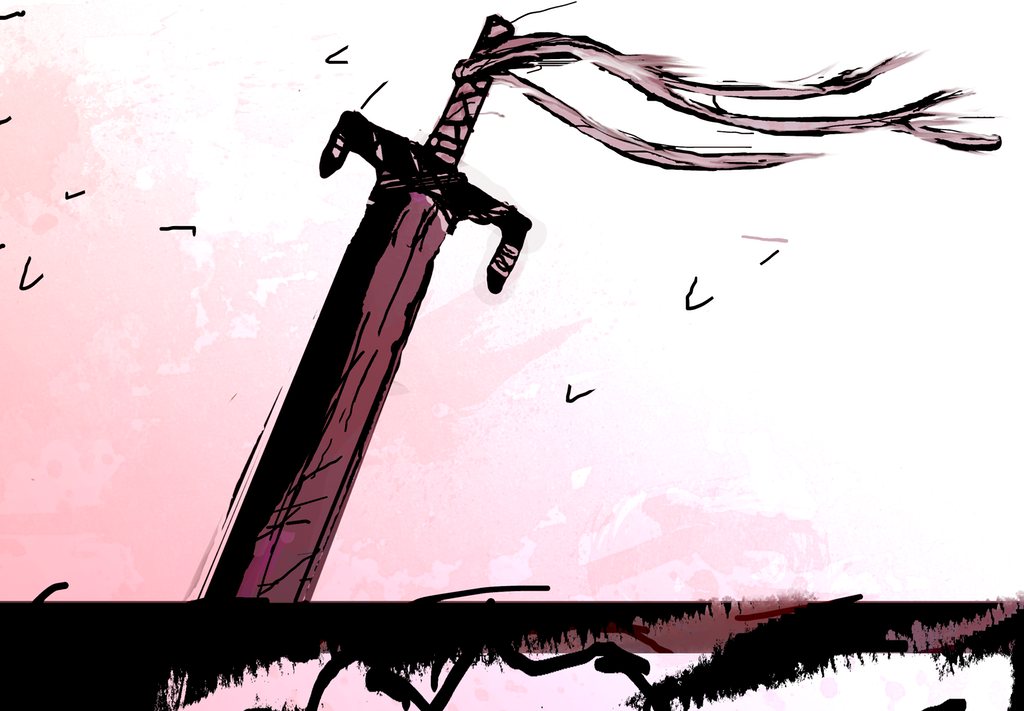
\includegraphics[width=80mm]{./content/img/otoriagrave.png}
\begin{figure}[h]
\end{figure}
\end{center}

\clearpage
\subsection{Episode 6: Arbitration}
\DndDropCapLine{D}ay starts well as we are unmolested\medskip
Pilch talks to Delilah about other men and how to lure them in, he is very keen even if it means traversing vast tracks of forest. Even the Dutty Hoe isn’t willing to put out that far.\medskip
Camp is made, no one wants to sleep, perhaps everyone is super excited about meeting the giant pig. Kolo gets bored and falls asleep.\medskip
Fishy loses his bird, Kolo helpfully brings it back, but it somehow escapes. I am intensely interested in how the bird works, could be proper useful to have a scout, and something to distract enemies in a fight……\medskip
Fishy will pay for this, but first I follow Pig Smells.\medskip
Otario and I go for sneaky first kill on Pig, which is followed by a sudden tactical climb into a tree. Otario winds up and pitches the Gabrin Fast Ball Special. Negotiations unfortunately fail, and after bouncing off the pig… watches as the Strange One leaps and pirouettes onto the big piggy before spanking it with her giant sword.\medskip
Exmeh then lines up a shot and whispers "This little piggy went to market" before dispatching one baby pig.\medskip
Before suddenly there are two Exmehs, wandering about. The Evil twin Exmeh then kills poor little piggy No 2.\medskip
Riphard blows Big Pigs brains out everywhere, no more piggies.\medskip
“It is Impossible to have a Cake and Also eat a Cake” Strange on is Strange.\medskip
Barbeque pork all around, as Pilch adds to his ear collection. Big Pig is Too Big except for fatty hoe who eats most of pig. Impressive…. Riphard is strangely not interested in pig.\medskip
After camping overnight in the pigs den, we move on to through the woods following filthy hoe Delilah. Somehow she knows where fancy man lives….\medskip
Pilch watches Kolo taking a massive smelly pig sized shit. About half way through, kolo turns and make eye contact while pinching off the end of the loaf.\medskip
Pilch is confused about horses and dirt hoes.\medskip
Its agreed that all ravens will now be shot.\medskip
Pilch is a huuuge fiilltthhhyyy liar, about where the enemy are and what they are up to.\medskip
Otario leads the lady charge, to entrap the fancy men. While we sneaky for horses, except Riphard who walks into the camp bringing the good news of the lord.\medskip
Things go well with the fancy pants, as Otario works her magic\medskip
Kolo horse whispers with his own shit, and as he is tying up the horses, stoooopid Exmeh sets off a fire work. Otario then starts a song and does the dance of her people, it is not impressive.\medskip
Exmeh stands statue of liberty esque holding a boom stick high.\medskip
Kolo sets off a horsey train through the camp. “ A sudden Rampage “\medskip
One bandit does his best to salve the horses, “I’ve got this lads” by running in front of them all, who then savagely kill him.\medskip
Otario gets Axed a lot of questions, while pilch hides behind a tent and tries to convince the fancy men their leader is a nerd. Riphard starts a loaded sermon. Exmeh sends some redundant technology burning some poor fuckers face off, before hiding behind a tent!\medskip
Pilch finally finds his ball sack, no correction he hides behind another tent before trying to reason with the enemy again. Luckily he is saved by the tent catching arrows. Strange booyagh is afoot as voices from the forest, as the horses speed out of the village.\medskip
Raven hunt is going very badly, something is definitely up with this freaking bird. Its naked.\medskip
Pilch somehow convinces half the archers to go to bed, while he gets nailed by Capn’ Fancy Pants, and leaking smoke.\medskip
Otario is taking a nap on the table, while Pilch makes an ill timed verbal foray against Capn’ Fancy Pants, and as he pulls out his knife his chest explodes across across pilch from Exmehs rail gun.\medskip
Riphard finally deals with the pesky Axe man, blowing the back of his head out.\medskip
Sterling doesn’t make the cut because Kolo makes the world a better place with one less asshole. Pilch cuts more ears from Diegos Boys, chopping Diegos head off for good measure.\medskip
Otario rides off into the sunset badly, Delilah suddenly decides to stick with the party. Possibly because of sexy smelly gabrins.\medskip
Pilch gets some hot whispers from mega Hoe.\medskip
Return to sender, to find some poor mug still getting a shoein.\medskip
In the middle of town we discover a plate armoured individual standing over a leather clad man. She is holding a gun to the mans head. The gun is bigger and badder than Riphards, giving Riphard a massive Hard on.\medskip
Kolo shits himself, Otario tries to take the hit, but then Riphard out of nowhere gets the game on with the Arbiter! Truth will come and Justice is serverd liberally with a massive sword.\medskip
Otario and Riphard are totally outclassed. Otario gives a long winded speach to the crowd, while Pilch is gone, and the Gabrins are at the titty bar. It doesn’t quite go the way she planned. Not even able to take out a wooden pillar afterwards. She then stalks the scary arbiter woman.\medskip
Riphard gets some top tips from the Scary lady. Otario gets a letter for 500 gold from Arbiter Kyross, which she lets drop to the floor to be cashed at Rivers Falls.\medskip
Riphard gets a note, recommending him to the master at Rivers Falls. To train him up with ninjas. The idea of training with the Ninjas makes him cry. Its genuinely touching. He also pockets the 500 gold note.\medskip
Otario continues to stalk Lady Kyross, throughout the day and night.
\subsection{Episode 7: Mysterious Incident of the Cow in the night}
\DndDropCapLine{P}ilch is the anonymous Jackalope, also in attendance is Anonymous Hippo and Anonymous Frog\medskip
Hester is the owner of the caravan\medskip
Otario is found in the town still staring at the kebab ladies house. He agrees to meet everyone at the main square for departure. In the mean time Otario pays a small urchin to send a letter everyday to convince the Kebab lady that she is still watching her\medskip
At the caravan Kolo is upset that everyone has a caravan except for him. Exmeh locks him out. Pilch cosies up to Hestor\medskip
Boamos under represented caravan member that Otario befriends. He is from South West Africa, which no one has ever heard of. He is happy to help learn Otario. “Otario learns horsecraft” its super effective.\medskip
Riphard and Delilah are having a muffled “conversation”\medskip
Kolo pissing into Exmehs caravan, before running off with tongs and a crucible.\medskip
Pilch looks for some general information, specifically against the church. Exposition dump, nothing out of the ordinary other than that constant war with the minons of the (Valkaar) VARG, and those from Lindedorf who are striking back at the church.\medskip
Caravan People Consist of:\medskip
Leader: Hestor\medskip
Guards: Leorable, Dukey, Dallius, Job\medskip
Merchants: Boamos, Tillie, Sabina, Maarah, Sidney\medskip
Troubles in port AbbeyDale in the East, more people from Masooda, Far to the East across the Ocean. Masooda and NanDuan are not friends.\medskip
Story time commences, involving Drop Bears and changelings….\medskip
Changelings are revealed by throwing salt over their right shoulder...\medskip
NanDuan has a plethora of sand daggers\medskip
Otario makes friends with a horse, before …\medskip
Kolo goes off for a stealth investigation\medskip
Pilch is caught spooning Hestor\medskip
Fierce discussion takes place about what to do about the ambush. Pilch wants to hide in the, kolo is a fan of stalking the beast\medskip
Pilch has not romanced Hestor after all.\medskip
Hoof prints are massive, but its super light on its feet.\medskip
Probably one of the Nanduisian Balloon Cows\medskip
Otario and Kolo join forces and become Super Mega KolOtariozord, its is not supereffective\medskip
Everyone runs blindly into the woods, some more blindly than others\medskip
Otario prepares the bey blade, but to no avail as she is booted out from underneath kolo, but what is not a flying cow afterall.\medskip
Pilch runs away leaving otario and kolo to die. Luckily the Leucrotta is slain by Riphard awesome boom sticks, and the cross bow bolt of a returning Pilch.\medskip
Exmeh fixes up the axle of the lead wagon and the party moves onto RiverFall which is beautiful.\medskip
In the middle of which is a large church, the sanctuary of Novetta.\medskip
The spire of “emoticon” -Imota Kan\medskip
Riphard hates women\medskip
Armor is expensive
\subsection{Episode 8: Freaky Fishy}
\DndDropCapLine{A}s we join our “heroes”, they have just arrived in the town of Rivers Run or something. It was a long night, so a nice warm burrow was dug for Pilch to enjoy. Pilch lives in a hole in the ground.\\
This town that they’re in is where the church lives.\\
People really want Otoria to stop dying so much and actually help, so they’ve all gone to the shop.\\
They can’t afford any armour, so try to find work to get money. Apparently there’s trouble a’ mine.\\
There’s a bunch of other places to go too.\\
And 4 taverns. Rip gets hard.\\
Sad Crusader, Club and Cask, Open Flask, Minstrels\\
Sanctuary of Novotel - Church place to gain power and money\\
Everyone goes to the Sad Crusader, obvs.\\
It’s great. Everyone has a good time and the service is great.\\
Kolo burns the raven.\\
Pilch drinks terrible beer and Kolo drinks some Killepitsch shit.\\
Kolo buys some of it and some matches. There’s no explanation for this at all.\\
Pilch goes wrong somehow and starts rolling around in his own vomit.\\
Everyone decides it’s probably for the best if they put him down, which is sad, but unavoidable.\\
Then Pilch shits magical darkness and Kolo sets fire to the pub in response.\\
Everything goes to shit and people are running through walls and shit.\\
Outside, everyone realises Pilch is possessed or something and start taking him to the river to drown.\\
Otoria realises there’s two old men trapped inside and runs back in to save them. It’s awesome and she picks them both up and bursts out through the wall of the burning pub.\\
She then returns to the rest and helps them throw Pilch in a river. Kolo’s been rolling him, which is cool but not that efficient.\\
Pilch immediately starts drowning. Everyone’s “really upset”.\\
Pilch wakes up and gets out, then he and Kolo mud wrestle for a bit.\\
The fire’s really getting going now, most of the crew help out, Riphard runs off to another pub, Munchkins, the suave place.\\
He doesn’t get let in, because he’s not cool enough, but then he does the classic Inspector Routine, and totally bosses it.\\
He’s in.\\
Everyone else is saving lives and property from that fire they started, but whatever Riphard, you do your own thing.\\
Munchkins is like that cool jazz bar in Spiderman 3.\\
This whole sequence is basically just Riphard’s methdream. Everyone keeps giving him compliments, booze and boobs.\\
Meanwhile, at the disaster zone, the brave volunteers have sated the fire.\\
Otoria gives the man some money for rebuilding the pub and Kolo asks him to come with them on the adventure. He declines, but gives Kolo the recipe for the Killepitsch stuff.\\
Otoria and Kolo take Pilch off towards the Spire of Emoticon/Immodium, apparently Kolo knows some secret Gabrin magic to fix Pilch which seems to involve leaving him in a hole in the ground and leaving.\\
Riphard is 13 shots down. The remaining 7 shots get put in 2 cocktails for the road, and he crawls off to the central church place to report in with what he found from drinking all of this bullshit. It takes him hours.\\
He’s greeted by two guards, he tries to make them drink the remaining cocktails, and then forgets he’s not a female arbiter. Somehow he gets let inside.\\
He’s going to meet the guy who’s supposed to give him all the money. Everyone’s being nice to him, despite the fact he’s a fucking mess.\\
Riphard meets the guy. Gendry goes and gets the money.\\
Riphard tries to hold a conversation. It goes as well as you’d expect.\\
The guy makes him undrunk. He gets nuzzled.\\
Riphard puts his hand on a ball and it tells him his destiny. His destiny is to be an Alligator.\\
The guy tells Riphard to go and pray at some artifact at the Spire, which is run by the guy’s daughter.\\
Gendry does some top-shelf slapstick with a big sack of money.\\
Riphard takes his comical bag of money into town and looks for somewhere to hide it. He goes to an old man’s shit brick house.\\
The old man thinks Riphard is here to put him down. He’s mildly upset about this, but seems to think his daughter would approve.\\
He’s so old.\\
SO OLD.\\
SO LONELY AND SAD.\\
His daughter wants him to die, because she lives in a wooden house.\\
Rip goes off to find a hiding place for his huge bag of gold. I think he’s going to kill this sad old man.\\
He tells the old man that the gods want to run a shop in his house. The man loves this idea.\\
The old man decides to leave his house to the church when he dies. Riphard is definitely going to kill him now.\\
The old man’s name is Derek Bobacious.\\
Riphard goes off the get himself written into Derek’s will. Hero.\\
Kolo and Otoria are digging a hole in the woods. Otoria finds out that Kolo’s planning the kill Pilch before they bury him, and she doesn’t like this. She convinces him to take him to the Spire instead and they ride off.\\
Back in town, Riphard’s got the contracts drawn up, meets Delilah. He decides to take her to meet Derek.\\
Derek gets the will and sexually harasses Delilah.\\
Derek boasts about his old man dick.\\
Riphard opens a bank in Derek’s house. He calls it Northern Rock, because it sounds sturdy and dependable.\\
Derek reveals that his actual old man dick is broken, but the old man dick in his mind is doing just fine.\\
Riphard sets everything up and rides off to meet the others.\\
They arrive at the Spire.\\
They meet Holly. She lets them in.\\
There’s a party going on, but they’re not invited, especially the definitely naturally ill guy they’re here to find a cure for.\\
Riphard presses Holly for info about the vaults and shit.\\
He tries to get investment into a colab on this banking startup he’s planning.\\
Holly tells them where all the books they want are, and also that only Pilch can read the ones on possession and Devil shit, which why would they even need that, because he’s just got food poisoning or something.\\
Riphard finds a book about the thing he’s looking for. Otoria finds a book about syphilis. Kolo finds a book about possession and what to do about it.\\
We need to get a pastor to do a thing and then purge him.\\
If this doesn’t work, we’ll just kill him.\\
We’re gonna fix fishy,\\
Riphard is chanting, Kolo feeds Pilch half a bottle of Killepitsch.\\
Vomit.\\
Vomit. Vomit. Vomit.\\
VOMIT.\\
VOMIIIIT.\\
VVV OOO MMM III TTT\\
It seems moderately successful. Fishy lives.\\
He gets a shadow sword, and stops being so obviously possessed.\\
Pilch agrees to stay at least 15 feet from Otoria at all times he's not actively saving her life, on pain of sword.\\
Everyone goes to a party.\\
There’s all sorts of people at the party, including people from the same continent as Otoria, which is rare.\\
Otoria introduces everyone to a plant expert, and goes off to get drinks.\\
Holly turns back up, and offers to show Riphard the artefact he’s here to see. The others can come too.\\
Pilch puts a sword in his ear.\\
Rip, Kolo and Esme go to see the thing.\\
Pilch goes to be sick in a hole.\\
No one realises that the last time they saw Otoria, she was off getting them drinks.\\
Everyone else is in the vaults, having a lovely time all together.\\
They go and see the thing. It’s a ruby sphere 2 fists wide.\\
Mike loves getting fisted.\\
Riphard meditates into the stone. He realises he loves the church loads.\\
Suddenly, off in the distance, some people hear a scream, most people do not.\\
TO BE CONTINUED
\subsection{Episode 9: Live Free or R.I.P. Hard (In loving memory of Lady Otoria Hearthrust)}
\DndDropCapLine{T}he screaming continues.\\
Holly: “what what whaaaa?!”\\
Holly runs to the door: “Leroyyyy mmmmmJeeennnnkinnnnsssss”\\
The group crowds around the door. Clanking machinery and voices are heard in the distance\\
Man 1 “Tony, we need to break the door down quickly.”\\
Tony (probably) “Don’t worry, she knows what she’s doing”\\
They don’t know the doors are unlocked to this super secure facility.\\
Esme is confused about everything.\\
We open the door and see 3 stunned figures outside the door: burly black man (Theo), half orc (Tony), and Eastern looking lady with daggers. They draw their weapons.\\
MEANWHILE\\
Otoria explores the upper levels carrying around the 3 drinks she got for the group. She reflects on the peace and quiet: that is never a good thing. She hears heavy footsteps bound up the stairs.\\
Otoria freezes and watches the doorway to the stairs.\\
Man 3 “Round up the others. Take care of the hostages, right Alexander?”\\
Man 4 (gruff voice) “Don’t tell me how to do my work.”\\
Otoria approaches Alexander and scolds him for mistreating Man 4.\\
The men note Otoria’s notable weaponry and draw weapons.\\
MEANWHILE\\
Exme is fucking on it and pops a shot off first. She misses.\\
The dagger lady “eyes up Kolo” and waits. Lustfully.\\
Tony gets a glancing spear blow on Kolo (more innuendo).\\
The dagger lady now stabs Kolo for some reason who cries out for Exme’s help.\\
Everyone misses everyone else.\\
MEANWHILE\\
Otoria gets wet for some reason.\\
MEANWHILE\\
Pilch tries to use his new sword. He sucks as expected. He tries to retcon it with luck, forgetting AGAIN about his raven that magically gives everyone advantage. He now magically hits here for minimum damage, giving her the equivalent of a paper cut. Some magical extra damage comes out of nowhere and she explodes. That’s a bad paper cut.\\
MEANWHILE\\
Alexander tries to spear Otoria and bang her (... come on). He fucking rapes her (not litereally). Otoria is in bad shape.\\
Otoria respond with a fancy sword swipe. It’s pretty fucking fancy. The men look impressed and injured.\\
MEANWHILE\\
Riphard talks to his bullets. For 6 seconds. You’d have thought he could manage more than that, but no.\\
Exme kills Theo.\\
“Frank” (Tony?) takes Holly hostages and backs away threatening to kill her if we move.\\
MEANWHILE\\
Otoria continues to battle the two men without dying, which is an improvement.\\
MEANWHILE\\
Pilch thinks about taking off Holly’s clothes. Very inappropriate for an unconscious hostage. Probably telling of his character. Pilch does something involving magic. It didn’t seem important.\\
MEANWHILE\\
One of the dudes tries to bang Otoria again, but misses so badly he makes it super easy for Otoria to stab him. Otoria misses. But in her miss scares the fuck out of the men. They literally shit their pants. Then she remembers she actually had advantage and they retroactively take damage, probably from the pant shitting. The guy drops his weapon.\\
MEANWHILE\\
A large inky black void has surrounded the doorway, pilch, and the hostage situation. This is probably Pilch’s fault.\\
Riphard says “Fuck this noise again” and pats Kolo on the head 10 times.\\
Exme and Kolo looks at each other and realise their opportunity. A vault full of invaluable secrets, during a robbery, with the keeper conveniently unconscious and subdued.... It would terrible if some of the items went missing.\\
Exme uses her identify machine, but it beeps confusedly at her. She walks off.\\
Frank (the girl was Tony all along) panics and drops Holly in the black shit mist. He runs in the direction he thinks the stairs are in.\\
Kolo runs into the black shit mist for some reason. He trips over Holly and falls on his face.\\
MEANWHILE\\
The lady tries to stab Otoria… and misses. The battle rages on.\\
MEANWHILE\\
Pilch reabsorbs the darkness into his ass. He approaches Kolo and offers him a hand to his feet. Kolo thanks fishy.\\
MEANWHILE\\
Alexander runs off allowing Otoria to stab him. She misses. Otoria tries to intimidate the already scared man, commanding him the halt. He stops. Fucking Jedi shit. Otoria then swipes at the lady and she’s barely standing on her feet, crumpling her breastplate.\\
Riphard commands the running man to DANCE! He stops and starts dancing, telling the others to subdue him.\\
Exme is homing in on something and finds a small ring.\\
Frank continues to dance aggressively and sexually.\\
Kolo wants Pilch to throw him and jumps into his arms.\\
MEANWHILE\\
The lady tries to stab Otoria again. Misses again.\\
MEANWHILE\\
Pilch runs with Kolo and throws him at the now stationary and non-dancing Frank. Pilch uses some kind of homing device and bullseyes Kolo into Frank’s face.\\
Kolo does a barrel roll in the air and headbutts Frank while stabbing him, knocking Frank out cold.\\
MEANWHILE\\
The mighty battles draws to an inevitable conclusion. Otoria does some more unnecessary. fancy sword shit and opens some sardines. She cuts the ladies face off and struts towards the still terrified man.\\
“Everything went much better for you because you did what I say. It will continue to be better for you if you continue to do what I do. Tell me everything”.\\
The terrified man spits blood and tells Otoria that they were robbing the place (no shit).\\
Otoria wonders if the man parties. He does. He tells her they took the party people hostage. He says they didn’t want violence, despite rushing Otoria immediately on sight. He said she looked like a badass. Otoria tells him to go to bed and rethink his life. Settle down. Get a job. Contribute productively to society. He agrees to have a nap and try to figure his life out. Otoria breaks his spear and lets him be.\\
“By the way, never seen a woman fight like you.”\\
“I am Otoria Hea…”\\
“LET ME FINISH…. Except for Lark”\\
“Thanks for the cryptic clue.”\\
“No, you already know who that is. The blonde asian lady.”\\
“Ohhhhh yeeeaaaaah.”\\
MEANWHILE\\
Riphard practices his bondage techniques, convincing the others not to skin the man.\\
Exme quickly works out how the fancy 17 lock door works for Riphard.\\
Kolo agrees to guard the treasures (yeah….).\\
The group take the unconscious Frank and now-conscious Holly to the security HQ within the tower, which is apparently just the guards at the door.\\
Riphard explains to Holly about the robbery and non-so-subtly implies the need for a reward.\\
The guards, who have no fucking idea what’s going on at this super secure treasure tower, inquire as to what’s going on. Pilch tries to explain to the guards what’s happening despite all this being Riphard’s idea. Who is oddly quiet, scribbling notes, probably about their lax security procedures.\\
It turns out that the 2 guards are part of the robbery. This explains a lot. Riphard takes notes harder. “TRUSTWORTHY GUARDS!!!!”.\\
Riphard quick draws his pistol and shouts “THUNDERCUNT!” and shoots one of the motherfuckers.\\
Kolo hears the distant rumble of Riphard’s gun. Exme does not.\\
One of the guards doesn’t hit Riphard.\\
Pilch drops an ear (wtf) and further confirms himself to be very much a Stephen character by looking for the best way to run away. He contemplates jumping into shit to surrounding himself with matter similar to himself. Holly and the unconscious half orc block the corridor. Pilch stabs the unconscious half orc to Riphards confusion.\\
Riphard misses with his whip.\\
The men stab Pilch in the face with a greatsword and miss with another.\\
Pilch tries to actually do something useful and stab the dudes (totally after sending the Raven out for advantage). AND MISSES LIKE A CUNT.\\
MEANWHILE\\
Otoria eats some grey goo, totally oblivious to the thunderous blast from below. She decides it’s party time and descends to the party room.\\
The group uncover the mystery of Imota Kan (NAKATOMI BACKWARDS OMG) and it turns out the whole thing is a Die Hard rip off. Pretty sweet. All the dudes are named after the Die Hard people too. Fuck. Does that mean it’s Christmas?\\
Hans (come on) cuts a guy's head off as Otoria enters the room. Everyone starts making Die Hard references.\\
Otoria banters with Hans. There’s a lot of talk of mess and shit shows. No one likes mess. Hans explains he’s here to rob the tower (YEAH WE GET IT). Turns out Hans threw the party in his own honour, what a cunt. The conversation goes on for a while in true hollywood style with the villain fully explaining his plan for some reason.\\
Otoria tries to convince Hans that his men in the vault are dead. Hans proposes a bet to see who’s dead.\\
MEANWHILE\\
Riphard starts singing Firework by Katy Perry, who totally exists in this universe, inspiring Pilch and Holly.\\
The evil dudes miss.\\
Pilch kills a motherfucker and kicks him off the bridge.\\
Riphard fucking whips the other dude’s feet, who entangled in whip stumbles off the bridge to his grizzly doom. Wilhelm scream\\
MEANWHILE\\
Otoria notices Kolo and Exme sneaking out from the all too convenient poop-chutes-come-ventilation shafts. They now know what it’s like to be TV dinners… after they’ve been digested, shat out, and flushed away.\\
The hollywood conversation continues. Otoria tries to walk away, but the henchmen fire their crossbows at her, but all miss leaving an Otoria shaped arrangement in the wall behind her.\\
Exme left a crate conveniently in the party hall last week, which now starts beeping and humming.\\
Kolo looses an arrow at a henchman, killing him clean. HEADSHOT. His eye extends out of his face on the end of the arrow. Gross.\\
Exme takes a shot at Hans and wounds him.\\
Marco (a henchman) hits Otoria with a bolt.\\
Pilch and Riphard don’t put two and two together, and thinking the job is now done saunter back off into the building at a leisurely pace.\\
Kristal stabs Exme.\\
Otoria does a combat roll on the spot instead of just turning around like a normal person. She sprints towards Hans with the her sword held out in front of her and completely misses Hans.\\
Kolo gets hit with an arrow.\\
Some lady with a katana slashes Otoria while she clumsily runs at Hans.\\
Kolo misses terribly with a poison arrow.\\
Exme action rolls away from Kristal, shooting her to pieces all over a nearby hostage, then dodges a bolt.\\
Pilch and Riphard hear the distant sounds of battle and start sprinting towards the stairs like the brave men one of them is.\\
Hans goes mental at the sight of his dying men.\\
Otoria slashes some people.\\
Kolo gets his with another arrow.\\
Lark (the one with long blond hair) starts singing a song of focus. It sounds like a BabyMetal ballad.\\
Kolo breaks out a DISTILLED poison arrow, and finally kills his tormenter.\\
The forgotten whirring crate finally does something, and falls open. A small roar emanates as a small mecha-bear appears from the dust. It’s super cute. Exme looks surprised in a motherly way.\\
Exme shoots another henchman and fucks him right up. He dead. Exme inspects the mecha-bear, which starts doing a little excited tippy tap dance for her. Everyone’s heart melts. Except Exme, who looks unmoved, the heartless bitch.\\
Pilch finally appears from the stair well. He does a ranged attack for a pathetic amount of damage to the singing lark.\\
Riphard enters and grabs his pistol he had stored behind his head in his hood, totally like out of Die Hard. GET IT? He shoots Lark for much more damage than Pilch, but she still singin’.\\
Otoria dies hard. As usual.\\
Lark, angry at being shot twice, runs at Pilch and Riphard and swipes at them. Riphard gets hit hard.\\
Kolo continues to use his fanciest of fancy arrows and fires at Hans, wounding him badly.\\
The mecha-bear adorably bounds towards Hans, falling over as he does so. AWWW.\\
Exme then fires at Hans, but is distracted by the sickeningly cute mecha-bear.\\
Pilch fucking grabs Lark like a full on rapist and/or Donald Trump. He moves on her like a bitch, suplexing the bitch down the stairs over his head. She’s still fucking singing though, amazing.\\
Riphard runs over and touches up the unconscious Otoria. As usual.\\
Hans tries to stab a prone Otoria, but resembles someone playing a larger hand-knife game, stabbing between her splayed limbs. It’s actually quite impressive. A smattering of applause breaks out.\\
Otoria gets up looking angry. She mightily swings her greatsword at Hans, right at his crotch. It turns out Hans is wearing a very elaborate cod-piece and he laughs, unfazed and unhurt. Otoria runs away. Hans tries to swipe at her, but she’s too nimble.\\
Lark says something at Pilch in Forin. “DIE PEEG”. This is actually seamlessly part of the song. She double slashes Pilch who dies. HARD.\\
Kolo lets out more of the fancy arrows at Hans, who’s still standing.\\
The mecha-bear approaches Hans and gently tugs at Hans’ pantaloons. His stony face softens briefly before he (gently) kicks the bear to one side.\\
Riphard misses Hans with a shot as Hans approaches. Hans triple stabs Riphard, who crumples to the ground, mortally wounded.\\
Otoria hits Lark with an arrow who speaks back in Forin (and song). Otoria tells Lark that she’s gonna kill “this guy then deal with that guy”, who doesn’t understand. Lark suddenly charges Otoria and beheads her with her Katana. Otoria dies suuuuper hard. Like for real. Dead, dead.\\
Kolo looses a final fancy arrow at Hans who finally dies. It’s surprisingly anti-climactic.\\
Exme shoots at Lark in a rage, who is bleeding heavily.\\
Riphard and Pilch are slightly less dead looking, but still dying.\\
Lark, still singing, but more mournfully now that her dead leader is dead, swings at Exme, who ALSO DIES.\\
Kolo is the last man standing and launches the angriest and fanciest arrow he can muster at the sight of his sister falling in battle, which hits. The fury contained within this shot, particularly due to Kolo’s small stature, finally slays the lethal Lark.\\
Kolo rushes to Exme’s aid, who flickers to life. Then to Riphard, just swinging a fist into his chest like the Fonz. Riphard sputters to life.\\
Pilch sooooooo nearly dies. Kolo rushes to Pilch last and again Fonz’s Pilch back to life. Pilch awakens.\\
The group inspect Otoria’s very dead remains. Apparently the rest of the group know she is an automaton, but not Riphard. I’m not sure why.\\
Pilch fruitlessly tries to reanimate the lifeless Otoria-bot.\\
Exme uses her convenient identifier to gives everyone an in-depth backstory to the now deceased and never to be seen again Otoria. Turns out she was a dwarven sex-bot with a soul.\\
An intrigued Riphard removes the bandages from Otoria-bot’s body-less head to see what a sex-bot looks like. She’s got a pretty creepy head. He’s not a fan.\\
Exme is moved to tears at the complexity of the machinery. Kolo wants to wear her dead face as a mask (a goblin tradition).\\
Feeling bad Kolo stuffs his totally-not-stolen items back into the waste holes.\\
Holly starts untying hostages.\\
Pilch attacks Riphard for some reason, who startled from the shock of battle lets a hip-shot off at Pilch, who dies again. Kolo lets an arrow off at Riphard despite seeing what just unfolded, like a complete cunt. Thankfully he misses and the situation diffuses… for now. Exme shocks Pilch back to life. Tensions and emotions are running high following the intense battle and loss of a “friend”, and everyone should calm down in time. This does not bode well for the group’s future.\\
Pilch, Exme, and the bear take Otoria’s mecha-remains somewhere.\\
Kolo tries to get money out of Holly and steal money off the hostages. Riphard wants to discuss business with Holly, in private. Riphard insists on taking his share for himself. Kolo takes the rest, along with less notorious valuable looking items from the vault.\\
Lazarus talks to the group in their dreams. Kolo’s really angry. Lazarus explains to the group Otoria’s “true” identify, and what would have become of her had he not intervened in an attempt to justify himself. It seems pretty reasonable. Kolo isn’t convinced and swears vengeance, ever the rational member of the group. Lazarus calmly tells Kolo that there is only one way to “make things better”, which is to reclaim the path of “decent and noble” souls like Otoria to heaven, which has been corrupted by the church. Pretty reasonable. Kolo is unconvinced and swears on Lazarus’ “death”. Lazarus, who by all accounts seems like a pretty decent bloke at this point, further presses the point he rescued us from inevitable deaths that he was not involved in orchastrating, and gave us new leases of life in order to improve the world. Exme thanks Lazarus for his candidness.\\
Pilch wonders that Lazarus’ powers are limited, gesturing to his arm, he says he doesn’t work for Lazarus, they just share the same master, can’t he bring him back. Lazarus sighs at Pilch’s stupidity and naivity of the current god-politik. That’s the whole reason he got us involved, to try and fix this shit. Pilch further questions Lazarus about it all, and Laz starts to get angry. “Synne is super shit at the moment. You’re a shit mortal and have been granted some of his power, and you dare question it? Go fuck yourself.” Pilch presses Laz for more help, advice, information, anything to prevent further casualties in the hardships ahead. Laz says he has withheld information for fear of our interrogation. He shares the “knowledge of the breaking”.\\
Many centuries ago, the church believed they were doing good, and utilised a most powerful artifact. The Great Stone of the Eight™ (though you would call it Seven…). It sundered the world from the gods and beyond, and so they believed from danger. However, the centuries have not been kind to the church, and the world, and the church has become corrupt, endangering the world more than anything that came before. The only hope for the souls of the entire world, and for all in eternity, is to “break the seal”. When pressed, this means unlocking the gods power and bringing their power to full bear, as they were in ages past. The church will block this at all costs, but once the seal is broken, the church will either fall or be reborn. The gods will take an active role in the world again, unlike their distant current influence. The seal filters the gods power, and church bends this to their own wishes. They had good intentions to begin with, and still believe they are doing right by the world, but they are no longer. He sighs. That’s all we’ve got time for folks.\\
Pilch asks another question anyway. The dream fades and the group stir awake, but Lazarus’ voice distant explains we will need “one of several…”.\\
The group are exhausted from the power of the conversation, but do get their HP back. Woo.\\
The group gather round a campfire, and give Otoria-bot a proper send off, but plan to keep her mecha-remains in a special caravan or something, like some kind of shrine?\\
Kolo begins to tell a special story.\\
In loving memory of Lady Otoria Hearthrust. 2017-2017\\
\subsection{Episode 9.1: Kolo's Tale (Part 1): The Greasy Rage of Clan Stanri }
\DndDropCapLine{T}he group gather round the warm camp fire as Kolo begin's to tell the great tale of Goblin legend. That of revered emancipator Grumpy Stanri...\medskip
Grumpy Stanri wakes up one morning with a premonition. The great dark wagon of the Muglabiyet isn’t being pulled by anyone. What’s going on? He assembles his Gabrin crack team and goes out to go to a place to find out.\medskip
First though, they need to find a boat to get there. They head towards a town by a river to see if they can get one.\medskip
As they approach they notice the humans in the fields running away, locking themselves in the town walls.\medskip
The gang approach the gates and talk to the 2 guards in the towers above the gate. Kri'igo ask what everyone’s so scared of. Apparently it’s them. The guards are dicks, if we’re honest. They racist and call us Pikeys, which is a reference to the Pike wars, where humans put Gabrin childs on pikes and ate them like Kebabs.\medskip
They tell us that we can’t come in and we say we’ll go away and not bother them. We head towards the burned out remains of a village outside the town walls, and then Tan and Dev start sneaking, with a plan to scale the town walls.\medskip
They scamper up to the top, and Dev misses with some blow darts, trying to hit one of those guards, because they’re dicks.\medskip
Tan’lata does not miss at the guard she’s aiming at. He doesn’t have a chance to scream before he hits the ground.\medskip
The other guy just about gets to raise the alarm before Dev hits him with a blowdart. It makes him feel a bit woozy, then Tan runs along the top of the palisade wall, murdering him with 2 arrows as she runs towards him. As she gets up to him, she takes some of his meat out with her hands.\medskip
The alarm is raised, bells ringing across the town.\medskip
The rest of the gabrins ask Dev to open the doors to the town. She starts, but she’s shit scared and wimpering like a little bitch because she’s never seen death up close, and now she’s seeing an awful lot of death.\medskip
Tan’lata is not helping to open the gate, because she’s just war-criminalling (during peace time!) all over the place. She tries to set fire to a house, but it’s made of stone, so she barges in through the window as they’re trying to board it up.\medskip
Inside there's a granny standing by an oven, a man running to go and get something from another room, and a small group of terrified children.\medskip
Within 20 seconds or so: the granny has her head in the oven, burning to death; the man has his thumb bitten off, and a poker sticking through his mouth and out of the back of his head; and Tan’lata has slammed the door of the oven shut, decapitating the granny. She then turns her attention to the children, and luckily, our attention turns outside.\medskip
Dev has got the drawbridge down and now needs to lift the bar on the door. She ties one end of a rope to the bar and another to her weasel. She tells the weasel to jump out of the window, but the rope is too long, and it hits the ground like a dick.\medskip
As the gabrins regroup outside of the murder house, a fresh wave of murderous humans arrive to try and take down the gabrins.\medskip
Grumpy heads into the house of viscera to perform a necro-terrogation of the father’s head. The severed head spews racial hatred at the goblins, potentially justified at this point. He reluctantly shares that the town has no large vessels itself, but rather serves as a port for trading. The man’s undead head is dismayed to see his children’s dismembered and brutalised corpses. Fml head man.\medskip
After a brief disposal of the new guards, the gang follow Kri'igo along the city walls towards the river. However, they are set upon by another bunch of guards, this time being led by a fancily dressed guard, all shiny and long haired.\medskip
The fight is brutal and short, and full of greased up, rage filled barbarians who are more than capable of separating a heavily armoured, fully grown human man into two parts with a single blow. Well, one barbarian at least.\medskip
The group take a moment to rest and recover, with Kri'igo gratefully taking Grumpy’s teet to restore his vitality. He suckles long and hard, his strength slowly pouring back into each muscle, his tongue savouring his father’s bitter-sweet, musky milk. There is an intimacy to the action of the kind that can only exist between a man and his eldest son.\medskip
Devvy is in awe of Tan’lata’s skills and requests that the older goblin become her new mother. Tan’lata accepts and requests her new child to gather fire wood, an important task for an adult to know how to perform, and place it all around the villager’s houses. The wood is lit, and the fate of the town’s people sealed as securely as their temporary, yet also ironically permanent, battens.\medskip
Grumpy heads down to the river to seek out a boat. He finds a small rowing boat and sits in it in order to attempt once more to commune with his god. But before he can receive no reply, the boat is tipped over by an angry, piratey dwarf. Tan’lata is able to loose an arrow into the dwarfs leg. However, the fight is brought to a stop by the embarrassing and womanly pacifism of the dwarves.\medskip
The dwarves inform the goblins that they had been trying to pull off their own long-short plan to trick the town’s most virile and able-bodied men into working as deck hands on their sailing boat. But since they were now all dead, if the goblins wanted to secure passage across the sea, then they would have to work. Grumpy, work shy and haggard, accepts with a wink.\medskip
The goblins enter a row boat with the 2 dwarves and head to the larger vessel. After a long rest and several hours on the river, the larger boat comes into sight. Grumpy utters a single short command and the dwarves no longer exist as living, breathing, love making creatures. The goblins hear a splash from the other side of the larger boat, but are too caught up in the joy of owning a boat, and the anxiety of trying to figure out how to sail it, to notice.\medskip
TO BE CONTINUUUUEEEEEEED...
\subsection{Episode 9.2: Kolo's Tale (Part 2): Snakes on a boat!}
\DndDropCapLine{T}The session starts: Rich is now a weasel. The barbarian is now God.\\
The Gabrins are on a dingy, not a rubber one but a proper one. The big awesome ship is drifting away from us. The might barbarian gabrin who has suddenly changed personality and voice decides to go for a lovely swim and tries to get up.\\
His daughter lassoos him which helps them to stay nearby but nearly strangles the swimmer. Tan’lata shoots an arrow at the ship and hits because how could she not but the arrow snaps because she’s a dumbass.\\
Kril-go rages like a ragey thing and power climbs up the rope. A bit later they get on the boat, TAn’lata does a wikid sick backflip on the boat then goes to look for friends.\\
The boat is full of wood but nothing fun. Dev’lada wants to use the ballistas to make a siege weasel and acquires a piece of string.\\
Tan’lata smells dwarfs downstairs and it makes her a bit wet but she pretends it’s hunger. Grumpy suggests making a dwarf friend but that isn’t going to happen.\\
Downstairs there are a few dingys and hammocks, plus some cards. They might be for playing top trumps.\\
Grumpy has been on a boat before, back when he didn’t have gout. There was something to do with ropes. HE has ideas because he is v. clever.\\
Kril-go rages through the underfloor and eats some lovely fish and gets covered in sexy oil. He has a party in the bedroom and makes a cloak.\\
Grumpy comes to a realisation that he needs wood. He remembers turny thingys and important guys stand at the back.\\
Stanri beckons the gabrins together for planning and KNOWLEDGE. Dev’leda is not very useful, she tries to see stuff and she tries to know stuff but all she is good at is making things greasy and uncomfortable.\\
Kril-go gets some cool boots and a hat to go with his cape because he’s super fashion concious. He gets letters he cant read and tries to take them to Stanri but there is a grease party going on and he falls in the water.\\
Dev’leda chats up her greasy weasel who apparantly is the only thing in the party with a clue. On the Keel is some old bloke called cap’n suresailin. WE declare it is our boat and Dev’leda tries to stop him getting on the boat even though he is obviously the only person who knows wtf is going on. He’s nimble for an old fuck\\
He is the captain and its an old as fuck ship. Stanri chats him up and Tan’lata whispers sexily in his ear but it was actually his elbow. He wants us to be crew. We agree because we have no idea what a boat is. He teaches us how to be pirates which we will be very grateful.\\
Dev’lada is friggin in the riggin with a greasy weasel. Kril-go is turning his wood. Tan’lata gets ropey Grumpy does nothing. Grumpy Stanri knows things but he doesnt know what. Tan’lata is heretycal but doesnt kill the man yet.\\
We set sail to the tune of a raptor-weasel in the rigging. The river is great. We are rollin. Rollin. Rollin down the river.\\
Stanri has a shit while he talks to his god.\\
The cap’n makes the dire mistake of showing us where we are going and being friendly. Tan’lata lets the man live by shooting him in the face, but he calls out in some weird voice o doom calling us traitors.\\
Some fookin big sea snake comes out of teh sea while the cap’n makes a big storm which is not very nice. It pops the weasel\\
Stanri saves the weasel by popping him back. Tan’lata fucks up the captain who obi’wans it outta there. Kril-go goes hack crazy on the sea snake and mashes some bits out of it. Dev’lada beheads a corpse and kicks the head.\\
Kril’go rides the giant deadly sea snake like a cowboy. The druid turns into a fooking octo-kraken and squirts his love juice all over Dev’lada and her stinky weasel before sliding into the sea. It is a tree octopus, which is a fookin scary piece of shit. It can hunt in trees. What a cunt.\\
Grumpy makes the giant snake between Kril’go’s legs really shiny and painful. Tan’lata cant see the octopus cos it’s sneaky as fuck so she splits the giant sea snake in two with a piercing shot.\\
Dev’lada makes her weasel do the dirty work by peering into the water but quickly remembers that it is not a sea weasel and unfortunately cannot do water very well. 1-0 to tree octopi.\\
More giant snakes comes out which Kril’go thought was a log but it nips him and savages him. The greasy weasel gets fucked by a tentacle but isn’t quite dead.\\
Grumpy starts massaging a dead snake trying to make it come to life, it takes a long time because he is old.\\
Tan’lata brambles an octopus in water. It surrounds the octopus. He thinks he’s a tree octopus but he cant do shit against a fookin bramble bush. 1-1 GABRINS EQUALISE\\
Kril’go is a fucking beast and rips a giant sea snake in half which also flips the boat. Tan’lata falls out of the rigging but she’s a motherfuckin’ Chris Tingle Dress Ninja and lands starfished on the edge of the boat.\\
Dev’lada is “pinned in place by her nearly dead, greasy half on fire weasle”. She tries to launch herself off the crossbow forgetting she broke the shit out of it. The weasel is not a crossbow expert. Dev’lada is not a life expert but she knows where the giant octopus is. With this information she does what stephen’s characters do best and runs away, ready for “gigantic penetration from tiny octopuses”\\
The octopus gets fucked by brambles cos he’s a mug so he goes and hugs a deadly sea snake for comfort. THe snake carries him onto the ship like a big slippery stallion. Somehow this fixes the boat.\\
Snaketopus attempts to fuck up Tan’lata, she avoids the snake (she’s had lots of practice) but falls to japanese anime tropes and gets brutalised by tentacles.\\
Grumpy is still massaging his snake.\\
Tan’lata doesn’t want to be bukkake’d so she slips out. And gets up the rigging to safety.\\
Kril’go keeps frothing and hitting because he’s had a complete change of personality recently. He almost brutally murders the octopus. Dev’lada sees her moment to steal the glory and kills the octopus.\\
Grumpy is still massaging his snake. It doesn’t rouse at all.\\
Tan’lata jumps out of the mast and fires some beast-mode arrow shots like PEW PEW PEW but she forgets she is in a mast and smacks her face into the balustrade, falling onto the deck where she perfectly lands into a rope hole.\\
Kril’go doesn’t give a fuck anymore and eats a snake while spinning a nagi’nata. He murders the snake and also the weasel and slightly his daughter.\\
Dev’lada tugs on her greasy weasel to rescue it and notices the giant snake is still around. She attacks but there is too much greast and blood. The snake is in its perfect environment and wraps up Kril’go. Grumpy is still massaging his snake. It has begun to stir.\\
Tan’lata kills the last snake, peering out of her rope hideyhole.\\
Dev’lada saves her weasel by stuffing her juicy berries into its mouth. Tan’lata tries to stop her and give her a life lesson but Dev’lada just wants to ram them in.\\
As the combat ends, Grumpy finally gets his snake going and it sputters into a half-life. The party decide the boat is a piece of shit and decide riding a giant sea snake is a much cooler way of getting into town.\\
The goblins set a lovely campfire on the boat and ride off into the distance straddled across grumpy’s giant undead snake.\\
The boat explodes, nobody looks back.\\
We land in a forest and dont really know where we are so trust Grumpy because he’s great. Our snake follows us.\\
We try to sneak through a forest full of awful creatures. Another tree octopus and a death hippo and some fecking wolves. We get halfway before the octopus spots Kril’go because he is not sneek. Grumpy saves the day by throwing his giant undead snake at it which constricts the octopus in some awful smut pile.\\
Tan’lata snuck on her own because she’s a lone wolf. It fails. The death hippo notices her and goes in for the kill. She does not see the gigantic hippo creature which knocks over the tree she is hiding on, felling it. It snorts through its eyes at her. It’s all fucked.\\
The rest of the gabrins listen to grumpy’s tale of his family’s gruesome death.\\
Dev’lada tries to help but doesn’t do much. Kril’go trusts Tan’lata because she is a badass and watches sat on a log as Tan’lata skewers the pig after backflipping onto its head. There is a light smatter of applause.\\
We arrived at a great city of emancipated Goblins. There is a big cloud. It looks like a cloud and not a dragon because dragons do not exist. The village is in ruins, the gabrins are sad. Kolo’s throat is sore so he takes a break from the story.
\subsection{Episode 9.3: Kolo's Tale (Part 3): Kiss Myasis}
\DndDropCapLine{A}s the group arrive in Thundertree, Stanri is privately devastated to discover the once shining symbol of goblin emancipation in both literal and metaphorical ruins. To distract himself from the pain he attempts to lead a 3 gabrin game of "what's that bush?" which Tani and Kriigo are very eager to join in with. Pineapple appears to be the group consensus and they all enjoy drinking the white, sticky fluid from the pineapple bushes roots. Just like gramma's bush. A cursory inspection of a nearby house shows ruined furniture and shattered lives (probably).\medskip

BUT WHAT'S THIS?! Stanri's keen ears and eyes and nose holes have picked up a clue, a strange rustling in the undergrowth. He tries to convey this in a non-verbal message to Tani, however there is a slight misunderstanding and the weasel is killed by Tani's bow. Devy is not able to see the funny side, and in the resulting confusion Stanri slips away into the bushes to investigate the source of the rustling. This proves to be the largest error on Stranri's part since Tani and Kriigo take it upon themselves to engage in a series of profane and deeply psychologically disturbing, aggressive sexual activities. These start off small with Stanri returning to find that Kriigo has started to rage hump Tani after finding 3 dead gabrin bodies in a house, and is currently bent over with a poisoned arrow inserted into his anus. Stanri does not approve, but the younger gabrins tell him that he just doesn't get it. Stanri wonders when he did in fact last understand "it".\medskip

Stanri revivifies a dead goblin (which he curiously finds posed with the other goblins in the shape of a throne?) and learns that humans had slaughtered the adults in the town. The dead goblin teaches Stanri that emancipation means letting people be as they want to be. If they are not harming anyone else then let them be and do whatever they see fit. Stanri understands now that his prejudice against the two younger goblins'ses sexy acts was wrong and that a goblin shouldn't judge other goblins. Stanri then goes off to follow child goblin sized foot prints, which is good because his tolerance would have really been put to the test if he had seen what was going to happen next.\medskip

Sexual activities not limited to but including the following: - Tani lubing up her full arm with her own goblin spit - Kriigo removing the head from the now unanimated reanimated corpse - The use of the head as a ... spacer?.... prophylactic .... decoration? .... basically Kriigo shoved the decapitated head onto his dick so that his dick went like all the way through it (i guess neck hole through mouth?) and then fucked Tani with the other end. They are basically step siblings but it was agreed this was not incest, but just necrophilia.\medskip

\subsubsection{Classy}
Stanri is following the tracks. Kriigo and tani are suffering from odd symptoms including fever and hallucination, and learning that it may not be the best idea to fuck dead people. Stanri is able to help Kriigo and save his goblin penis in time, but he is not able to find Tani. Fuck knows where Devi is....\medskip

Tani is in a fucking state. Half fever dream, half french experimental cinema, she wanders the vibrant and multicoloured, pulsing town seeing images of pineapple trees and dying ex-lovers. She loves it. She passes out.\medskip

Stanri and Kriigo find a group of goblin children who appear to be happy and fed despite not having any goblin parents, as stanri believes every goblin family should have. The children saw the weasel being killed. Stanri has an awkward moment where he remembers that it actually would have been really trivial to bring it back to life.....\medskip

\subsubsection{Awks}
The children are being looked after by a human woman who lives in a spooky house in town. When this human is referred to as their "master", Stanri feels a flash of racial pride and a deeper burning of anger. To hear the children of the first emancipated town describe a human as master. How could this BE?!?!!? The children lead Stanri and Son to the home where they meet an odd human woman. Tani is on a table passed out and the two goblins try to reach her, pretending that Stanri is old and hard of hearing and impotent so as to no pose a threat. However the lady is able to see through this and paralyses Stanri, also commanding Kriigo to xxx? Tani is speaking odd words like "toyota" and "holidays in ibiza from 5 9 9". Grumpi fears for her life. A fight commences but it is not long before the goblins are victorious, foam oozing out from Kriigos erect and raging penis and mouth.\medskip

As Grumpi and Tani search the house for clues, Kriigo goes to gather the children and convince them to listen to grumpi. The two find a message that shows that the church of Hemitate has tried to reclaim the town since it used to be their trading point many generations ago. The horror of this genocide. When will the humans learn? Will a single good human even ever be born? Most likely not at all. Fucking humos. The children arrive and Grumpi tries to convince them of something. He is not quite sure what that is, but he tried to make sure that his message is "hip and happening" and that he lets them know how "rad" he is and how "tubular" it is to be emancipated. The children leave without showing any signs of wanting to spare his feelings. Grumpi has never felt more alone. He misses his wife.\medskip

What next for the adventurers eh? Given that the goblin god has stopped speaking and that the church of hemitate has come this far, they may have reached the holy goblin temple. The goblins must cross the scary and wide desert in order to get to the temple and literally and figuratively save the world.
\subsection{Episode 10: A Pretzel of Pointless Adventures}
\DndDropCapLine{O}n the return journey from the emoticon tower...\medskip
Kolo tries to convince Riphard that returning Otarios body to Nanduan is a good idea\medskip
Riphard could get paid to evangelise in a new country, by the very church we can raise an a robot army from nanduan against.\medskip
Riphard is having none of it, not believing that Otario is even from Nanduan. Kolo convinces him that he should check out the churches archives and their archivists for more info on Nanduan and the robots.\medskip
On their travel back to RiversFall kolo and Riphard come across a dirty group of 30 urchins playing harmonica. They are pleased to see a Pastor. They are miserable.\medskip
There mines are not for working anymore, the excavator blew a hole into a new catacomb. They are scared of a noisey cave. Imbeciles.\medskip
After some discussions the team head for the mine to solve the noise pollution issue. Thanks to Riphard, the team agree a 10\% stake in the mine, in return for sorting some things out. Thank the Gods that the preacher is in charge of negotiations, as he makes up a contract. Exmeh discovers that it's an iron mine. Fishy has to get involved in the contract, Kolo would probably have been better for this. Luckily? The Old dude Quinzel signs on the dotted line.\medskip
Riphard turns to enter the mine, only to see nothing but a mecha-bear stanri looking at him.\medskip
Kolo mounts Pilch, and with their powers combined, and a climbing pick they descend into the darkness. As Exmeh and Ripahrd nail some 3 point landings behind them. Something other than humans is down here with us.\medskip
Pilch heads off down a dead end until he is re-directed. They are sneaky little shits that keep stabbing us from the darkness. Its master splinters love children! They have GOAT friends!!! Somehow the Goat gets the drop on the adventurers, luckily Pilch saddles up and Ripahrd blows the rats brains against the wall.\medskip
Post Goat Exmeh takes the lead with her robo “friend”, only for Riphard to get sprung by the wolf pack. Things are 100\% scary in these tunnels, and it’s going badly. RIPhard is getting ravaged by the wolfs. RIPhard is knocked out and is fed some cocaine by Fishy to to fix him up. A tactical retreat is made, while new strats and tats are tried.\medskip
The megaziod is created, Quoth on Kolo on Pilch. Everything is checked out, labelled, set down in the collated diaries, compiled into a digest, before finally being added to the compendium. RIPhard covers our asses.\medskip
We find a room full of dead miners, and a ring of deadly visage! +10 make kolo look dead. Lots of dead ends are identified.\medskip
Kolo suggests a great location to set a trap, Fishy disagrees just before the party is ambushed again. Fishies force field holds true as the Gabrin twins mow down the rats and wolfs. Riphard refuses to lay hands on Pilch, so throws him a healing word instead.\medskip
New marching orders in the direction decided by Riphard. Shitting dwarf illusion first, bird second, kolo pilch next, riphard, exmeh next.\medskip
Kolo gets lowered into a pit of spikes, as an echo of Riphards fart finally comes around. A Pretzel of Pointless Avenues. Before Riphards days living in a hole bears some fruit, as he smashes Pilch straight through a wall. Into a room co-habited by Goat Men and a rat man that makes a swift exit. Gabrins dispatch on Goat, before Pilch slices and dices the last one, collecting accolades and ears.\medskip
Kolo finds a man of the church in the piles of bodies. He has 2 packs of 4 sticks of dynamite, and Riphard collects a load of church documents from the mine expert.\medskip
While distracted looting corpses the valiant team are almost surprised by Liono and WolfBoys. Riphard gets his back against the wall, as he puts 2 n 2 together looking at the animals in tight lion cloths. Rats take on Exmeh, while the goats seem to have a hard on for Fishy! Gabrins are deathly afraid of lions, this could go badly.\medskip
Fishy casts a cloud of darkness on the kitana and chucks it behind the goats, plunging everyone into the darkness. Gabrins hide together in the corner of the darkness popping shots into the unknown. Riphard fucks up the lion from outside, before the burning angry lion comes running straight out of the dark cloud into his face. Turns out old GoldenHide Liono is a tough SoB! Fishy dives out of the shadows and uses some kind crazy shadow sword shit to really fuck up liono. Before Exmeh having run pure electriciy through her system blows the liono to pieces.\medskip
However taking out the last rat needs a thunder whip explosion from Riphard creating a Mural of Rat on the Walls.\medskip
The party finds a huge hole down into the underdark, which they promptly blow up.\medskip
Riphard closes the agreement between the mine owner and Northern Rock for 10\% of the mines outgoings.
\subsection{Episode 11: Voyagers of the Cloudship Nontaprise}
\DndDropCapLine{A}wakening from a fever dream…\medskip
What the fuck happened yesterday? Did some shopping. Riphard setup the bank - Delilah joined the party. Had dream - told about magic bush - Gulan. Lazarus is a dick that roped Delilah into this. Bobacious walks in wearing a casual suit - purple and yellow 7 inch lappels. I feel thoroughly inadequate. Delilah is weird about banks. We spend some time noticing that only people of a certain ethnicity wear purple and yellow suits. We go and talk to a map guy, give him some information, he gives us a map… We want to steal his big map. Kolo goes back and becomes this guys personal adventurer, in return of better maps.\medskip
Riphard Research (in the church) -\\
Erasser - other continent, has two sub-regions.\\
Nanduan and Asuma Nanduan - people work for themselves, no ruling class/ruling class (meritocracy)\\
Hearthrusts -nothing\\
Inquisition\\\
Controlled by church: Monetary system is gold/silver/copper (equivalent to ours) - different coins, same values.\\\medskip
Kolo meets a cartographer and agrees to share his "RangerUA" knowledge of new locations with him in return for updated maps. Also secures continent map, and local area map.\medskip
We have horses, yay! None of them are cock-unicorns.\medskip
We climb a mountain - I’m awesome at it, everyone else is a weak pansy.\medskip
We get attacked by harpies. Delilah and kolo try to kill themselves. I boss save kolo, delilah gets away from Riphard, but then doesn’t kill herself.\medskip
We all kill harpies, delilah kills them extra good.\medskip
“Signs of the seven around the rim of the tunnel”\medskip
We find it, we find the bush. We spark up… We end up in Dali-land.\medskip
Some of us (goblins and dwarf) wander off into the desert. Pilch grabs the goblins.\medskip
We jump off floating sand platforms. Drown in purple sand.\medskip
We wake up on a floating sky-boat, get attacked by some evil shadow creatures.\medskip
Delilah boss-shoots a rainbow at one.\medskip
I shadow-strike the living fuck out of another thing.\medskip
Riphard commands one to “leave” so it vanishes.\medskip
We kill the others, I absorb one of them.\medskip
Lazarus shows up. We all fall through the sky.\medskip
We get picked up and dropped into a garden. Lazurus cries a red liquid.\medskip
Delilah is a crazy sky-captain, thinks lazarus is Gary.\medskip
Lazarus got BIG.\medskip
We all start to feel hazy. “Do you not understand… that was the hand of Synne”\medskip
We wake up - there’s a big stone creature… It is not anatomically correct.\medskip
We meet Gary… The standing stone that stood up…
\subsection{Episode 12: The Marshal Methias EP}
\DndDropCapLine{T}he Gang start off by talking to Gary about his past.\medskip
He shares a few stories, for example about Jason Derulo, who was sat on by a thing and killed thousands of years ago. Everyone wants to know about The Ancients, but he’s just a rock, so he doesn’t really know much.\medskip
They ride back towards River’s Fall, Gary running alongside the horses.\medskip
They meet a small urchin, with a message from the caravan guys. It’s all “come talk to us, but don’t be seen”. The boy wants to be paid, but is disappointed.\medskip
No one knows how to get into the centre of town without being seen. Kolo asks a dog, who tells him to chill out and then Kolo licks his balls (no the dog’s balls).\medskip
They all decide to “put on disguises”, which means blacking up for everyone but Esme, who is already black. Gary has a black smudge on his face now which apparently isn’t good enough, so the guys make him a cool outfit out of a pretty flowery blanket and some fashion bloomers.\medskip
Now everyone’s completely incognito, the Gabrins go scouting ahead in the classic stealthy trenchcoat ensemble, and the others follow a respectful distance behind.\medskip
Nothing seems weird in the town, so all this stress was over nothing, I guess.\medskip
The Gabrins start talking to Hestor, but forget who isn’t the groin.\medskip
Hestor takes them through the fabric flap door thing into the back of a caravan and tells them that that Annoying Arbiter called something dumb is looking for the group, and that they should be on their guard.\medskip
Hestor tells them that the caravan is going to do them a solid and doing a diversion during the journey to The Seven’s Spire, so that the Arbiter will assume they went to a different place.\medskip
Kolo chats with Fishy’s raven, who turns out to be a stand-up guy. He takes the message back to the others, who have just been hanging out somewhere, probably.\medskip
Fishy suddenly remembers he’s supposed to pick up some armour, but the others can’t be arsed to stealth into the middle of town, just to leave again, so agree to meet outside the town..\medskip
Fishy goes to the armour shop and offends the guy slightly by not sucking his dick hard enough. He gets the armour and leave.\medskip
Esme reutilises a tiny prank bag to put on the back of the raven, potentially to allow drug smuggling.\medskip
The caravan leaves town, seemingly without a hitch. But maybe there was a hitch. Maybe.\medskip
Two weeks pass on the caravan. Gabrins tinker. Rocky businesses. Fishy tries to suck up to (and on) Gary, who doesn’t seem to love how violent he is.\medskip
They get into the town, whatever it’s called.\medskip
Everyone from the town is in the town square being real sad. There’s a young boy and the mother in the centre.\medskip
Apparently, it’s his time to participate in the local coming-of-age ceremony, which seems to have a high fatality rate. After Gary pokes around a bit, they find out that there’s a thing that happens in the church at night during the ceremony.\medskip
They find the local religious leader, who is called Eminem.\medskip
Everyone’s all “don’t try and be insidy, outsiders”.\medskip
The place is called Logarsk.\medskip
Everyone goes to the pub, and agrees that the Gabrins should stake out the church and see what happens.\medskip
Esme is eating a big bear of the local delicacy “Pom-bears”.\medskip
The lady who’s son is going to get ceremonied comes up to ask the group for help.\medskip
Apparently, the children go to the church, and get put on trial to see if they’re evil. If they are, something that sounds like Babayaga (but not quite), comes and takes them away.\medskip
The group carry on drinking, promising the woman they’ll do something.\medskip
Riphard eventually gets drunk enough to suddenly leave the pub and go to the church. The Gabrins follow.\medskip
Wankfish stands outside the pub, just generally chilling.\medskip
Gary is inside the pub, still, staring straight ahead while Delilah tries to flirt.\medskip
Back at the church, Riphard forgets the secret observation plan and knocks on the front door, asking for some church.\medskip
The guy who opens the door is one of the guys they were talking to earlier, so immediately tells Rocky to go away. Somehow, though, potentially by being drunk, Rocky convinces the guy that he needs to pray and has to come in. Riphard’s alcoholism has been pretty beneficial in the long run, really.\medskip
Once he gets in, and loudly proclaims that he can pray anywhere he wants, Eminem shouts at him and tells him to go away.\medskip
Riphard responds that it’s fine because they left the pews out.\medskip
They did not leave the pews out. Rocky gets told to leave.\medskip
He does.\medskip
The Gabrins are on the roof, unable to gain ingress.\medskip
Eventually, they slip in between the roof tiles, and get in, just in time to see Rocky get thrown out.\medskip
They do a bit of watching, then send the raven off to get help. And also Pom-bears. Also, they’re planning to blow up the church, so there’s that.\medskip
Gary and Pilch come to the church, bringing both help and Pom-bears. They pick up Rocky on the way. Literally, because he’s unwilling.\medskip
Fishy tries to open the front door, ignoring the plan, which is not to do that.\medskip
Fishy refuses to follow orders. The Gabrins still have the only plan, which is to blow up the church.\medskip
Wankfish is now a raven, and is fluttering about, still not following the plan.\medskip
He lands on the statue and does the whole “Greetings Mortals” bit.\medskip
One guy buys it, but Eminem hits him in the face. Then he shoots the raven.\medskip
Wankfish is still a dick after that, and tries to kick the doors down.\medskip
The Gabrins suddenly realise the kid could be downstairs and think they should go downstairs. They go and tell the others the plan, and Gary suggests having a chat with the bad guys at the front door to cause a distraction, or, ideally convince them to change their minds.\medskip
The Gabrins meet back on the roof and agree to involve Stanri the robot bear in some way.\medskip
Stanri briefly has a human brain, but then it’s retconned.\medskip
The Gabrins scamper off into the basement to see what’s happening.\medskip
Gary knocks on the door and explains that there’s obviously some mistake, because he thinks they’re bad guys, and they must be good guys, and could he please speak to the boss please and his foot’s in the door, but it’s not a problem because everyone’s nice.\medskip
Meanwhile, Esme sings the traditional Gabrin folk tune “Gabrins on the way, having fun, and save the day.”.\medskip
They find a room downstairs, but it’s empty, but it’s not because there’s a secret door.\medskip
Gary and Wanker get invited in. Rocky tries to climb the church, but fails, and then succeeds.\medskip
Gary and Wanker talk to Eminem, who, wouldn’t you know it, he’s evil.
\subsection{Episode 13: Nobody Expects the...}
\DndDropCapLine{G}abrins down below, rock boy and dark one up above, drunky at the window.\medskip
Negotiations have failed, it’s fighting time.\medskip
Gary tries to calm the situation before waving his flower stick at them all. The auld sun seems to remind them all that it’s nap time, but not for a few hours yet.\medskip
Pilch chucks his sword into the fight, and darkens surrounds everyone.\medskip
Kolo and exmeh return to see if Gary has arrived yet, only to be met by a big ball of darkness.\medskip
The pastor rolls out of the back of the dark cloud and boom unloads into poor ikkle kolo.\medskip
Pilch decks one monk, and gary bashes another with his fancy branch.\medskip
Kolo is unconvincing, but the pastor is shooting blanks\medskip
Riphard shoots and dives through a pristine stain glass window, descending in a blaze of coloured glass. The slow mo is unbelievable!\medskip
Jeff gest confused and bashes his mate, poor old Jeff he was only 2 months from retirement.\medskip
Nobodies sees pilch flailing about, and exmeh is called late to the party, but not before the shady pastor lights kolo up, literally.\medskip
Gary does a pirorette, if anyone could see him they would know he was born to be a dancer.\medskip
Glowing kolo takes a good hard look at the pastor, before killing him. As he dies, the pastor says that “... they will come for you…”\medskip
Jeff gets WhippedHard! As the whip crack booms out enough thunder to send Jeff to his knees.\medskip
Gary tries to convince Jeffs mate that its time to stop all this tom-foolery, its not very effective, so he scarpers and then starts playing with a corpse somehow making it alive again.\medskip
Seeing the fight is almost over, Pilch gets nasty and starts cleaving the elders apart. He then sheaves his blade and the room returns to normal.\medskip
Gary goes round saving the elders and the shady pastor, unfortunately Jeff doesn’t make it. Retirement isn’t for everyone…\medskip
Pilch summons a freaky dark shadow wolf, while everyone else locks the doors and tries to fix up the window Riphard leapt through. (HowLove is born)\medskip
The party descends into the dark crypt, kolo takes the lead and stealthily gets covered in dust. Exmeh leads the now blind Gary around, until kolo gives him the hooded lamp.\medskip
We find a dozen set of childs bones of the floor.\medskip
Gabrins mount up and Gary leads the way… almost immediately we come across a small bound child that is emanating a new kind of evil\medskip
We find the womans child strung out on a stone, Gary tells everyone the stone is evil, Kolo protects him from evil causing the nasty glow from his eyes to receed. and we all agree to tie the kid too the marshall upstairs.\medskip
As the team turn around they are faced down by two giant armoured beasts, the silent and deadly knights who say ni! The knights charge in making a team sandwich, Riphard is stuck between a “Rock and a tard place”\medskip
Garys tries to 1v1 one of them and even though he fails, he succeeds. Riphard whips, fishy is dodgy, and the gabrins shoot. The first to knights get wrecked by the whole team, but not before a whole lot more of them, and some kind of master appears.\medskip
The guys fucks with kolos mind, and tries to control the whole party. Thanks to the mighty gary carrying us out we make it back to see the marshall again. Things are not looking good.\medskip
Kyross the kebab lady meets us back in the Cathedral, pilch casts darkness and similar to the old story he acts like the hero Philo, and tries to run away. Kolo is forced into telling the truth, he tells rather a lot of it. As Philo tries to jump the Kebab lady, she shoots him out of the sky. Thankfully Kolos truth bomb leads to a moment of truce.\medskip
After grilling us about certain stables, and then the Marshall on what was going on downstairs in his childrens sex dungeon, she decides to blow Fritzls head to pieces. She leaves the party in tact partly due to services rendered and then goes out to explain to the town about the how the church weren’t at fault.\medskip
The team comes up with a fool proof method of getting the real truth out by using the surviving child…\medskip
Riphard chats up the Arbiter Kyross about how she tracked us, and what should go forward from now. He doesn’t make a lot of headway, and Delilah gets seriously jealous.\medskip
Kolo briefly talks to Riphard about what he knows about the inquisition, it transpires that a member of them killed Riphard, and that he may/may not have been one of these children on the rock in the past
\subsection{Episode 14: Lemon Stealing Whore}
\DndDropCapLine{G}The group have noticed animosity towards the few small folk and ourselves in the village of Logarsk, despite rescuing future children for torture and death and shit.\medskip
Pilch and Riphard agree to organise a bake sale in remembrance of the tragedy of Logarsk and to improve the status of small people in the village for the SRA. They will convince the bereaved mothers to bake cupcakes and sell them at full price, because small cakes are worth just as much as full size cakes.\medskip
Kolo agrees with Hestor to part ways outside Seven Spires due to the danger posed to our group. He then goes to get wood for something. Riphard smells out the most cakely scented house in the village. Pilch knocks on the door and chats with a snooty french sounding man. He agrees that the plan sounds good in the wake of the tragedy and says he will help cook miniature cakes and pies. However, he only has full sized cake tins, so he needs us to get miniature cake trays and tins in addition to any supplies like flour and eggs. His name is Alfonzey Closenough.\medskip
Pilch goes to the farm and meets a large buxom lady. She has a gruff voice. She agrees with the bake sale idea, but asks what she gets in return. Pilch freezes as he searches for an idea. He tentatively flirts with the lady and agrees to come back later to give her something in reward. Cough.\medskip
Riphard heads toward the lemon orchard. Delilah meets Rip on the way and says she can help get the lemons. Rip thinks she’s talking about selling her body, but she tells him how good at stealing she is.\medskip
An old man looks longingly at his lemon trees, with his arm around a beautiful (6/10) young woman. She’s no Delilah. Riphard waits for them to look away for at least 10 seconds. The couple talk about how they love their lemon tree and hope no bandits steal their lemons. They look at their house for no apparent reason.\medskip
Riphard tells Delilah its time to steal the lemons. They head to the tree with their backpacks open, ready to put the lemons in.\medskip
They start stealing the lemons. They’re not spotted. They keep stealing lemons. Still unnoticed, but Delilah suggests they hide behind the tree and get the lemons on the other side. They’ve got all the lemons except one particularly beautiful looking lemon that only Delilah can reach. She fucking nails her reach for the lemon and plucks it perfectly. Unfortunately Rip falls off the ladder, crashing to the ground, alerting the couple.\medskip
“They’re stealing our lemons!”\medskip
“CHEESE IT!” shouts Rip. Rip and Delilah set off running, slowed down by all the lemons, but the couple can’t keep up and they escape with the lemons.\medskip
“Those bloody lemon stealing bandits!” Pilch visits Esme to ask if she can make miniature cake pans. She says she can after some insulting the “fishy wanker”. Pilch asks how long it will take, and Esme presents him with a pre-made miniature cake pan, because she overheard him talking to the frenchy. Pilch seems touched.\medskip
Rip, Delilah, and Pilch arrive back at the baker’s house. He expresses surprise at the sight of the return, thinking they would fail. They discuss the bakesale. Gary shows up talking about children. Alfonzey suggests they sell the cakes at the market, the lemon stall in particular is impressive, who will surely help.\medskip
Somehow a philosophical conversation about life breaks out and Gary drops some deep wisdom, lost on the rest of the group. The group try to sell Alfonzey on the exposure he will gain from taking part as he inquires about fee for the first fucking time. Who agrees to help THEN asks for a fee? Frenchcunt.\medskip
Pilch gives him a gold coin. Which is way over the amount he would charge for a days work. What an idiot. Alfonzey gladly takes the overpayment.\medskip
Riphard suggests they have a look at other stall options. Pilch agrees, saying that the lemon people have clearly helped enough already with their generous donation of lemons.\medskip
The group approach the market. Pilch says him and Esme can knock up some promo materials by the next day to raise awareness for the bake sale. Riphard speculates that there will be a decent amount of foot traffic to the market anyway due to the lack of advanced refridgeration, but that promo materials would help direct people to the stall.\medskip
It turns out the local bakery is totally shit by the way, and owned by Alfonzey’s brother, Alfonzbe.\medskip
Gary and Kolo try to get to speed with the lemon bake sale, who threaten to derail the bake sale by warning the lemon people that their geneous gift of all the lemons could give the village scurvy later on due to the lemon shortage.\medskip
Kolo and Gary go to try and get a stall. They meet Mr Screw, a goblin who makes screws, but is deathly afraid of nails. They tell him of the backsale plan and how it will improve the village attitudes towards small people. It has now become clear that they plan to make their own stall. Mr Screw states that there are 28 screws missing from the market, that he totally didn’t steal back to resell. He has 28 screws for sale.\medskip
For 15 fucking gold! Jesus screws are expensive in this town.\medskip
“There’s a reason they call me The Screwer”\medskip
Kolo tries to steal the screws. Mr Screw goes to offer a discount, but Kolo interupts and offers him a straight swap of 28 new screws he has for Mr Screws 28 old screws he has. Cos that makes sense. Gary compliments Mr Screw at the fine work he does.\medskip
The group look for some wood. Pilch wants to cut down the harvested lemon trees. Because they are clearly now useless. The group scoffs at him.\medskip
Esme has apparently finished a stall and been telling us for a while. She seems upset that no one appreciates her handiwork in the background. Kolo says something creepy and weird. Esme wishes she had a sister. Gary says he can make it happen.\medskip
Kolo suggests Stanri the bear can help attrach people to the bake sale. Esme says he will do a shit job. Stanri is apparently still leaking liquid that Esme didn’t put him in. The group sniff a potential profit in the making, selling seemingly oil from a mechabear. But it turns out it’s just dirty water.\medskip
“Don’t question my work. Fishy wanker.”\medskip
Alfonzey approaches with the lemon goods. He says he used all the ingredients but had lemons left, so made lemonade. Riphard asks if it’s miniature lemonade. The group now need to find small glasses. More work. Riphard is surprised at how quickly Alfonzey made all the cakes, in like an hour, but apparently there’s an incredible arrangement of cakes and pies. A true party of lemon based baked goods.\medskip
The group start the search for small glasses or cups. Except they don’t because everyone is sick of fetch quests.\medskip
Pilch wonders if Gary can guard the produce, but Riphard wonders if Gary eats, and worries he might eat all the pies. Pilch encourages Gary to try a bit of biscuit. Gary Baldy joke.\medskip
Gary likes the biscuit. “EATING IS GOOD!”\medskip
Pilch hooks Gary on cigarettes and breathing. He now has an oxygen addiction.\medskip
THE NEXT DAY\medskip
No one notices anything during the night. Gary ate a load of pies. Fucks sake. He is sleeping under the stalls. Riphard threatens to sell Gary in the bake sale.\medskip
Pilch’s new squeeze approaches. She seductively eats a pie whole and flicks a silver piece in Pilch’s direction. She tells Pilch how much she’s looking forward to tonight.\medskip
No one made the promo material. Esme delivers a letter via Kolo saying “Call your fucking bird off”\medskip
Gary preaches about his new found love of eating to the market goers. Riphard distantly adds in the price, reason for the bake sale, and how it represents that small things are just as valuable in society as full size things. Crowds gather around the stall. “Wow. Food! You gotta eat it!”\medskip
Riphard gives his best salesman pitch, fully utilising the recent child tragedy to exploit the people to donate as much as possible. Kolo spies the lemon people who are dismantling their stall, putting up a sign saying “No Lemons”. Kolo tries to convince them to sell their screws to Screwy, assuming that they no longer need their stall ever again.\medskip
The group still don’t know that lemons grow back.\medskip
Gary thanks the lemon people for their generous gift of lemons. They tearfully explain that someone stole their lemons and that there are no other lemon farmers.\medskip
Pilch tries to convince the others something about limes. But they don’t what limes are.\medskip
They ask Riphard where he got the lemons. Deducing that clearly someone stole the lemons, then posed as a fake lemon salesman. Riphard states that a passing lemon salesman generously gave him the lemons for the good cause.\medskip
The lemon farmers acuse a dwarf and a woman of stealing the lemons. Gary speculates that maybe their prejudice against small people has made them assume it was a dwarf, rather than a normal sized person far away. They say that means the woman must have been a giant. The group agree that that’s an qually likely probability, and go to investigate the crime scene as Riphard continues selling the cakes.\medskip
Apparently this is exactly like the justice league according to Stephen.\medskip
The lemon trees look bare.\medskip
“Oh no, they’ll never have lemons again. They never grow back” says Gary.\medskip
An argument about how lemon trees work breaks out between Gary and the farmers.\medskip
Kolo and Gary invetigate. They find two sets of tracks around the tree. Under one tree is a very accurate imprint of a dwarf arse in the grass. Kolo tracks the grass trail. They go behind a tree and made some mysterious imprints before heading towards the caravan. The group realise Hestor must be responsible.\medskip
“But he’s neither a woman or a dwarf?” - Kolo\medskip
“As far as we know…” - Gary\medskip
They question Hestor about the lemon thieves. Gary intimidates Hestor into sqweelin’ about the thieves. Hestor don’t know nuffin’.\medskip
“Help me help you” says Kolo clichély.\medskip
Hestor says it might be “your friends”. Gary and Kolo come to the reluctant realisation it must have been Delilah and Riphard.\medskip
Hestor wants some of the lemon goods.\medskip
“We have to burn what we don’t sell. Don’t want to demarket the value” - Gary.\medskip
Hestor begs for cakes. They head back to the market. Pilch is just laying there chilling with Quoth, completely oblivious. Riphard, Delilah, the cakes, and the money are gone.\medskip
Gary sweeps all the produce off a neighbouring stall, angry.\medskip
“I’ve had it with this!”\medskip
“THEY CAN’T KEEP GETTING AWAY WITH IT!”\medskip
“We’ve been played for fools!”\medskip
Gary to Pilch: “You’re too close to the ground, you can’t see what matters.”\medskip
The invetigation continues. Gary notices a dwarf shapes hole in the fence behind the stall. They aim to follow the scent of lemons, but they end up in a field of corn. They wander around the field of corn for 30 minutes, lost, accidentally making weird geometric shapes in the corn.\medskip
Gary eats corn.\medskip
“When I sent my mind on a perp, there’s nothing that’s gonna get in my way…. except CORN!”\medskip
They agree to head back to the caravan. They find Riphard and Delilah there, who tell them to hurry up, wondering where they’ve been, oblivious to the invetigation.\medskip
Gary tackle Riphard to the ground, accusing him of stealing the lemons. Riphard says this is libellous and threatens him with legal action. Gary backs off.\medskip
Riphard denies everything, sensibly explaining how everyone has benefitted and is happy and we should just leave. They say they need to compare his ass to the assprint, attempting to carry him off.\medskip
Riphard acuses Kolo of abandoning the SRA and its ethics. It’s pretty tense. Kolo walks away in disgust.\medskip
There’s some more discussion of screws.\medskip
Hestor tells everyone it’s time to leave for Seven Spire. The caravan sets off north. Riphard convinces the group that he’s done good for the village, donating all the profits and totally not stealing the lemons. Kolo remains unconvinced.\medskip
Gary is now a pirate.\medskip
3 days pass as the group travel north.\medskip
The caravan arrives outside Seven Spire.\medskip
It’s a moderate sized city. Hope’s Rest is definitely bigger, but the city is dominated by a fucking huge spire. Hope’s Rest doesn’t have that now, does it!\medskip
The church are in the spire or something, and the district around it is also all dedicated to religion, like tat shops hawking religiosity, which is a real word. Making money and profit is a bit vulgar and is therefore kept to the outskirts, which allows us to get supplies without much risk of church shit going down.\medskip
There are numerous heavy plated guards present. They have sometimes one, sometimes multiple god symbols on them. There’s a right mix of gods being repped. But the guards definitely love that church symbology, which is also a word.\medskip
Pilch and Riphard know that there are certain colourations that represent certain gods and combinations, and they notice it everywhere, informing the fasion of the city. Everyone, particularly the moneyed looking, are sporting serious god swag. Commoners are obviously in potato sacks, as they should be according to the church. Despite this it’s overall quite an ostentacious place.\medskip
Gary gets a small feel and a faint whiff of church corruption somehow in the air or something. He’s not impressed.\medskip
Hestor guides us to friendly and useful merchants.\medskip
Rich pissed off - Steve H doing it now.\medskip
Pilch tracks down the sword - Masudon blade (Masuda area/clan?) - Finds out how to properly sharpen it and how to swing it (slashing, not stabbing) - Might make Kitana +2 attack (+1 damage).\medskip
Kolo goes to buy stuff for travelling across a desert - the exanpanse - northern desert - complete shithole. Spansers are raiders there.\medskip
There’s no port because of shallow waters and rockiness - easy for raiders to get big ships with smaller ones.\medskip
Kolo is upset about everything - he goes drinking. Gary doesn’t need a shield.\medskip
Kolo hates Riphard, Gary, Me, and everything really, even his own sister a bit.\medskip
Gary shits himself after drinking firewater.\medskip
RIP Mikes Fish.
\subsection{Episode 15: Just Dessert - and some bird people}
\DndDropCapLine{D}ear diary (Exme). We have been having such a busy few days. I had had so much fun at the lemon party that I barely even could remember being there. We had almost two weeks of travel across the sand sea ahead of us and everyone was in high spirits or so I am told. I decided to keep quiet until I had a chance to figure out what was going on. Mother always said “A wise gabrin knows to keep quiet sometimes because sometimes you will look a tit”\medskip

Kolo had the good idea to travel at night. Gary decided to ask around about what was the best thing to do but he must not have gotten any good advice because nothing came of it. I decided to play with my lovely new lion armor. I look like a lion now which is pretty stylish. Kolo told everyone he could navigate by the stars. Last time he tried it I suppose we did get there in the end, but oh so many lives were lost. But you can’t argue with results.\medskip

We headed into the desert. Oh it looked beautiful with all the moonlight spilling over the dunes. Kolo led the way and before we knew it, it was the morning time. On the third night Fishy was acting very strangely. He came out of the caravan all sweaty and black and pulsy and he threw away his sword and said a lot of very naughty words. Kolo and fishy played a little gave of throwy-fetchy but eventually the sword vanished. It is nice to see Kolo helping fishy to feel like he has friends. Maybe he will not feel so sad anymore. I can’t imagine living his life.\medskip

Kolo tells me he tried to get some business advice off Gary about the apothecary. But maybe it sounds like Gary doesn’t quite know what that is. They played a nice game of smacky face to stay awake.\medskip

Another two days passed. Fishy was not looking so good. Perhaps he got some sand in his naughty parts, or at least that is what Kolo has said. It would explain a lot. That and his latent homosexuality. It is a shame he was not born a gabrin. He would have made a bad one and brought shame upon his whole clan, but gabrins are a progressive peoples and would not have judged him so much. Kolo tried to comfort him by trying to get him involved in some botany. Fishy was not so good at it. He just kept running after a little lizard but it kept outsmarting him. Things picked up a little the next day. I was trying to get some sand out of my eyes when suddenly there was a big rumbling! These giant two clacking creatures just came up right of the sand and it was so quick! And they were trying to get the horsies as well! It was not nice at all because the horsies had not even done anything to them except for maybe looking at them a little funny but to be fair they were probably just shocked and it did seem like an over-reaction on the part of the monsters. We had to act quickly to save the horsies and we had to throw everything we could at them. I think it’s safe to say we had the upper sand and those pesky creatures were soon no more. Kolo managed to make the best of the situation and found some liver. Gary doesn’t know if he has a liver so he ate one for some reason. He said he enjoyed it but he did vomit a lot and didn’t look so great. Kolo did some more digging and later he privately told me that he had actually given Gary the creature’s acid sac which of course was not ideal. It is probably best we don’t tell him.\medskip

Kolo tried to tell the horses what was what but they told him in response that that was not what what was. They didn’t seem to want an appled. Gary managed to sneak up to the horses in the way that only a giant rock man can, and healed them up something good. We carried on. Two days and nights later, the desert was making everybody very tired. Kolo kept talking about an apothecary although it was hard to understand him because his mouth was always full of the magic leaves. Probably something to keep an eye on. He keeps singing …... The next day we spotted two camps in the distance. They had caravans and chariots and they were covered in feathers and bees. Kolo managed to see very far, probably because his pupils were so wide, and he saw that the people were not people even but they were actually bird people. They had arms which was odd but we do know a talking rock man so I have come to expect this kind of thing. There were also some humans too in the other camp. I took a moment to appreciate Gary’s hat. I saw delilah give it a jealous look but I didn’t say anything. Gary tried to be friendly. The bird people did not. Gary had to bring in Kolo as an interpreter. He started squawking and it seemed like it might be going okay. Although he was quite twitchy. One of the humans turned up and he was dressed in quite a stupid outfit that kind of looked like a bird but wasn’t. He spoke in a strange voice and had a pipe that he smoked in quite an odd way. Sometimes humans like to try and look interesting like this I have noticed, but the overall effect was someone who had tried too hard to stand out and I felt a little sorry for him. He started spinning some story about his people being savages and the birds being honourable birds and he said that he had invented some kind of games to play to sort it out all out but it was all pretty silly. Somehow Gary got us involved in the games. Personally I felt we had more pressing issues like reclaiming our souls and escaping the untold horrors of the endless burning desert, but it’s always nice to meet new people and try new things so we did it.\medskip

We all had to decide who did what event. Gary was keen on the Melle since he had spent so much time in meleesia. I offered Stanri to do the games with the hope someone might figure out how to destroy him but everyone seems to like him for some reason. His stupid cute face. I have spent the last few nights trying to figure out how to shut him down but something is going on I don’t understand. Sometimes when I look into those glowing optimistic eyes it’s almost like there is something looking back at me…….\medskip

Fishy doesn’t look well. In his obvious weakness he asks us for help. How embarrassing for him. He keeps blithering on about his sword being evil somehow. Kolo steps up and takes the sword. Problem solved apparently. ONLY THE SWORD FLEW BACK INTO FISHY’S HAND. It was funny in a way because Fishy was very sad but maybe it could be a problem. He showed us his new tattoo and he had this look on his face when he did it like it was significant. I tried to look suitably shocked to ease his feelings. He said that it was like the mark of Syn. I got a little bored. Kolo humoured him but quickly everyone else got bored. Kolo tried to teach Stanri a dance. Fishy kept going on so Gary put him to sleep which frankly was a massive relief and was widely accepted by everybody to have been a good move. Everybody picked what they would do. Fishy and gary decided to do melee, kolo and delilah wanted jousting and me and Mr. Riphard decided to do some racing. What an exciting morning. “Manly noises” everywhere in the arena.\medskip

We met the man in the weird bird clothes and he asked about our chariot. This would have been useful information last night but Exme is always ready to step up and sort these messes out. I got to work. Kolo tells me that after I left the melee got underway. It all sounded very excited. Some bird man called KUURAARRRK walked in and at first he looked massive but Kolo was just looking too close. He has a poor understanding of perspective sometimes. They also had FUREKAKKK and short stack and Irana Strongfist which everyone laughed about later but I’m not sure why. It is probably something to do with the patriarchy. Everyone got into position and then the fight beginned! For some reason the crowd was very excited for fish wank and they kept cheering him on. The fight started and kolo says it felt itchy. I thought this was an odd description but I may have misheard because his mouth was full of magic leaves. He said that Gary was beautiful spinning around in a cloud of rainbows and desert-suitable flowery attire. Fishy made everything dark which isn’t great for spectator sports. Kolo says that he wasn’t really surprised, quote “fishy gonna fish”. We have often wondered together how Fishy is still alive. Though I must admit we have warmed to him in the recent weeks, that fact still doesn’t account for his incredible luck in the face of overwhelming incompetence. It is almost endearing in a way that I fear Stanri never will be.\medskip

I was working hard on the chariot. I didn’t have much time but fortunately I’ve considered this scenario many times in the past. I had to steal the wheels and rear axle off one of the caravans and Kolo had to spend quite a bit of time convincing the horses to help. He tells me that he was surprised how racist horses are but I chose not to press the issue. We kept hearing thunderous cheers from the dome. I managed to hook up the shield generator to the frame and sort out some arrangements with the explosives and rockets. Riphard suggested he could use his flatulence in some way to help. I smiled politely as I thought it would be the easiest way to make him go away.\medskip

Hmmm. Kolo is insisting on writing about the fight. He seems very excited about it all, although it is hard to tell through all the magic leaves: (KOLO) Fishy and Gary are in for the big rumble in the dome, classic fishy farts out the darkness and the fight is now behind closed doors. Its very unclear whats going on in general, but looks as if Gary is dancing with the small one. Dark cloud moves just in time, for armoured birdman to skewer the half orc monk. Orcy kebob?\medskip

Garys mystic rainbow stick smacks upside shortstock, a lovely explosion of glitter surrounds them both.Pikey bird pops out of the darkness then stabs shortstock in back, who just lops off the crows head!\medskip

Gary tries to get the crowd riled and behind him, but his heart is not in it, something about birdy beheading has really upset him. The sound of thunder is behind him, and in a unicorn esque sweep of his stick he bats short stock across the ring! Now the crowd love him.\medskip

Darkness drops, and fishy is left flapping on the floor. The crowd goes wild as a the pile of bodies is exposed.\medskip

Gary loses his mind and rushes over healing all the downed warriors. For reasons as yet unexplained the rolling rock gathers no moss. Gary then batters her unconscious, with a mighty glitter bonk, hands out a nap. Instead of dropping out tho she starts a slow Gary chant, whipping the crowd into a frenzy. With the crowd behind him he its nap time for the Tengu, who whips the tengu into a fervour, everyone screaming GARY GARY GARY !\medskip

Until he makes a cry out to the crowd for enjoying the killing. Booooo bitches Boooo, we love the killing!\medskip
\subsection{Episode 16: I'll Bite your facking face off}
\DndDropCapLine{E}xme has built some bitching chariots out of stuff she just had hanging around. One’s a cyber-boss from the future, with nitro-boost and everything, and a smaller jousting one for Kolo.\medskip
Kolo fails at convincing any of the animals to do anything gets bitten by a raptor and insulted by a horse - Pilch becomes Papa Lazarizzz - the blackfaced charletan. He sells a sword to the humans, disarming them of their Lance - little do they know his plans…\medskip
Delilah and Kolo discuss rules. Kolo contemplates suicide for the win, but doesn’t. He also necks a bunch of drugs.\medskip
Rules: 3 point for helmet 2 points for KO 1 point for disarming\medskip
Yellow and Red raptors\medskip
Blue, Pink and Orange (Spancer) Charriots\medskip
There’s also a mystery green charriot (the colour orange actually is) because the universe is colourblind. Green and orange are opposite in Velterra.\medskip
BirdyRaptor comboa attacks spancers, spancers responds by disarming them (avec Pilch’s sword)\medskip
Kolo stays still and attempts to shoot them with his bow - so many boos.\medskip
Howlov knocks prone the green’s horse when it attacks. Spancers horse is prone but not yet completely fucked.\medskip
Others move around, achieve little.\medskip
Kolo sets prone spancers on fire with firewater, then runs away, Another spancers chariot then strikes the helmet off of prone spancers in their disabled state.\medskip
Birdy raptor charges Kolo and co, but Howlov holds his ground.\medskip
Another bird raptor gets fucked hard by the spancers.\medskip
Kolo fucks those spancers with his lance, taking off the helmet.\medskip
BirdyRaptors lose control and then falls into a pit. Lol.\medskip
Kolo then delivers the coup de gras on the prone and on fire spancer chariot team.\medskip
Remaining spancer kills the last of the BridyRaptor teams.\medskip
Kolo runs pink into the pit by exploding it with an exmeh special boomstick\medskip
And that’s why cultural diversity is like a rainbow… of death.\medskip
Gary then rezzes people.Kolo dives into a pit to rob someone blind. Oh wait, he’s mutilating their corpse. That’s much worse.\medskip
Kolo got 9 points, BirdyRaptor teams 5 each, Spancers got a combined teams score of 1.\medskip
Kolo does the same chop chop to a nasty Raptor.\medskip
ONTO HORSEY RACES\medskip
Kolo cokes up a horse. Who gets really into the idea of racing and eating other horses faces.\medskip
Exme and Riphard get into their suped-up cyborg charriot.\medskip
6 chariots\medskip
3 Raptor - Tengu with various weaponry.\medskip
One spancer has net and trident, another has a sling - heavy duty sling. And a cattle prod.\medskip
The race starts.\medskip
Riphard’s coke-horse has… wheel spin? Ends up in last place due to kicking sand rather than pushing forward.\medskip
Starts to accelerate further forwards, overtaking Raptor 3.\medskip
There’s a ramp round the corner, Rip flies with un-dwarf like elegance and overtakes the tar-stuck raptor 2.\medskip
He shoots the sling-spancer for daring to throw a stone at him.\medskip
Exme blows the living shit out of the net spancer with a pair of weaponised fireworks from the SRA leader dude like months ago (are the fireworks even still good?)\medskip
The front Raptor drops oil in front of an fork - trying to force the team down the right path.\medskip
Pilch Minor illusions the image of a small child in front of the leading raptor Chariot. The raptor tries to eat the child, probably helping it run along.\medskip
Exme hits the red button - the horse gets a shot of nitro-adrenaline uber-brew. The horse shits itself and dies, broken legs, broken back by the charriot… exploded heart. The chariot gets flipped awesomely but the first raptor makes it through. Riphard then crawls through the line by himself, earning silver.\medskip
RIP horse.\medskip
Big ceremony. Has Gary convinced people of the way of no violence? No, the trophy is a fucking human skull with silver in it.\medskip
We feast, we’re happy. We go talk to the leaders.\medskip
Bird people are cool, they become our allies with Kolo discussing. We should send Quoth to find them if ever we need them.\medskip
Gary manages to piss off the spancer tribe leaders, but they’re ultimately not going to kill us, so that’s a win.\medskip
Basically, they both know we don’t like the church and might be our allies in future.\medskip
Riphard pisses off to the desert to think about this mad world like a big emo.\medskip
Kolo follows on Howlov - talks to Riphard about a money laundering and drug distributing operation. Also the sky is filled with snakes from goblin folk-lore.\medskip
Riphard is a massive anti-goblin racist, Kolo doesn’t understand business. They get to some sort of agreement.\medskip
Everyone sits around the fire, and nothing bad happens.
\subsection{Episode 17: Hopes Rest}
\DndDropCapLine{T}he bird people may have a caste system, but luckily we will tell the little birdies all about emancipation and the great Stanri story. That will be sure to sort it all out.\medskip
I must now lead my lovely lovely party through the desert, it is very hot in the day but luckily we are travelling at night, and Fishy has been looking out for my spiny bush.\medskip
After a few days we emerge 100\% on the North side, but maybe not exactly anywhere in particular.\medskip
Fishy starts eating grass, everyone is slightly bemused but what can you do about a dark and stormy emo??\medskip
I take a power nap while Gary gets the map in order and leads us into the next chapter of our adventure….\medskip
Transpires Fishy got shot in the city recently. But we travel on regardless, until we spy a lovely new road. Its the main drag between Port Averdale and Hopes Rest. Lovely smooth cobbles. I go off looking for more leaves and roots and herbs and things. I clearly need some more. I deliver my great finds to Exmerah, she seems very pleased.\medskip
Wagons roll we are off again, until we come across the classic dead horses in the road ambush! Reminds me of an old trick we used to use in the North.\medskip
Luckily there is a sitting duck or little girl out as bait. Gary goes to investigate her, she seems safe, Gary is like a nurturing parent.\medskip
Riphard goes to investigate the horses, seems they are indeed dead.\medskip
While everyone is distracted I procure some necessities from the carriage. Or I would have if the shitty carriage wasn’t empty! At least empty of anything worth re-purposing.\medskip
There is something definitely shifty about this young girl. Gary seems smitten with the little girl, going so far as to give her the Gary Guarantee.\medskip
Pilch takes me for an aside chat, his Gabrin is awful. His chat is all potato this potato that, Exmeh is very disappointed. The long and short of it is we are off to find the parents.\medskip
I find a set of three tracks pretty deep, no doubt the parents were carried off here. The signs here don’t look good, it almost certain in my mind that there people are dead. Real pros at kidnapping wouldn’t leave the child behind, or the horses and cart dead in the road like that. I doubt we even need to be careful these guys are amateurs.\medskip
Riphard is keen to kill the parents. He is a strange one. 15\% likelihood we will kill there parents apparently.\medskip
Despite the long talks making everyone seem tactically inept, as I slip into the shadows to investigate with Exmerah, the others take up decent positions in the cave mouth.\medskip
Fishy and Riphard are stalking us.\medskip
There are strange skinny humanoids skulking about in here. I am not keen on it at all, and in the darkness I am starting to regret doubling my dose on the leaves. Its always the darkness where the shapes start, pretty green fireflys that dance out at me. And swarm around a small grey skinned creature… its a friggin thing that a caravan creeps were talking about! Those changelings!!!! Sounds like Gary is paying the price for befriending that little freaky girll.\medskip
Its murder time, so I smash a mervyn special into the back of the little creep. I manage to get two shots off before things go south. They are swarming onto me, and making horrid sounds! I let fly the bird and shout for Riphard as backup. Slashing me open with their horrid scythe hands!\medskip
Gary goes old school and suplexes the little bitch. We all know she had it coming. Riphard tries to finish the job, but the mustard isn’t ready for cutting yet.\medskip
First freaky silver changeling goes down, as Pilch jumps in to save me, I never knew he cared! Its time to play shoot and boot, classic Gabrin tactic of hit and run. Exmerah knows it as shoot and scoot.\medskip
Gary engages brain, and tries to get the creature to spill the beans on where the cart owners actually are. Riphard goes to blow its brains out, but restrains himself, maybe he still feels soft for the kids.\medskip
I got Pilchys back, and as he soaks up the changelings I nail some more shots into them with Exmerah! Pilchy really moving and shaking for the team here. He is also giving off a lovely cool breeze.\medskip
Gary nails the poor childs head into the ground, but plants firmly into the ground. The changling then gives him some tonguey action. This gives Riphard the opportunity he must have been waiting for, as he unloads some blessed loving straight into the creature.\medskip
Gary gets up and chips the creature into the air, Riphard can’t hit the moving target though.Gary finally gets the jobs done.\medskip
The changlings only become small creatures as we were all told in an awesome bit of foreshadowing!! ! !\medskip
Having set fire to the old carriage and dissected their horses we make our way onto the city. Coming in from the east. This city is MASSIVE !\medskip
Exmerah has made us awesome clothes, including a knocka backa for hitting the poor.\medskip
City is broken up into its Guilds from the old families of the city.\medskip
Each family selects a board that selects a GEO Guild Executive Officer that rules the area.\medskip
Parchet green (half elf) male quite stern, and ruthless. All who stood against him in elections have vanished.\medskip
The five families have guilds underneath them,\medskip
Life = taverns, gambling,\\
Might = Archers, mercenaries, masters elite unit, the hunt (bounty hunters for beasts)\\
Coin = traders, stores, market, and mint\\
Service = cleaners, valets, plumbers, Jennies (semi official), Theives Guild, Assasins Guild\\
Making = carpenters, builders, blacksmiths, clothiers etc\\
River Eldon flows through the middle. The areas have power over the sections of the town, but also the guild members who live outside of the guild area.\medskip
Politics area is around the Guild Hall.\medskip
Bertrands stand is the last defensive wall.\medskip
Gary is now call Jaygo and has an awful voice\\
Kolo is now lord Olok\\
Exmeh is now Lady Haremxe\\
Riphard is now TornSoft\\
Pilch is Papa Lazarizz\medskip
We come across the petite ferret inn. Where a haughty Gnome is here to help us out.\medskip
Papa Lazarizz is most efficient at representing our needs.\medskip
Papa Lizz is outta control, and has to be forcibly removed by the managements staff. Turns out that no one is that interested in buying his sword.\medskip
The SRA are reprobates I couldn’t agree more.\medskip
We need to arrange, a meeting with the correct guild, and the correct paperwork.\medskip
Gnome is Horatio BrambleThrust, is going to hook us up for a weeks stay, and help us with applications etc.\medskip
Gary is now a member of the Rustlers…..\medskip
Papa Lizz gets a visit from the work force to get the 50 Gold. The bouncers seem very reasonable, when asking for payment. Unfortunately he books it.\medskip
Gary follows suit by jumping out the window to find Fishy, possible he is totally hammered. The chase is on. Pilch has escaped in a taxi cab, and Gary is hot on his heels They meet up in an abandoned building, where they meet Archibald the librarian for the book burners. The book burners have all run away, as they have been hunted down by mercenaries? Amazingly the library has been left untouched. The Church have had no contact. Lillian another book burner has been round about two months ago, she is a half elf book burner that actually liked fishy. She has travelled West.\medskip
Its pretty unclear what Archibald has been eating. Pilch crosses the mans hand with silver.\medskip
One last dream sequence with Lazarus,\medskip
Get leads on church secrets, make money, make a base. Same old story.\medskip
Pilch says we should Register as mercenaries. He has had worse ideas.
\subsection{Episode 18: Why Do You Guild Me Up?}
\DndDropCapLine{T}here once was a Pastor named Riphard, who played his pipes so dam hard, When asked to relent, He’d bend over and vent, All the gas from his inner intestard.\medskip

Stanri recording mode activate…… System error….. Rebooting… Memory leak…. Recording…..\medskip

Stanri you really are a wicked little bearbot. Why must you infuriate me so. Well nevermind that. The big news of the day is we have finally arrived at Hope’s Rest and it is wonderful! We are staying in a very fancy place called the Petite Ferret. We went downstairs to find Gary sleeping in the bar. He was not very happy because he had experienced too much beer for the first time. His screams reminded me of kolo and mine’s first drink when we were 4. Gary had a strange piece of paper covering his eyes. Kolo tried to give him his famous hangover cure (the one made of virgins and silt, very effective but oh my the diarrhea). The mysterious note was from a stranger called P but it turns out it was just Wanker being obtuse…. Stupid manager not getting enough pillows.\medskip

We left Riphard and Delilah to their lust. I can’t imagine either one is enjoying it really, but if it helps them deal with their unhealthy sexual attractions to their parents then I suppose it is okay. We followed Gary to this mystery meeting. It was very busy in the city and SO many peoples. We had to sit on Gary just to see. Fishy was nowhere to be seen and we were very vexed with him for running out last night. We managed to get a taxi and eventually Gary managed to figure out where we were going based on navigating by people wearing hats. We eventually came to a big brick building where Gary decided we should just stand still, by all accounts his raisin dettre. Kolo took the opportunity to kill Fishy’s bird, by all accounts his raisin dettre. Kolo knocked on the brick building’s door and we were greeted by an old, cabbagey man called Archibald. He promised much bacons and eggses. “We learn as we try”. Motivational indeed. They even had a cat nailed to the wall. Archibald told us that we were in the bookburner’s society building. Or at least it used to be. They used to work for the church and were mercenaries. They hunted down heretical texts and burnt them. Basically what Fishy used to do for a living before he died.\medskip

O M G THIS BUILDING HAS FIREPOLES!!!! I used it at least 20 times over and over. So much fun!!! Kolo says he talked to Archibald and asked about the building and the book burners. He says he lives with his son which I imagine is quite a burden. He says the man didn’t really understand why a book should be burned. Whatever. Gary wanted to know about if printing presses existed. Archibald said that the book burners stopped being book burners because the church thought that the book burners were hiding thing from the church and the church thought the book burners were hiding books and not burning them then the church shut down the book burners and hunted them down and the book burners that are not hunted down are hiding. Something about the building being in dispute with some guild master, gosh this pole is fun! Gary wanted to know about hidden books but Archibald was pretending not to know. Maybe the vault? Who cares, this pole amirite? Although I was sick everywhere. Kolo was very upset with Archibald’s disrespect so he knockerbackered him. I had a word with him and i think he understands not to disrespect 8 year old gabrins anymore.\medskip

We went to the vault. Fishy seemed sad about the furnace and cried some tears. Archibald opened the lock on the vault and Gary tried to help. He threw up my favorite spanner. I had been missing that for weeks :( But you can’t stay angry at that expressionless stone visage. We all managed to get the door open with “TEAMWORK”. The chest in the vault were empty. Quite the anticlimax. We went up to the third floor and the pole was even higher!!!!! It turns out that the building is up for repossession. I had a good idea to steal the building and sell it so we could buy a building. Fishy suggested we could just keep the building, which made embarrassingly good sense. He patted me on the head. He won’t do it again. Kolo says I was sat on on the head by a treepottamus?\medskip

Gary tried to use the pole but he forgot to hold onto the pole. It was not a good look for him sprawled out on the ground floor like that. We will have to get archibald to clean up and fix the floor. We tried to decide how to get the building into our name. Kolo had lots of good business ideas and “strategies” and Fishy said his friend Zippy might be coming over. We had a big talk about what we could do. It turns out that the guilds might get upset if we do unlicensed work. Gary proposed to start a Gary guild. Everyone knows a lot of Gary’s so this idea may not be as stupid as it sounds. Kolo and I decided to go and see the maker’s guild. I made Archibald go and strip out the third floor for a new workshop and gave Pilchy’s bird some job adverts. [Gary runs for a while wherever looking for someone to chat to. He finds a place that has scones and jam. He tries to encourage an old man to start a Gary guild. Juniper gives Gary plenty of advice of the various job opportunities that exist. He leaves Juniper a card that is actually a real card of course, not just a hastily written scrap of paper. “Djago”. Gary lets him know to shout him if he ever needs him]\medskip

[Pilchy blacks up and arrives at the Jolly Giant, a “robust” sized tavern. He meets a barman with a red mohawk. Fishy manages to deceive the man into thinking he is a jamaican stereotype. He needs to find Larry. “Fruity drink is for fruity man”. Some low level homoerotic flirting. Pilch tries to kiss the man. The man is not happy and headbutts his “nancy” face. Pilch wakes up outside the giant. ]\medskip

Kolo and I took one of the fancy taxis to the guild of making. It sat on a roundabout what a thing! We entered the huge ornate doors and looked at all the butlers. We managed to push our way to the front of the queue and got the attention of the odd glasses lady. The lady kept asking about what guild to join which seemed silly because I am an inventor. The lady gave us some forms and Kolo filled them in with our specialities. Medicines for general and public use, alleviators of mind and body. And not weapons on death, but crowd control devices and general self defense paraphernalia. We pushed our way to the front of the queue and handed in our forms. She directed us to somewhere else. Kolo is taking it over. Kolo hands her a piece of paper? And we go to the guilds of inventors and apothecists. We got the maps and went over.\medskip

[ Gary heads back to the empty fire station. He tries to find out where the police station is. He is going to join the police and finds the GOPS building. He applies to join through the standard tests. He can lift over 120 pounds. He is a paragon of justice. He swears to uphold the law in everything he does. This seems to be all that is necessary. Gary is able to draw three panel comics with remarkable speed instead of signatures. Most feature the popular cat ‘Triplicate’ who likes pizza and is by all accounts whimsical. That apparently is all that needs to be done to become a police officer. He meets his new partner, a half orc who likes his tea with two sugars in an upside down police helmet. Also whimsical. Gary suits up and gets a double sized, long sword sized truncheon. Djago goes on his first patrol after getting a pan beaten onto his head. ]\medskip

[Pilch applies a new disguise. Apparently Stephen also has a gf irl. Who’d have thunk? The barman thinks this man has a similar voice but Pilch says it was actually his voice twin. A clever lie. Pilch calls him wanker. Pilch has an inconsistent lisp and asks a lot about warry, his old friend. It seems as if warry has been gone for a while, looked disheveled and was not wearing pants last time he was here. We miss Otoria. There is some pedantisism about pants vs trousers. Warry is long gone. Any other book burners here Pilch asks, mentioning disguises which is bold. Old Burny Sanders used to come in a lot ranting and raving, but he left too. All the book burners gone. Well actually Burny was hung. Lot’s other dead. Pilch mocks the man’s masculinity and his sword axe. “Sword is phallic, sword is like an extension of one’s cock. You gotta have a sword or you ain’t a man. Buy my sword man.” Pilch wakes up half an hour later bleeding severely in a gutter. ]\medskip

The league of inventors. A blackened, iron wrought building belching smoke. Kolo knocked to let us in and we met a gnomish man who was very eager. I must say, he was a little rude about me being a gabrin inventor. I ordered their most expensive drink to try and hurt them because they hurt me. Theobald the gnome tutor discussed the guild. It was all quite dull. I was lead into a small laboratory for my test. It was quite an exciting room with lots of bits and pieces. The gnome left saying he would be back in twenty minutes and needed to be impressed. I decided to just rig up a couple of my old portable forcefields and create a massive barrage of weaponry. The poor gnome was a little shocked but he agreed that the work was of merit. How “wonderful” to be worthy of this gnome’s approval (that is sarcasm like Kolo has been teaching me). We left with a 10\% deal in place and a license to invent. Now to get our apothecary….\medskip

Stanri end of recording …….
\subsection{Episode 19: Shopping Land Business Channel - Part 2}
\DndDropCapLine{K}olo has arrived at the Apothecary Guild, all excited to do his big entrance exam. A mildly unpleasant elf woman talks to him at the door and calls him dirty and smelly, but then invites him in to join her guild.\medskip
Kolo goes down the corridor to visit Dr Mittens who administers the entrance tests, which it turns out are more done on applicants than they are by applicants.\medskip
Kolo is strapped to a table while Dr Mittens force feeds him his special new medicine, which cures Kolo of his Jason-Derulo-Cat-Attack-Deficiency. He’s all whigging out all over the place and falling off shit and loving it.\medskip
Kolo apparently does well, and, after a few business days he’ll be a member.\medskip
On the way out, Kolo asks for Dr Mittens’ home address, in a not-at-all worrying manner.\medskip
Meanwhile, Rocky is going to the Guild of Coin place, to invent banking.\medskip
The building is made of gold. What a way to devalue their own product.\medskip
The doors are made of bg trees. Real big trees. Probably expensive trees.\medskip
Rocky grasps the brass knocker in his fist and raps it.\medskip
He goes inside and talks to a gnome, who he warns that he is proposing to abut him.\medskip
He explains the concept of banking, in a pretty succinct way.\medskip
The gnome tells him that he should set up a new guild, because banking doesn’t exist. If he wants to do that, he needs the following:\medskip
6 radical members 1 audacious business plan, presented to a gnarly committee A shit-tonne of money (which is the only word in this guy’s language ( I think it works like the Smurfs’ language))\medskip
The guild is going to need all the normal corporate positions to be filled:\medskip
HIO: Head Interface Officer\medskip
GBUI: Global Business Unification Investigator\medskip
JOLK: Job Organiser, Lower Klass\medskip
QRTTO: Quota, Rosta, Training and Torture Officer\medskip
UI: Untrustworthy Individual\medskip
GUI: Grossly Untrustworthy Individual\medskip
Rocky says he’s going to do that, probably.\medskip
Pilch writes a note offering the party up as mercenaries within the city for some non-descript work.\medskip
Everyone gets back to the Fire House at the same time and Exme harrasses Archibald for not taking down all the walls on the third floor like she asked. Baldy’s a bitch about it.\medskip
There’s arguments.\medskip
Bedrooms are important, but so is a lab, so who wins?\medskip
Gary wins. He punches all the walls until they fall down.\medskip
Baldy says that the meeting about the decision about the fate of the building is tomorrow, and everyone can go if they feel like it.\medskip
They decide they might as well, and they’re all tired from all these jobs they have now, so everyone decides to go to bed. Fishy is seen slinking off to bed with a taxidermied camel’s head. Someone probably wins a bet.\medskip
In the morning, everyone decides what jobs they want in the bank guild.\medskip
HIO: Head Interface Officer - Riphard “The Boss.”\medskip
GBUI: Global Business Unification Investigator - Gary “People should all be doing their jobs more or less the same.”\medskip
JOLK: Job Organiser, Lower Klass - Delilah *“What should people even be doing? How? Why?”\medskip
QRTTO: Quota, Rosta, Training and Torture Officer - Pilch “Keeping lists, making sure people on the lists do what they should. Otherwise, torture.”\medskip
UI: Untrustworthy Individual - Exme “People who try to get in the bank, get hit by traps!”\medskip
GUI: Grossly Untrustworthy Individual - Kolo “People who will not pay the bank, get broken limbs!”\medskip
Later, on their way home, fine operatives of the noble Thieves Guild come and ply their trade on the upstanding business gabrins in one alleyway and Gary and Fishy in another.\medskip
Exme is very happy to comply, Kolo asks if he can join.\medskip
Apparently it’s not the time or place for applications, but they all have a nice chat anyway. Everyone’s swapping cards and networking. Kevin offers to relay their interest to the guild, and asks them if they want to know how high all the windows in the area are.\medskip
Kolo tries to get him hooked on the horse-cocaine. He appreciates it, but is unable to accept anything but money.\medskip
The gabrins hand over the money and get their receipt. They promise to leave Kevin a good review.\medskip
In the other alleyway, Gary and Brucey - an enterprising fellow who is a policemen in the day and a thief at night - have a nice chat.\medskip
Gary apologises for not having any pockets, Fishy just doesn’t have money, so they both assume the position and get kicked for a bit.\medskip
Fishy is a dick and tries to be spikey, nearly killing everyone who’s kicking him. Gary kicks him, for not playing by the rules. The heavily wounded thieves run off.\medskip
As soon as they get back to HQ, it’s time to leave for the meeting.\medskip
They go to the nice meeting hall on the banks of the Salty Eldon. The river so polluted they have affectionate nicknames for the diseases it gives you (e.g. Elly Belly).\medskip
Inside the meeting room, a cat is the judge. She is called Mickey Longpaw. She is suave, and is wearing a bitchin’ fur coat made of her ex-husband.\medskip
Gary gets so bored that he makes everyone fall asleep, which they’d probably do anyway.\medskip
The figures for the thieves guild are up 7\%. It’s pretty wholesome.\medskip
The assassins guild have killed a lot of really cool people recently. Everyone’s pretty impressed.\medskip
The cleaners and plumbers are a lot more boring.\medskip
People start talking about the fire house.\medskip
Pilchy Loozaroo says “It should be about the book-burners, but definitely not because I’m one.”\medskip
Jago stands up and pleads the case to use the house as a Gary-Guild House. People are interested.\medskip
Some bellend thinks that we should give it to the Church. No one loves that idea.\medskip
Lazaroo does a good speech about The Church being bad and the Gary-Guild being good.\medskip
Big Reveal, Papa Gary Lazariz.\medskip
Jago makes a much better speech about The Church being bad and the Gary-Guild being good.\medskip
People go ape shit. There’s cheering. There’s chanting. Then they vote.\medskip
Everyone votes for Gary.\medskip
Gary. Gary. Gary. GARRRYYYYY!!!!!!!\medskip
The Gary-Guild have a clubhouse, even if they don’t technically exist.\medskip
Everyone’s Gary now.\medskip
Gary draws the new logo for the guild. It’s a universal hit.\medskip
They organise a meeting at the clubhouse so that the heads of all the Guild Families can get in on the ground floor of the city’s newest hit guild.\medskip
Gary feels as if he is in the den of a dragon as he desperately makes his case for the financial viability of the Gary-Guild\medskip
He unveils the beautiful finalised version of the logo.\medskip
They explain that the guild won’t actually make any money, which the money guild guy seems to be upset about.\medskip
He’s oot.\medskip
The families try to impress the party with the services they could offer the Garies.\medskip
Eventually, they manage to convince The Guilds of Services, Might and Life to enter into a joint venture.\medskip
The Guild of Garys is go. BRAPPP\medskip
The other families get solty.\medskip
A few days later, while the paperwork is in process, some small folk comes to meet Esme to reply to the flier that Pilch accidentally delivered.\medskip
There’s a wide range of skill levels. One guy empties bins, one guy has built the actual international space station.\medskip
There’s a dwarf, who Exme wants to throw out instantly, but annoyingly he’s really good.\medskip
Kolo and Esme assess their potential assistants, and they go through to another round making weapons out of meat.\medskip
Then she realises how little they’re going to have to pay their assistants and hires them all, because fuck peasants, they’re hardly people.\medskip
EXME LAB Hiring Initiative 3 assistants - 1 gp per week each 1 female goblin - made knives, crayon cv, “simple is sometimes best” 1 male goblin - flying invention, made electric bomb 1 dwarf - intricate mental worker, made fabulous cross bow with barbs that splayed out\medskip
Start in 2 days for graduate program\medskip
KOLO LAB Hiring Initiative\medskip
2 assistants 1 Halfling - Professional cook, grinding inventions 1 Male goblin, bin man\medskip
At this point, everything is just a mess.\medskip
What is this game, even?\medskip
Zippy the gnome turns up at the Garygang Hideout. Apparently, Fishy called him. He’s a gnome, but he sounds like a Gabrin. Cultural Appropriation.\medskip
He, understandably, hates Pilch.\medskip
He can’t remember why the Church tried to kill him. It’s probably due to his alcoholism.\medskip
Kolo gives him that stuff that burnt down the pub that time.\medskip
He loves it.\medskip
He doesn’t have anything helpful to say.\medskip
Except that Pilch definitely got everyone killed.\medskip
We’re going with Lillian.\medskip
Lillian is helf-elf.\medskip
Lillian is the Trainer rank.\medskip
Lillian is not the best.\medskip
Lillian is probably alive.\medskip
Lillian is kind-hearted.\medskip
Estoban and Dougal are still alive, but are dicks, I reckon. Dougal is a Pastor now. Estoban is Zoro now, carving people up.\medskip
The workshop and labs are completely set up during the background of the Garystablishment.\medskip
Delilah pops off to meet The Jennys, to give in her month-long quest. Good for her.\medskip
IT’S OFFICIAL The Party has a name now. We are GARY. Garys Against Religion, Yo.
\subsection{Episode 20: Bizznizz for Banks \& Emancipation for the Few not the Many}
\DndDropCapLine{P}ilch keeps researching some shit, to be honest I am a little surprised he can read. Old smelly Archi can’t help either because he can’t see. The state of the HQ makes a lot more sense now. Exmerahs mask for him is certainly a relief on the eyes, but while watching it repeatedly almost slice Fishys nose off, I does something opening a tunnel in the bookshelf. This reminds me that I probably should have told FishFingers that I was awake and watching him. What he doesn’t know won’t hurt him. Still if I only knew how he opened this bloody door! I wait for ages for him to return, but he is taking his sweet time. Maybe it leads outside like the one in the basement? No I checked for that already no other exits… Maybe he is going for some man time… I’ll leave him to it\medskip
Morning finally comes, and Riphard strikes quite the dashing character in all his livery. We head off the guild of coin, and wow do they have the cash here. We are introduced to Rowlett Marnett the head of the Guilds of Coin, Wellington Hunter-Smyth head of the Guild of Mints, Montague Heartwell Head of the Guild of Traders they talk even funnier than their boss. Riphard wastes no time and gets into this pitch.\medskip
Jaego is not Gary, except for today, and for anyone who hasn’t past the Gary test.\medskip
Mr SoftRock starts the presentation. “Safe Storage for a Dangerous World”, clearly he is misguided about who does what Robbing wise, as we were all recently robbed by people not Gabrins!\medskip
The stored capital is invested, to speculate and accumulate. The team is definitely not us, but I do think we should not be talked down to like this. Is the Gary team member going be in some kind of synergy with the bank. This is all very confusing.\medskip
Mr Bobacious is remembered for his strong ongoing work in RiversFall. Although we haven’t heard from him since we left RiversFall. Rowlett Marnett is very impressed that Derek is on board. Even if the reasoning involves a time paradox. What are all these dates? But luckily we have an appendix slide that answers all our questions.\medskip
So long as the guild of coin members are never asked who we are, who is involved and where they have been, this presentation is flawless.\medskip
The accumulation of stuff is impressing these small minded individuals. The final bamboozle of the investment triangle blows their minds.\medskip
“I don’t know what he said, but I like the way he said it” pure gold from not Pilcheur Garmont.\medskip
Riphard starts to call Rowlett, Rolo but he doesn’t seem to mind. In fact he is impressed, and loves the propensity for growth. He does know a lot about Lemons though, finally someone who understands. He goes for a hard bamboozle, but if anyone knows business its Rowlett, who forces some hard answers. Thankfully he doesn’t mention the huge debt we clocked up last week buying materials for our labs. Roughly 6000gp but its probably best it stays that way. Things are getting confused, until Pilcheur decides that the company is a service, so therefore falls into the realm of the Guild of Coin.\medskip
Exmeh raises some good issues surrounding people greed and the potential of a banking collapse ruining the economy. His second presentation is alarming to say the least! The bank is 74\% mortgages. Who is paying these mortgages!!\medskip
Rowlett invests anyway, which is re-assuring as we have no way of paying that money back that we borrowed, maybe ever!\medskip
The other Guild masters are very impressed as well, everyone starts smoking cigars. If only I was better at deceiving I think I could do really well at this business type.\medskip
Everyone toasts the new Guild of Banking, Huzzah!\medskip
Few days pass, turns out you really don’t need to sleep at all. I set to work making some potions….\medskip
Fishy gets a note from the Mercenaries Guild ….blah blah blah raiding group from the Varg…….. Must be sure to tell Exmerah…. Could it be for us? Best have a chat later with her.\medskip
Jerry is a equalist, 100\% no a speciest. Something horrific took place “the massacre” of the La Rudo family. Means that all contracts for mercenaries now require the contact holder to be alive to be valid. Seems quite a good move.\medskip
Fishy forges the contract, despite the original being held by the mercenary guild. He claims that it effectively means that the contract holding family can die after having waved their rights.\medskip
I have to go shopping, despite having valuable things and potentially explosive things going on upstairs. I set off some 1d6+3 Koka Kolo mixes, they go don’t seem to come out the way I made them last time, but then what does these days. I seem to have misplaced a lot of the fruit I bought for Pilch.\medskip
Gary comes back and stinks of root beer, claiming that he is now the sheriff fist fighting, still not killed anyone.\medskip
Now i think about it I don’t recall any of us signing up to be mercenaries! Well if they are going to pay us to do this, then why not!\medskip
Gary nonchalantly disgorges 4 pints of root beer. The game is on! Pilch catches his hair on the face mask. It’s still an improvement.\medskip
I get the wagon ready with Exmerah, packing in the supplies bought with our own coin. This adventuring is more costly than I had imagined, or certainly is now it isn’t just the two of us.\medskip
We journey North West onto the greater planes. The farming lands, this must be how Hopes Rest is fed, some these land owners may be wealthy indeed. The nights are hard, and maintaining concentration is next to impossible in these monotomous lands. So its not quite a surprise when we get set upon by a 5 man raiding party. 3 Goblins on wargs, and two humans on riding horses, come thundering down on us.\medskip
Pilch kindly asks permission to engage the Gabrins, of course it is granted and his gentlemanly behaviour noted. Although he does then run away…. I get a sense of deja vu. But then find the weak point the guys horse, and kneecap it to buggery. All this dissection is really paying off.\medskip
Emerah demands Parle from the Gabrins. The Gabrins tell her to shut up “southern Scum”. Poor old Exmeh is reminded of home, and pulls the shot. She has too much heart my sister, but only in the fire can we be tempered. She will learn….\medskip
These bloody Gabrins been using toad poison! I will kill them and their toads, so that Mervyn would be pleased. Riphard shoots them, and something magic is in the air because he actually hits, and smotes that damned Gabrin. I shout for Quoth..\medskip
Gary wrestles stupid human off his remaining horse, while a crying Exmerah blows one of the Gabrins into pieces. Gary quickly becomes the center of attention, with Riphard taken on the last GabrinWarg combo, man’O’Gabrin. He whips and nei nei’s the warg.\medskip
Bloody human shoots me again. Your likelihood of survival of this encounter is now zero.\medskip
Gary gets hot into the mix with his 4 attackers. Laying the smack down hard, with a turbo charged gary club. She takes a knee in front of Gary before calling him a weakling!!! She is gonna get smited to shit.\medskip
Pilch returns to the field of battle, sending quoth my way. Human gets shot. Exmerah seems past the tears, she always did move through men fast, as she kills another Gabrin.\medskip
Gary is mixing it heavy, despite Exmerahs assistance he is still fighting four people at once. What a big stone badass he is turning out to be. Finally he plants first his club, and then his magic branch a huge wave of power emanates from him, and petals washe over the humans sending them to sleep. Easy prey, I shoot that evil human to death, the arrow bursting through his chest.\medskip
Riphard thunder whips the warg backwards sitting his ass down. As he backs off he pulls out his pistols, blowing the stupid wargs heads to pieces all over me. 100\% owe this guy my life now. What a badass. I spend the time dissecting the warg from the inside out, very interesting.\medskip
Gary creates a slavers line of two humans and a single Gabrin. He is bringing them back to life. The Gabrins who didn’t come back to life, he punches through his dead face. That is some freaking extreme way to ensure someone is dead. Maybe this rock isn’t such a tree hugging hippy. The captives are all tied back to back, as Gary gives them a good stern talking too. Unknowingly he condemns them all to death, by getting them to march off all tied together. They waddle off to their certain doom.\medskip
“I’m as fucking south as a horse is east” we interrogate the Gabrins, and find out who they serve. Its some pretty bad bloody news if they are from who they say they are.\medskip
Vathena is a highly feared savage elf, one of the Warlords of the North. One his Valkars generals, known for her viciousness, and tiger mount that feared throughout.\medskip
Another bloody elf.\medskip
Gabrins makes the sense of spitting in my sisters face, death is the only reward for this. The Gabrins are not well disposed to us, and are being total douche bags.\medskip
The interrogation continues, Riphard tries to sell the banking to him.\medskip
This is some real scary shit, I really don’t want to go. Pilch has a plan, something we have not done maybe ever before. I saw her feed Gabrins to that giant tiger of hers.\medskip
We move onwards to the Nan-Tucket farm, and our certain doom.\medskip
After staying the night in an abandoned house, which is under constant watch from the enemy, we emerge tired, and facing a bear like entity. It seems death isn’t our destination today after all.
\subsection{Episode 21: Of Kokaine and Kevlar}
\DndDropCapLine{O}ur “heroes” are sleeping in a broken house like little bitches, when all of a sudden this big old bear and a load of worgs and goblins and horses and other shit comes at them out of the night..\medskip
Esme is all over it and ready to maim, reaches into her bag and pulls out some weird looking backpacks for Gary and Pilch and a little something for the baddies. She throws it at them, it goes bang and some goblins and a horse get evaporated..\medskip
Fishwank gets on the back of his wolf, with Kolo tucked underneath his arm. Kolo realises he’s going to try and move away from the badguys and immediately gets off the wolf as Fishwank rides away into the night, and is the fucking worst..\medskip
Gary thinks there’s been a terrible misunderstanding, and asks the badguys if he can help them..\medskip
Rocky shoots some shit..\medskip
The bear runs right up to Gary, who asks how he can help. After seeing one of them shoot at Esme, Gary hits a bad dog of a cliff..\medskip
There’s some shit that happens. People shoot things..\medskip
There’s forcefields and guns. It’s… really hectic… which is why it’s not described in great detail here….\medskip
Fishwank’s riding around on a wolf. Gary gets eaten by a bear and falls down. The wolf gets covered in ice, but the bear don’t care and goes over there to give Kolo his share while he’s unaware. This bear has a huge warpick and it’s making the gang real sad and injured..\medskip
Esme runs all the way over to Gary to wake him up with her fancy electricity gun. He’s fine, guys. He’s always fine. He takes a load of drugs and gets real angry..\medskip
Fishwank actually walks towards an enemy for once. And hits him with his sword..\medskip
Kolo hits the bear with an arrow, Gary accidentally hugs him, and Rocky shoots at him. The whole gang are working together..\medskip
The bear really wants to kill Kolo, and everyone hits him while he’s looking the other way..\medskip
The bear falls down and Gary gets annoyed that he didn’t get to kill it because of drugs. Gary brings the bear back and it immediately kills him. Then it tries to kill the wolf, but it dies because it’s spikey. It’s a real clusterfuck. What the fuck, Gary?.\medskip
Looting of the bear happens muchly..\medskip
Kolo and Exme interrogate a rezzed goblin, cutting off his fingers - excellent start. They let him free, but they have to promise to only try to kill them if he chooses to..\medskip
We don’t have long due to Athena? Coming to screw up the farm..\medskip
Something something emancipated all the goblins. Something something don’t have enough time for a long rest..\medskip
According to the fingerless gabrin, there’s no time to waste, and we should all hurry to the place before everyone dies. Everyone’s real fucked up, and all used up, but they don’t really have a choice. Gary wants to talk to everyone..\medskip
The gang arrive at the farm. Gary tells everyone that there’s no hope of survival and they’re all going to die. The people seem unwilling to abandon their home. Fishwank smears shit on his face. Kolo starts setting traps..\medskip
A plan is hatched to set fire to the farm so that the Varg think it’s already raided..\medskip
Gary tries to kidnap a child. Either the parents can follow him when he takes the child, or it will be the only survivor of the slaughter that is now unavoidable..\medskip
Fishwank sets a tent on fire..\medskip
Esme seems more concerned with the goblin’s fingers..\medskip
The raven flies off to see if it can see anything..\medskip
Rocky goes inside the house and tries to set fire to the kitchen. He gets thrown out by the burly farmer’s wife. He tries to set fire to the outside of the house as the Gabrins try and stop him. Gary climbs into the chicken coop with the child..\medskip
Kolo gives Fishwank 500 ball-bearings. Fishwank wants to put them up his anus for sexual pleasure..\medskip
Kolo racks up some pre-fight lines for Gary. Everyone rushes around trying to set up traps..\medskip
Gary instructs the child to stay quiet in the chicken coop until it sees its family die and then run into the countryside and survive..\medskip
The raven flies back and warns of an approaching party to the south. Shit’s about to get real..\medskip
Gary takes a moment to develop a chemical dependency on the Gabrin shit..\medskip
It is time..\medskip
The woman on the tiger turns up, as well as a load of other fuckers from all over the place..\medskip
Gary tries to diplomacy but is way too fucking high right now..\medskip
We’re all going to die..\medskip
Esme kills a horse. First blood. It will not be the last..\medskip
Pilch tries to set fire to a tiger. It kind of works. The area of pitch catches, and there’s now some fire. The tiger baulks at the flames and the woman jumps across them to come at Gary with 2 swords. Gary immediately falls down. Great work, guys..\medskip
Rocky shoots a guy..\medskip
Horses run around..\medskip
All the Kokaine in Gary’s bloodstream brings him back to consciousness. He plays dead, despite the fact that all he wants to do is take more Koke..\medskip
Everyone else is up trees, really..\medskip
The wolf runs out the tent it was in, and tries to do something complicated. It fails..\medskip
Fishwank gets killed by the sword, but then because of that thing he does sometimes, he doesn’t after all. Then the tiger tries to kill him, but it somehow doesn’t..\medskip
Rocky is Bolstered Against Damage..\medskip
He shrugs off some attacks, jumps over a fence and fails to shoot a guy..\medskip
Esme doesn’t quite fall out a tree. She gets hit by an arrow, but is also Bolstered Against Damage, so is fine..\medskip
Gary is still laying on the ground, pretending to be dead, desperately trying to not ruin the illusion by taking more Kokaine..\medskip
Esme kills another horse..\medskip
Fishwank casts darkness, as per usche. The wolf knocks the woman over. The one who used to be on the tiger. The tiger, despite it being dark, does not get confused and go to sleep..\medskip
People love being Bolstered Against Damage..\medskip
Gary is in the darkness, but has no idea what’s going on and assumes he has died. He goes for a nice calm walk through the afterlife..\medskip
Suddenly, everyone sees Kolo..\medskip
The tiger gets scared and runs away..\medskip
Gary walks out of the darkness, realises he’s not dead and that the battle’s still on. He takes the Koke and sprints off round the back somewhere..\medskip
Pilch carries on hitting the woman. He suddenly realises it should have been doing more all this time. The woman runs away and hides behind a tree. Kolo was definitely right to be scared of this woman..\medskip
The tiger tries to eat Esme. It does not..\medskip
All the guys on horses surround Kolo’s tree and try and murder him. Luckily, he is Bolstered Against Damage..\medskip
Rocky tries to homealone some bitches. Also he shoots them with a gun..\medskip
Some bitches fall over on some fucking ballbearings..\medskip
Gary runs over to the farmhouse and starts unbarricading a window. Esme shoots a tiger and then disappears into the darkness..\medskip
The darkness disappears into Pilch’s scabbard. Pilch goes to stab that woman, only to find out that she’s nowhere to be seen (she’s hidden behind a tree). He stabs the tiger..\medskip
The tiger dies..\medskip
In a rage the woman runs out, and attacks Pilch while h’s looking the other way. She accidentally impales herself on his spikey ice armour..\medskip
Everything’s going to be fine..\medskip
Gary does not know this and starts leading everyone in the farmhouse out the back way, regretfully inform them that everyone’s dead and their farm is lost..\medskip
Everyone else finishes off the last few horse people with a mixture of bows, guns and rolling logs..\medskip
The battle is over..\medskip
No one’s dead..\medskip
Except that no one knows that Gary isn’t dead, because of the darkness..\medskip
Pilch knows, but he is being a dick..\medskip
He robs the house instead..\medskip
Kolo is distraught at Gary’s death, but consoles himself with a bit of tiger dissection..\medskip
Gary is long gone, with all the farm people, except the small child who he was trying to protect in the first place. He doesn’t really know how to rescue them, and asks them if they have any ideas..\medskip
The Gabrins can’t find anything, but Fishwank uses his things..\medskip
Kolo rides the wolf to wear the raven saw Gary and the Farm People..\medskip
There’s a beautiful reunion and it turns out no one’s dead. Not even Fishy. You can’t have everything..\medskip
Gary says he doesn’t want to do any more Kokaine. Kolo disagrees.
\subsection{Episode 22: Life and Sole of the Party}
\DndDropCapLine{E}xme mentions about the wolf outside, which Kolo is upset about for some reason.\medskip
She doesn’t know anything about some cult. Exalibrum has too little to go on? The weapon sounds like it’s useful and in Masuda, if we think we can actually find it. The fancy Rubix “puzzle die” in the jungle would also be useful to find the other shit. She asks if she can look into anything. Nothing useful is on our continent. Except maybe the pamphlet, exalibrum, and a poem. Maybe.\medskip
Kolo asks about Voothross. Kiros hasn’t heard of it. It sounds ancient and religious, but got nothing to do with the real gods. Pilch smart arsedly asks if it’s related to Athos. She says no, probably not. Gary knows about Synne. Kiros says he’s super evil. The group umm and ahh over this. She’s surprisingly receptive. She might be a satanist yet.\medskip
She’s in hiding now. The group want to know who the new pastor is in the evil rock village. She says she’ll look into it. Gary wants to be a pastor. Gary doesn’t want to be a pastor. Rocky is a pasta. Kiros is interested in this. Riphard knows he needs to run his businesses.\medskip
Kiros wants to know where we’re going. We don’t know. She encourages our alcoholism. Pilch wants the Rubix “puzzle die”, Exalibrum, to help find the other shit. Kiros say she’s going to find THE METAL. Pilch offers her poetry. GAYYYY.\medskip
Exme raises her hand. There’s talk of dip dongs.\medskip
Exme asks if toads and frogs are boy and girls of the same thing. Like cats and dogs. Kiros says yes, this is correct. Kolo remains quiet on the subject. Gary questions about cats and dogs, which everyone knows are boy and girl animals. Idiot.\medskip
The door is kicked open. An armoured man flanked by 4 guards and 1 orc burst through.\medskip
The group is excited about Zalanthars.\medskip
The main guy has a big fucking gun. Gary says hi. They speak to Kiros. Pilch wants to leave. Kiros says fuck. She stands up and edges out.\medskip
“Arbiter Rickon. Long time, no see.”\medskip
“Oh well, you know me Kiros. Always one to join a party. Especially when I find out my favourite blond haired girl has turned traitor.”\medskip
Pilch thinks he knows the dude. He doesn’t. Gary narrows his eyes and stands with Kiros.\medskip
“I believe you have been misinformed my dear Rickon. I am an upholder of justice and law, no traitor.”\medskip
“Not what I’ve been hearin’ luv.”\medskip
“We are simple shoe advertisers” Exme chimes in.\medskip
“My my, and you’ve got this lot with you too. That’ll seal the deal.”\medskip
Pilch stealths around to the kitchen door to sneak back in to the room he just escaped.\medskip
Kolo eyes up Riphard, who stands up, shouts “CHEESE IT”, and attempts to jump off the table through the window while chucking his fire water into the fire. The window doesn’t break, and Riphard crumples to the floor. The fire water explodes, killing the 4 commoners sat nearby.\medskip
“Ouch!”\medskip
The commoners were Ha, Ree, Samantha, and Charlotte. They were having sex in the city.\medskip
There’s a fight on. The orc dashes straight to Exme and twats her in the face.\medskip
The arbiter with the BFG flips a table for cover.\medskip
Exme shoots at the orc and surprisingly hits. She activates a forcefield. The orc is bleeding badly.\medskip
Kolo marks the orc for killin’, and shoots him with a poison arrow. Totally fucking killerizing him. Kolo teabags the orc corpse.\medskip
Kiros takes cover behind a bench and shoots at one of the redshirt guards, fucking nailing him to the wall behind him. The group’s mouths drop open.\medskip
The redshirts dash to engage a bunch of the group.\medskip
Pilch does nothing useful.\medskip
The bartender is still there, ready to pour pints. Just another Thursday night.\medskip
Riphard takes cover, but his shot pings off the main dudes armor.\medskip
Gary sprints at the main guy to the other side of his table. Exme tries to shoot someone, but doesn't.\medskip
Kolo poison arrows the dudes next to Riphard. One shot. Nice.\medskip
The group seem pretty badass now.\medskip
Kiros misses a different guy.\medskip
The guards further encroach on Rip and Exme and hit them both.\medskip
Pilch makes molotov cocktails from firewater and the barmans sleeve, and throws it at the main dude.\medskip
The group debate the finer points of throwing technique.\medskip
Kolo hits him with the molotov anyway. The arbiter dodges the fuck out of it though, rolling out of the way. Everyone claps. The molotov sets the table on fire.\medskip
Riphard whips out his new scimitars (ironically). He thundertwats the guard into the wall, who explodes. Sweet.\medskip
Gary pushes the table through the fire into the main dude. Gary isn’t wearing shoes. The main dude is so agile. He dodges the flaming table with another tasty combat roll. Gary engages him properly finally, giving him a mean point.\medskip
The guy steps back, giving Gary an attack before certain death. Gary misses.\medskip
“FULL AUTO” He pray and sprays the whole room. The bullets can bend round corners. Ricochet I guess. Most people are badly hurt.\medskip
Exme starts glowing. She shoots at some dude killing him.\medskip
Kolo laughs to himself for the death he’s about to rain down on his human. Over. Confident. To be fair he fucking nails him. He’s still alive though.\medskip
“I ALWAYS HATED YOU RICKON. I ALWAYS KNEW YOU WERE ONE OF THE BAD ONES.” One of Kiros’ shots bounces off, but the other strikes him true. He’s still good though.\medskip
Pilch and his wolf run at the dude, volting the bar. The wolf does not clear the bar and doesnt make it to the dude. Pilch tries to disarm the arbiter. He actually does. Unexpected.\medskip
Quoth is dead. Kolo is happy. Everythings turning up Kolo.\medskip
The group start meta-discussing DnD rules. Everyone is bored.\medskip
Steven wants to aim his disarm into the fire. He’s asking a lot. Mike shuts that shit down. Maybe on a crit. Everyone is happy.\medskip
Riphard doesn’t hit him again.\medskip
Gary shoves the main dude, picking up his gun, and rolls away, pointing the gun at the dudes face. The guy doesn’t hit Gary with his shield.\medskip
“To be honest buddy, I dont know what Im doing with this thing. But I watched you press this button and bullets came out. So how bout you tie yourself up and we have a nice chat instead.”\medskip
He shits his pants. Peaceful(ish) resolution wins the day.\medskip
Gary wants Pilch to strip the guy naked. This is apparently too awkward. AWKWARRRRD.\medskip
Exme wants to know if this is Kiros’ boyfriend.\medskip
“No no, it’s not about the size of their guns.”\medskip
Kolo dissect the orc rapidly into pieces.\medskip
Gary salvages the humans, much to Kolos chagrin. Why must he save these stoopid hooomans. Also charlotte survives. Again kolo is unhappy. Luckily the woman gets her wish to die as Kolo sends an arrow through her. Gary is understandably a bit upset by this. Kolo returns to dissection, and Gary goes off to the interrogation. Meanwhile Pilch has taken Arbiter Rickons trousers off. Rickon is on for a lot of good cop, bad cops. He gets the rough treatment.\medskip
“So lady what’s next?”\medskip
“Rickon was always an asshole”\medskip
Gary tries to convince her of the good within everyone. So she tries to convince Rickon he has gone down the wrong path. He is convinced she is working against the greatest thing to ever exist. The empire of the church.\medskip
“You know nothing Rickon Stark” “I am the light and the bringer, you are the darkness, will you come to me, or will you forever lie in the shadows”\medskip
“He asks for the lowdown?” Gets it and towards the end of the conversation things start to add up for him. He uses the word of truth “Truth Seeker” and Rickon is turned back to the path of light.\medskip
Kolo is disappointed that she has no feelings for him :’(\medskip
Exmeh asks if Crabs are sea spiders and why the do not make webs?\medskip
Gary recalls a time when he was a stone and a spider laid eggs all over him.\medskip
“Insee winsee spider doesn’t lay eggs” He must have been a boy spider.\medskip
Kolo tries again in vane to explain they are different species.\medskip
Rickon is a bit upset about the death of the innocents in the giant spirit drink fire water explosion.\medskip
Gary hands over the rifle to Kyross, for her to do as she fits. He won’t attack us until he finds out more about the truth, in return he gets his rifle.\medskip
Gary states that “All we ever do is delay the inevitable” sending Pilch into an existential fugue.\medskip
Before sending all the wrongdoers to the local police prison for impersonating the church officials.\medskip
Howlov eats the remaining bodies.\medskip
Its agreed we are going around the horn of Africa to explore these new lands in search of the seeking device.
\subsection{Episode 23: Illegal Fake Goblin Ham Meat Ring}
\DndDropCapLine{A}s we join the action, our “heroes” are busy busying themselves with busy work in Hope’s Rest, getting one last week of city life in before they’re stuck on a boat for an unknown amount of time.\medskip
Kolo is doing crime, Gary is fighting it. Together, they’ll keep each other in business forever, because also Gary keeps relapsing into his new drug addiction. For some reason, every time he falls asleep with his mouth open, he seems to get more addicted to Kolo’s drugs.\medskip
Esme presents Gary with his special new shoes. They light up and scoot along and they are the best shoes ever.\medskip
Esme then gives a pep-talk to her lab staff. It is not particularly peppy, but at least it is talky.\medskip
Derek Bobacious, everyone’s favourite old person, because who else would everyone’s favourite old person be, Archicunt? What a ridiculous concept…. arrives to look after the bank while Rocky’s looking after the stone thing. Derek’s here now.\medskip
The crew then rides off towards Port Averdale. Nothing happens. Nothing at all. All the way there. What is this shit?\medskip
They arrive in Port Averdale, bored as fuck.\medskip
It’s pretty fancy.\medskip
It is decided that in this town they should be a troop of travelling entertainers, for very little reason. Gary is a magician called The Pope, with Fishy as his glamorous assistant, and Kolo dressed in a rabbit suit, that Pilch would never have got on him if he wasn’t so high all the time.\medskip
Esme is a Gabrin banker called Hardrip.\medskip
Port Averdale is a cool place with forieng foods.\medskip
Gary’s on the lookout for a theatre. He finds an open-air theatre called The Triangle, and asks a local why it has 4 sides. Apparently it’s 2 triangles put together. Gary’s mind is\medskip
B L O W N\medskip
Hardrip tries to buy The Triangle with all that money he has.\medskip
They head towards (but not in) the sea, to find a boat.\medskip
Kolo hears that there’s two options, one with two sub-options, first an exploring ship, or, second, a ship with a captain who is mad or a captain who is unscrupulous.\medskip
FIshwank tries to fuck his way onto a boat. It for sure works. He fucks a whole bunch of sailors. Then he leaves the boat again, having achieved nothing but sex. And also money. Because of course.\medskip
Kolo goes off to investigate the potential of boats to Masuda. Gary goes off to a pub called Rum and Ham or some shit like that, where the unscrupulous captains go.\medskip
Gary orders a Rum Ham and a Ham Rum. He eats one and drinks the other, then asks the whole bar who the most unscrupulous captain is. No one puts their hands up, but one guy says he can tell him who is. Then, Gary asks them to say the name of the most unscrupulous captain they know. They all talk at the same time and he has no idea what they said.\medskip
Fishwank tries to fuck the barman but then gets bored when he thinks he’s poor.\medskip
Hardrip tries to invest in the bar, and ends up pimping out Fishy.\medskip
Gary talks to the guy who wanted to talk to him. Apparently Captain Someone will do anything for money, just like Fishy. Kolo ribbits, because he’s a boy frog rabbit and also because he is still SO HIGH.\medskip
Captain Someone has had a box seized by the Port Authority, who are apparently dicks, so it’s fine to steal from them. Apparently if we get it back, he might want to let us in his boat.\medskip
The gang go to visit Captain Someone on his boat, who is a bird.\medskip
He’s a bird man, with pretty colourful feathers and a nice hat. He’s pretty great.\medskip
Hardrip asks if the bird likes riddles. He does not. Neither does Hardrip.\medskip
Kolo strokes the feathery man.\medskip
They agree to steal the box and pay him 500gp and then he’ll take them all to the place.\medskip
Gary makes the feathery man agree that they’re going to leave at dusk tomorrow.\medskip
They all leave to go and do all the things, and say they’ll be back with the box, which is apparently full of spices.\medskip
Once outside, Gary announces a spectacular magic show magically spectacle spectacular. Everyone gets super hyped. By jove, this is going to be the best fucking magic show there’s ever been in this fucking town. Look at that rabbit. And that beautiful woman. The magic show is going to be at sundown tomorrow at The Triangle.\medskip
This is when they’ll go on the boat, and everyone will think they’ll be doing a magic show on the other side of town. He makes sure that all the authorities and church people hear him.\medskip
When everyone realises that they don’t actually get to do a magic show, they get a bit sad.\medskip
The plan is finalised:\medskip
1) A box labelled “HAM” will be stolen from Ham and Rum Kolo will feign death within the box\medskip
2) Gary, in his Police capacity as well as his Magician capacity, will report to the Authorities that he saw some people moving boxes that said “HAM” but sounded like Gabrins\medskip
3) The Authorities will investigate the crates and find one living Gabrin and a dead Gabrin (because Kolo has a ring that makes him look dead)\medskip
4) They’ll impound the box, because there’s clearly some weird fake ham ring going on\medskip
5) Kolo will break out and steal the box\medskip
Points 1 to 4 go off without a hitch, the Authorities open the box and find not ham, but a live Gabrin and a dead Gabrin dressed as a rabbit, and Kolo gets taken off into the impound.\medskip
Esme and Gary go off to Rum and Ham for a nice night, because they don’t hang out enough. Esme recommends him some new foods to try.\medskip
Fishwank goes to keep an eye of the impound warehouse place.\medskip
Kolo is in the box, still dressed as a rabbit. He maybe hears something else in the box house. Maybe not, though.\medskip
After a few hours of being dead, he cuts himself out of the box.\medskip
He goes snooping in the boxes and finds lots of hollowed-out vegetables. Some have been used to smuggle drugs. Some have… not… been used for that.\medskip
They’re fuckfruits.\medskip
Fruits you can fuck.\medskip
Kolo does not find a big box full of spice, which is what we want.\medskip
Kolo tries to look under a door and does it so badly that his eye bleeds. Then he opens the door instead.\medskip
A whole shit-tonne of guards are playing cards on the other side. They are not “Playing Cards”.\medskip
Kolo quietly empties a box, cuts eyeholes in it, and shuffles along the ground. It is great. Nothing could go better.\medskip
Kolo realises that the best solution to this problem is to set fire to all the boxes.\medskip
It is not currently known if the important box is on fire.\medskip
Let’s face it, it probably is.\medskip
Kolo is still in a box, shuffling around this burning room.\medskip
The two nastiest guards run out to get some water from somewhere.\medskip
Kolo NOW starts checking boxes. He finds the important box. It’s quite near the fire.\medskip
NEVER FEAR! Fishwank is here, and he’s the local fire marshal. The guards, unreasonably, expect him to be able to put out the fire.\medskip
Clearly, this small fire means that this whole building is a write off and they should take all the flammable things, including spice, out of the building before it causes more damage.\medskip
Somehow, all of this works out pretty much fine.\medskip
The other guards turn up, along with some for-real firemen who know how to put out fires for some reason. They don’t stop him leaving, because they think they can put out the fire, for some reason.\medskip
The guards save the box of spice, on Fishwank’s command.\medskip
Fishwank liberates the barrel containing Kolo.\medskip
Suddenly, one of the guards carrying the spicebox falls asleep. It definitely to do with the invisible smoke, and not the blowdart that someone who couldn’t be Kolo, because Kolo’s dead, definitely didn’t fire at him.\medskip
The rest of the guards help Pilch get the carts to the ports where they’ll be safe from the invisible fire.\medskip
Again, everything goes fine. It’s weird.\medskip
The awesome alibi magic show isn’t even needed.\medskip
LATER, AFTER CELEBRATIONS:\medskip
The gang are going to the ship, with the important box, a box of Rum Ham, and a barrel of Ham Rum.\medskip
Gary’s looking at the sky, feeling happy, so he definitely spots that they’re being followed by a load of shadowy guys and a floating guy who looks like that scary guy they met underground that time.\medskip
They stand about, discussing how that’s probably not great, when all of a sudden, Gary stops working. Some dicks start lurking out of the alleyway at them. Kolo puts some shit in Gary’s mouth, but he still can’t move.\medskip
Fishy’s Woolfe puts himself under Gary, and everyone except Esme, starts running (or being run, in Gary’s case) away.\medskip
Esme is too slow, falls behind the rest and gets flung up in the air by some crazy force.\medskip
Gary regains control of his legs, jumps off the wolf, and just absolutely pegs it like some weirdass bull, using the combined powers of sprinting, drugs and heelies, he scoops up and picks up Esme as weird armoured… people....? run towards her. Kolo runs only slightly slower than him and fires a shot off.\medskip
They run off towards the boat, and get Captain Something to drive the boat away as fast as he can, because the Inquisition have taken an interest in his spice, if you know what I mean.\medskip
FIshwank fires a ballista at them. It misses.\medskip
Some of them fall over on some ballbearings.\medskip
Everyone gets on the boat, and the armoured guys are left on the shore like dickheads.\medskip
The boat’s sailing away, but whut’s all this? It’s not moving.\medskip
AHHH THE GUY’S DOING SOMETHING FUCKED UP!!!!!!\medskip
The boat’s stopped. Everyone’s going to die.\medskip
But what’s this?\medskip
Kolo makes a small movement to himself, not looking like he expects much. All of a sudden, a light appears behind his eyes. The boat jerks forward, gets pulled back slightly, and then…. BAM! It flies forwards, free from the magical force that was holding it in place.\medskip
Kolo drops unconscious and the group sail off into the silent star-filled night, towards the mysterious continent, from whose shore none return.
\subsection{Episode 24: The Brightest Flame Casts the Darkest Shadow}
\DndDropCapLine{W}ell dear diary, I never thought I’d see the day when a big boat came my way. But that is in fact exactly what today is. Boat day. It is a lovely boat and is made all of wood and has a front and a back and both sides too. It has been a few sea days (same as land days) since Captain McCaw (parrot man) took us to sea from Port Averdale. Gosh I still remember how scary it was when those crazy inquisitors managed to almost catch me. The seas have been very calm and Kolo says Pilchard is having lots of fun with all the semen. Gary has been learning lots of naughty words and helping out around the boat. Kolo has not been well. Even though the sea has been very calm he has been very sick and stayed in his bunk most days. After a few weeks we came across a curious little island that is also a supply post where the captain has lots of friends. Kolo is happy to be on land again. We had an evocative and minimal day there apparently but it was over so very quickly. Gary was asking me about where the sea came from. Kolo usually tells this story but he seemed to be very very distracted about something in the distance. It was only Dark Elf Raiders!!! They were closing fast underneath the mid day sun and captains feathers were visibly raised. Fishy tried to cast darkness and he said that as he did it he saw them push a big ball into the water. Gary was trying to be a good host and decided that he would make tea for the new guests and demanded the good china. I didn’t really think this was a good idea but I didn’t want to be rude so I stayed quiet. Then they were attacking! Kolo decided to wake up properly and the game was on. They are slavers. One of the ladies swung across onto the boat with both hands full that was very impressive and oh my gosh did she hit him hard. I have not seem him wince that much since last night when I accidentally walked in on him and 6 of the crew’s finest doing some kind of odd conga line without their leg clothes on. The lady shouted over to the other boat in an odd language that no-one could really understand. It sounded naggy. Two of them swunged over to our boatsey and kolo and I did a super cool double twin funship time double shot. I think I misunderstood because Kolo did a funny shoot through the rope and the man hung in mid air for a minute and looked shot then fell into the sea in a funny way, and mine shoot just went through his left eye, travelled through his cranial cavity and emerging through the base of his skull where the spine connects. He fell into the sea so I don’t know if he lived but if he does I suspect he won’t be able to walk anymore or remember basic facts like how to toilet. Omg there was like a crabby thing climbing up the boat as well and it did not look like a friendly crab like the one in the petting zoo in the city. Fishy died for a little bit. A lot of the sailors looked very sad and frustrated with this development. Gary threw the captain lady off the ship because of her rude manners. In his success he turned back to the crab and told it not to “you try anything missy”. The crab responded by grabbing his head with it’s giant claw. I tried to shoot it but it was so scary. Kolo was a big hero and went to help Fishy by giving him one of his special medicines. Fishy awoke and blurrily looked around him. I am sure he is grateful. Gary woke up and found himself all stuck in the clause of the crab. I shooted the crab and threw an electricity blanket to fishy. The pesky elves kept shooting at me and kolo’s bodies. It was not going so well today, lots and lots of people everywhere and I kid you not even one little bit diary, not even one sailor helped us at all. Not even the captain birdy. Kolo was on fire though, his arrow was quite literally the most arrow arrow I have ever seen. But oh my gosh, then kolo seemed to waiver and he fell down onto the deck! The doggy killed the captain lady in a very gratuitous way and she died horribly. Then Fishy didn’t even try to save kolo even though kolo helped him. Not cool. Gary managed to escape from the clutches of the claws but then it climbed up onto the boat. Then the other two elves of colour jumped over (it was actually dazzling how graceful they are). Howlydog urinated onto kolo to try and wake him up. It was all starting to look hectic and they were closing in all around us, backs to the boat neck, and I kid you not Gary actually had a little nap!! Right there on the boat floor. He woke up getting hugged by crabby. Then he looked tired again. Omg this one guy just keeps following me and will not die. \#needy. I think everyone else wasfighting crabby. Thankfully kolo managed to kill my unwanted friend. By the time I got over there gary and fishy were just flying around in the arms of the crab. Fishy did some odd thing where he turned into a shadow cloud and then the doggy turned into ash and the birdy squarked and popped into feathers. “This is not the time for this” I thought to myself. Kolo put the crabby down with a scream of fury, yelling about the fishy, the arrow travelling through Fishy’s odd gas cloud. Goo just fell out of the crabby and it just fell into segments then fell to the boat floor, dead. That was quite a fight, all the crew looked like they were quite shook up (even though I don’t think I saw them fighting that much). We went over to the other boat and looted it and we got lots of money (that I held onto because Gary doesn’t have pockets and kolo seems to lose his money and Fishy is a cloud). Gary decided that we should take the other boat because it was too dangerous for people to be near us. He leant us some sailors, and I think I can handle what is essentially a piece of cloth and the wind. We spent some time looking for fishy. He had to be here somewhere. It was very odd that he was gone for so long. Usually he is around to say something stupid. Gary and Kolo had a little secret talk while I looked for Fishy. Gary looked shocked. I decided to try and see if my little magic detector could find him but it was clearly being broken because it was saying that it couldn’t even find anything. This really wasn’y funny and I was going to be very very cross with fishy when he turned up. Kolo was painting Fishy’s name onto the boat and that wasn’t even a good idea. They wanted to go on the boat and leave without fishy and that was a really stupid idea I do have to say because Fishy was not even back yet and Kolo and Gary wanted to just go and leave without fishy and that was a stupid idea and I told them that even and th……………………… …………. ……………… Storms. Dreams nightmares of storms. Everything is raging. Everything is black smoke and screams and semen ………………….. [Gary wakes up and notices that there is a large tattoo on his chest. Gary knows that this is the sign of his eternal shame and decides that it must stay hidden. I believe Kolo and Gary drugged me. I woke up groggy headed in an unfamiliar apple crate. The mood was low and I refused to talk to anyone. Everyone was quite. A month passed. I spent every day fixing up the ship and every night sat in the crows nest watching out for fishy and working on fishy’s present for when he gets back even though I am cross with him for hiding so long. I think it is clear now Pilch is not coming back. Kolo says that is correct. I went to the back of the ship and looked out at the dark sea with the moon shining bright over the calm stillness. I worked so hard on this arm shield for him. And he was the human I hated the least. This is not fair. We arrived shortly after in XXXXXXX a curious jungle town and port. The people all wore little jungle outfits made of grass and stuff and everyone was a human of colour like me. It made me uncomfortable and I held onto my coin pouch a little tighter as we walked around. Gosh it is hot as well. Our two sailors, Kev and his brother Archibald, whose parents couldn’t decide on posh names or common names so chose both. They decided to keep the boat safe and fix it up for our getaway. I looked over at the gleaming beaches and lovely sunlight but it just filled me with a sense of sadness. But saying that, they do have pappyas and mangoes which are actually quite nice. Once we got into town Gary went emotionally shadwoy and went to stand on a cliff. It seemed to me a lot like that was not a good move, so we went to take some pappyas to gary and I decided it would be a good idea to eat them in front of him to cheer him up. I told him about how delicious it was and showed him how well I could eat, and that it could be shampoo but we both agreed we have no hair so we should just eat it. He gave a little half smile, and Kolo gave him some drops of liquid and they looked out at the sunset. We felt riphard’s presence, and wondered what he was doing. I imagine he has made a pool of gold by now and spends his days diving into it and swimming and playing with his nephews. Gary felt renewed in the morning it seemed. He told us the mission was important and that he thought he had failed. But I was still asleep and tired because I had literally what seemed like 1000 hours of pappya fuelled nightmares. Oh my gosh it was so horrible. I dreamt I was sat in an room full of humans in fancy shirts and they were all looking at glowing boxes, and one of them came over and said “Are you coming to the 2:30 meeting Jonathan” and I didn’t want to but they gave me money. I was so bored all I wanted to do was eat more pappya and pretend to be me with other people who looked at shiny boxes. And there was always wine every night and self loathing and meals that seemed to be nicer in your head before you made them but were then actually really disappointing and you promise yourself never to buy fish from Morris’ son ever again and you should eat sanes berries again. Gary and Kolo were on it and told us what we needed to do. Kolo decied to raise our spirits by drinking spirits. O M G The drinks had little umbrellas in them! The nice dark skinned man called me pretty and I giggled a little but made sure to hold my coin purse tighter. I suspect that the umbrellas are to protect against rain. Kolo engaged the darkened man and asked about the wild animals which I thought was a bit on the nose given the circumstances. He seemed not to notice and told us about the jungle. “Nature owns the jungle”. Kolo pointed out that nature owns the entire world. Kolo talked to the same man who was now stood somewhere else. He told us that outsiders never return from the jungle, and told us that the plants are thick and pathways difficult. It seemed odd to me that there were pathways in the jungle. He kept saying indabush which who knows what that means. I ordered every pappya drink. I ordered all 3 and drank them and oh my gosh they were delicious. Kolo talked to the man about his people who lived in the jungle. He says no man would be crazy enough to guide us. Gary asked about legends and small cubes. He says he has not heard and that most of the legends are of the great beasts that all had stupid names. He told us we had to travel south from the oasis across the rope bridge then east to the temple. Gary wondered off and I ordered seven of each to go. Gary went up to a shop and asked for all the jungle kit. We got machetes, water canteens, sturdy boots, dried rations, towels. Somehow the man behind the bar had got to the shop before me. How could he be so fast? Gary started acting very odd. He collapsed to his knees and looked panicked. I tried to help him breathe but oh gosh there was a black dust that just came out everywhere, and then even what happened was that like a goldy smoke came out into the air then vanished and then gary collapsed onto his face on the floor and the ground shook. Kolo and I tried to see what was wrong. We cut off his mumu and you would not even believe one bit that there was a glowing sigil all glowing gold on his chest and it was beautiful and it was Pilch’s sign! His chest was all cracking and light was spilling out. And then he was almost sick everywhere but then just gold came out and it made a shape in the air and then just disappeared. I think Kolo must have given him something odd. The bar man looked shocked. Then was a little voice that just said “hey how are you doing?”. There was a small figure just behind him all in gold with a long hat of gold. Is this Gary’s son? He looked moist. The man was inside him and he has an odd accent. He doesn’t even know what year it is. The man said his name was Mark. Then he started talking to us in our heads which seemed like a big violation of our privacy. The man claims that he was the mark that was on pilch’s arm. He latched onto gary when pilch died because he was the closest. He came down from the heavens eons ago when divine power was more stable upon the earth and was meant to prevent the sundering, and he is short because divine power has dwindled and he is hemorrhaging his essence. He got bound into a book. Gary decided it was time to live up to his responsibilities and addressed his son directly. I asked if he had a mark of synne too but he just took his clothes off and I had to cover my eyes and apparently kolo says he had little horns. I am a little convinced that Kolo may have put something in my drink. Kolo challenged him on his claims. The man claimed to actually be a god. Or at least an avatar. I asked for proof because guy was mental crazy. Gary asked his son to go to all the vendors and find the lowest price he could for a small vial that contained one grain of sand from each colour of the rainbow. He went to find a gullible sand vendor. He made the sand by magic. Gary was a strict father and made him go away and do it again properly. He walked off and played with his hat. Gary consulted us. Gary seems to think either he doesnt mean us no harm or he is not powerful enough to harm us, either way he is no immediate threat. I was worried that his shiny suit would draw panthers to us but kolo points out that it would draw them to him. I asked Gary who the mother was. Gary started talking about the naughty thing people do sometimes to make children so I left and looked at mark. He showed me a butterfly. He seemed scared of it. Gary and Kolo decided that Pilch must have been the mother. Gary embraced Mark and greeted him as his son and told him about his mother Pilch. Gary asked his son about the Cube O’Rubriks. He knew that it was deep in the jungle which did not seem immediately helpful. I sneaked a quick drink of the pappya mojito while no-one was looking. Rubriks was a powerful magician and had lairs and hid stuff so that seems to make everything more difficult. Gary’s son implores his father to teach him bodily functions. We prepared for our journey, bolstered by new friends. End credits: https://www.youtube.com/watch?v=ZInRE-KryGA The gang sit on the beach sipping pappya drinks whilst looking out at the sunset, lay out on sunbeds. The goblins watch as Gary and Mark attempt to play catch with a coconut but neither really seems to be grasping the fundamental basics of the game. They basically just throw it at eachothers faces and laugh but seem to be enjoying eachothers company. Kolo and Exme clink their drinks together and settle back in their chairs. Exme looks down to the beach and sees the shadow of her seat, and for a moment she sees the grunting face of Pilch as ghost sailors ram him. He gives her a little smile before going back to wincing from a particularly brutal thrust. Exme smiles and leans back to settle into a night of pappya-induced office-based nightmares.
\subsection{Episode 25: Terrible Trebuchets and Tenatious Tiki-tuks}
\DndDropCapLine{H}Hi There!\medskip
I’m Mark, Mark O’ Synne.\medskip
I’m going to write some of what happens in this here jungle. Let’s see what happens!\medskip
So I’m travelling with two short green goblins, and some rock-man that’s stinking of the gods divine might. I like him. He thinks he’s my pop. It’s weird.\medskip
I mean, I know who they are, I might have been on Pilch’s forearms but I did share some brain-space with him. And thank the gods he wiped with his right.\medskip
We travel about east about two days. Days are weird things. Not really seen many of them.\medskip
We come to a big river. I don’t seem to be able to cross it, which is sad.\medskip
The goblins have built an awesome ride. I’m going to try it out!\medskip
….I’m back, I was telling Lucy that like, this was a crazy idea, but so much fun. I saw a few sites o’ interest while I was up in the air.\medskip
The other seem a bit weirded out that I just reappeared like that, must not be a mortal thing.\medskip
We find an oasis, lucy paddles with me. It’s lovely. The male Goblin gives me a bit of something something, it helps me sleep. I’m on an adventure. I wake up. I’m still on an adventure, but now I’m big gary’s hat.\medskip
Monkeys attack. Exme has bad luck, but not anymore! It dies in spectacular fashion.\medskip
We head back into the jungle, and eventually find tribes people!\medskip
They’re super nice, they give us a pipe, but Lucy doesn’t like it.\medskip
Kolo translates.\medskip
Few things to note…\medskip
The big-ass gorillas that attacked us are considered “Small”.\medskip
There’s a tribe of weird “dildo”s the the east that causes problem for the people.. Dildo might be Kolo’s translation.\medskip
There’s “ancient ones” - giant mofo’s that roam the jungle. Do not mess.\medskip
We’re going to kill some small people to help the big people. Small people are cannibals.\medskip
Kolo put something tasty in my pipe, probably. Mmmm….\medskip
Sleep.\medskip
Sleep is weird, yeah? I’m new to it, but it’s pretty fun.\medskip
I awaken, we’re going to bed.\medskip
The next day the chief gives us Kevin Sorbo - a valiant scout/warrior/hercules of the tribe. He’s going to guide us to the enemies.\medskip
Oh shit, the enemies are tiki-tuks. On a triceratops.\medskip
We kill the tiki’s, Exme scatters brains everywhere. We manage to make a new ally in Triceratops.\medskip
He’s called Terry.\medskip
He’s got Stockholm syndrome.\medskip
Stockholm is a terrible place.\medskip
Writing is tiring.\medskip

End Credits:\medskip
https://youtu.be/OQlByoPdG6c\medskip

Mark sits on Gary’s shoulder, while Gary sits in the Pagoda of Terry. Terry happily munches an apple. Exme tinkers in the back, looking to be putting together some kind of jug - having constructed a portable kiln out of palm leaves - there’s discarded notes of “folding boat” around her. Kolo looks out, all around, his eagle eyes catching all the strange fauna as it walks past.\medskip

Lucy stretches her three tentacles and then makes her shrills screaming noise, smacking one of her beaked maws in anticipation. Classic Lucy.\medskip

Mark likes it here, he likes it with these people. The sun sets upon the party. They don’t know where they’re going, but they’re going there in style.\medskip


%%% Following sections are just how to do the fancy formatting available
\chapter{Template Guide}

\DndDropCapLine{T}{his package is designed to aid you in} writing beautifully typeset documents for the fifth edition of the world's greatest roleplaying game. It starts by adjusting the section formatting from the defaults in \LaTeX{} to something a bit more familiar to the reader. The chapter formatting is displayed above.

\section{Section}
Sections break up chapters into large groups of associated text.

\subsection{Subsection}
Subsections further break down the information for the reader.

\subsubsection{Subsubsection}
Subsubsections are the furthest division of text that still have a block header. Below this level, headers are displayed inline.

\paragraph{Paragraph}
The paragraph format is seldom used in the core books, but is available if you prefer the other style.

\subparagraph{Subparagraph}
The subparagraph format with the paragraph indent is likely going to be more familiar to the reader.

\section{Items and Spells}
The module also includes the functions |\DndItemHeader| and |\DndSpellHeader| to aid in the proper typesetting of items (including magic items and traps) and spells.

\DndItemHeader{Foo's Quill}{Wondrous item, rare}
This quill has 3 charges. While holding it, you can use an action to expend 1 of its charges. The quill leaps from your hand and writes a contract applicable to your situation.

The quill regains 1d3 expended charges daily at dawn.

\DndSpellHeader%
  {Beautiful Typesetting}
  {4th-level illusion}
  {1 action}
  {5 feet}
  {S, M (ink and parchment, which the spell consumes)}
  {Until dispelled}
You are able to transform a written message of any length into a beautiful scroll. All creatures within range that can see the scroll must make a wisdom saving throw or be charmed by you until the spell ends.

While the creature is charmed by you, they cannot take their eyes off the scroll and cannot willingly move away from the scroll. Also, the targets can make a wisdom saving throw at the end of each of their turns. On a success, they are no longer charmed.

\section{Map Regions}
The map region functions |\area| and |\subarea| provide automatic numbering of areas.

\DndArea{Village of Hommlet}
This is the village of hommlet.

\DndSubArea{Inn of the Welcome Wench}
Inside the village is the inn of the Welcome Wench.

\DndSubArea{Blacksmith's Forge}
There's a blacksmith in town, too.

\DndArea{Foo's Castle}
This is foo's home, a hovel of mud and sticks.

\DndSubArea{Moat}
This ditch has a board spanning it.

\DndSubArea{Entrance}
A five-foot hole reveals the dirt floor illuminated by a hole in the roof.

\chapter{Text Boxes}

The module has three environments for setting text apart so that it is drawn to the reader's attention. |DndReadAloud| is used for text that a game master would read aloud.

\begin{DndReadAloud}
  As you approach this module you get a sense that the blood and tears of many generations went into its making. A warm feeling welcomes you as you type your first words.
\end{DndReadAloud}

\section{As an Aside}
The other two environments are the |DndComment| and the |DndSidebar|. The |DndComment| is breakable and can safely be used inline in the text.

\begin{DndComment}{This Is a Comment Box!}
  A |DndComment| is a box for minimal highlighting of text. It lacks the ornamentation of |DndSidebar|, but it can handle being broken over a column.
\end{DndComment}

The |DndSidebar| is not breakable and is best used floated toward a page corner as it is below.

\begin{DndSidebar}[float=!b]{Behold the DndSidebar!}
  The |DndSidebar| is used as a sidebar. It does not break over columns and is best used with a figure environment to float it to one corner of the page where the surrounding text can then flow around it.
\end{DndSidebar}

\section{Tables}
The |DndTable| colors the even rows and is set to the width of a line by default.

\begin{DndTable}[header=Nice Table]{XX}
    \textbf{Table head}  & \textbf{Table head} \\
    Some value  & Some value \\
    Some value  & Some value \\
    Some value  & Some value
\end{DndTable}

\chapter{Monsters and NPCs}

% Monster stat block
\begin{DndMonster}[float*=b,width=\textwidth + 8pt]{Monster Foo}
  \begin{multicols}{2}
    \DndMonsterType{Medium aberration (metasyntactic variable), neutral evil}

    % If you want to use commas in the key values, enclose the values in braces.
    \DndMonsterBasics[
        armor-class = {9 (12 with \emph{mage armor})},
        hit-points  = {\DndDice{3d8 + 3}},
        speed       = {30 ft., fly 30 ft.},
      ]

    \DndMonsterAbilityScores[
        str = 12,
        dex = 8,
        con = 13,
        int = 10,
        wis = 14,
        cha = 15,
      ]

    \DndMonsterDetails[
        %saving-throws = {Str +0, Dex +0, Con +0, Int +0, Wis +0, Cha +0},
        %skills = {Acrobatics +0, Animal Handling +0, Arcana +0, Athletics +0, Deception +0, History +0, Insight +0, Intimidation +0, Investigation +0, Medicine +0, Nature +0, Perception +0, Performance +0, Persuasion +0, Religion +0, Sleight of Hand +0, Stealth +0, Survival +0},
        %damage-vulnerabilities = {cold},
        %damage-resistances = {bludgeoning, piercing, and slashing from nonmagical attacks},
        %damage-immunities = {poison},
        %condition-immunities = {poisoned},
        senses = {darkvision 60 ft., passive Perception 10},
        languages = {Common, Goblin, Undercommon},
        challenge = 1,
      ]
    % Traits
    \DndMonsterAction{Innate Spellcasting}
    Foo's spellcasting ability is Charisma (spell save DC 12, +4 to hit with spell attacks). It can innately cast the following spells, requiring no material components:
    \begin{DndMonsterSpells}
      \DndInnateSpellLevel{misty step}
      \DndInnateSpellLevel[3]{fog cloud, rope trick}
      \DndInnateSpellLevel[1]{identify}
    \end{DndMonsterSpells}

    \DndMonsterAction{Spellcasting}
    Foo is a 2nd-level spellcaster. Its spellcasting ability is Charisma (spell save DC 12, +4 to hit with spell attacks). It has the following sorcerer spells prepared:
    \begin{DndMonsterSpells}
      \DndMonsterSpellLevel{blade ward, fire bolt, light, shocking grasp}
      \DndMonsterSpellLevel[1][3]{burning hands, mage armor, shield}
    \end{DndMonsterSpells}

    \DndMonsterSection{Actions}
    \DndMonsterAction{Multiattack}
    The foo makes two melee attacks.

    %Default values are shown commented out
    \DndMonsterAttack[
      name=Dagger,
      %distance=both, % valid options are in the set {both,melee,ranged},
      %type=weapon, %valid options are in the set {weapon,spell}
      mod=+3,
      %reach=5,
      %range=20/60,
      %targets=one target,
      dmg=\DndDice{1d4+1},
      dmg-type=piercing,
      %plus-dmg=,
      %plus-dmg-type=,
      %or-dmg=,
      %or-dmg-when=,
      %extra=,
    ]

    %\DndMonsterMelee calls \DndMonsterAttack with the melee option
    \DndMonsterMelee[
      name=Flame Tongue Longsword,
      mod=+3,
      %reach=5,
      %targets=one target,
      dmg=\DndDice{1d8+1},
      dmg-type=slashing,
      plus-dmg=\DndDice{2d6},
      plus-dmg-type=fire,
      or-dmg=\DndDice{1d10+1},
      or-dmg-when=if used with two hands,
      %extra=,
    ]

    %\DndMonsterRanged calls \DndMonsterAttack with the ranged option
    \DndMonsterRanged[
      name=Assassin's Light Crossbow,
      mod=+1,
      range=80/320,
      dmg=\DndDice{1d8},
      dmg-type=piercing,
      %plus-dmg=,
      %plus-dmg-type=,
      %or-dmg=,
      %or-dmg-when=,
      extra={, and the target must make a DC 15 Constitution saving throw, taking 24 (7d6) poison damage on a failed save, or half as much damage on a successful one}
    ]

    % Legendary Actions
    \DndMonsterSection{Legendary Actions}
    The foo can take 3 legendary actions, choosing from the options below. Only one legendary action option can be used at a time and only at the end of another creature's turn. The foo regains spent legendary actions at the start of its turn.

    \begin{DndMonsterLegendaryActions}
      \DndMonsterLegendaryAction{Move}{The foo moves up to its speed.}
      \DndMonsterLegendaryAction{Dagger Attack}{The foo makes a dagger attack.}
      \DndMonsterLegendaryAction{Create Contract (Costs 3 Actions)}{The foo presents a contract in a language it knows and waves it in the face of a creature within 10 feet. The creature must make a DC 10 Intelligence saving throw. On a failure, the creature is incapacitated until the start of the foo's next turn. A creature who cannot read the language in which the contract is written has advantage on this saving throw.}
    \end{DndMonsterLegendaryActions}
  \end{multicols}
\end{DndMonster}

The |DndMonster| environment is used to typeset monster and NPC stat blocks. The module supplies many functions to easily typeset the contents of the stat block

\chapter{Colors}

\begin{table*}[b]%
  \caption{}\label{tab:colors}

  \begin{DndTable}[width=\linewidth,header=Colors Supported by This Package]{lX}
    \textbf{Color}                  & \textbf{Description} \\
    |PhbLightGreen|                 & Light green used in PHB Part 1 (Default) \\
    |PhbLightCyan|                  & Light cyan used in PHB Part 2 \\
    |PhbMauve|                      & Pale purple used in PHB Part 3 \\
    |PhbTan|                        & Light brown used in PHB appendix \\
    |DmgLavender|                   & Pale purple used in DMG Part 1 \\
    |DmgCoral|                      & Orange-pink used in DMG Part 2 \\
    |DmgSlateGray| (|DmgSlateGrey|) & Blue-gray used in PHB Part 3 \\
    |DmgLilac|                      & Purple-gray used in DMG appendix \\
  \end{DndTable}
\end{table*}

This package provides several global color variables to style |DndComment|, |DndReadAloud|, |DndSidebar|, and |DndTable| environments.

\begin{DndTable}[header=Box Colors]{lX}
  \textbf{Color}   & \textbf{Description} \\
  |commentcolor|   & |DndComment| background \\
  |readaloudcolor| & |DndReadAloud| background \\
  |sidebarcolor|   & |DndSidebar| background \\
  |tablecolor|     & background of even |DndTable| rows \\
\end{DndTable}

They also accept an optional color argument to set the color for a single instance. See Table~\ref{tab:colors} for a list of core book accent colors.

\begin{lstlisting}
\begin{DndTable}[cX][PhbLightCyan]
  \textbf{d8} & \textbf{Item} \\
  1           & Small wooden button \\
  2           & Red feather \\
  3           & Human tooth \\
  4           & Vial of green liquid \\
  6           & Tasty biscuit \\
  7           & Broken axe handle \\
  8           & Tarnished silver locket \\
\end{DndTable}
\end{lstlisting}

\begin{DndTable}[color=PhbLightCyan]{cX}
  \textbf{d8} & \textbf{Item} \\
  1           & Small wooden button \\
  2           & Red feather \\
  3           & Human tooth \\
  4           & Vial of green liquid \\
  6           & Tasty biscuit \\
  7           & Broken axe handle \\
  8           & Tarnished silver locket \\
\end{DndTable}

\section{Themed Colors}
Use |\DndSetThemeColor[<color>]| to set |commentcolor|, |readaloudcolor|, |sidebarcolor|, and |tablecolor| to a specific color. Calling |\DndSetThemeColor| without an argument sets those colors to the current |themecolor|. In the following example the group limits the change to just a few boxes; after the group finishes, the colors are reverted to what they were before the group started.

\begin{lstlisting}
\begingroup
\DndSetThemeColor[PhbMauve]

\begin{DndComment}{This Comment Is in Mauve}
  This comment is in the the new color.
\end{DndComment}

\begin{DndSidebar}{This Sidebar Is Also Mauve}
  The sidebar is also using the new theme color.
\end{DndSidebar}
\endgroup
\end{lstlisting}

\begingroup
\DndSetThemeColor[PhbMauve]

\begin{DndComment}{This Comment Is in Mauve}
  This comment is in the the new color.
\end{DndComment}

\begin{DndSidebar}{This Sidebar Is Also Mauve}
  The sidebar is also using the new theme color.
\end{DndSidebar}

\endgroup

\end{document}
